%
% Chapter 3 - Results
%
\chapter{Results}

This chapter highlights the final results of the project,
including every decision made by the group and tangible accomplishments for each developed module.\\

\section{Relational database}

Which database should be used is one of the first and most
crucial steps after determining functional requirements 
as it establishes the data's model and how the communication
with the server will be made, meaning that a wrong choice
would cause major restructures.\\

Before adopting a specific database, one should first
consider between a relational model and a No-SQL model. 
Given the complex hierarchy between data entities,
tutor's considerations and the need for a model capable of 
providing quick results when querying around a geolocation, 
a relational model was chosen.

\subsection{Used technologies}

When the project was in a planning phase, we decided that a relational database was the most suitable option for this project
instead of a No-SQL database, because of the project's structure - there are many hierarchies between entities, which invalidated the
no-SQL option.\\

Out of all researched relational databases, 
PostgreSQL was chosen as it supports the PostGIS\cite{postGIS} plugin, and 
is supported by Heroku - allowing to 
deploy the application in later stages of development.\\

\subsection{Conceptual model}
Below is the database's conceptual model.

\begin{figure}[H]    
    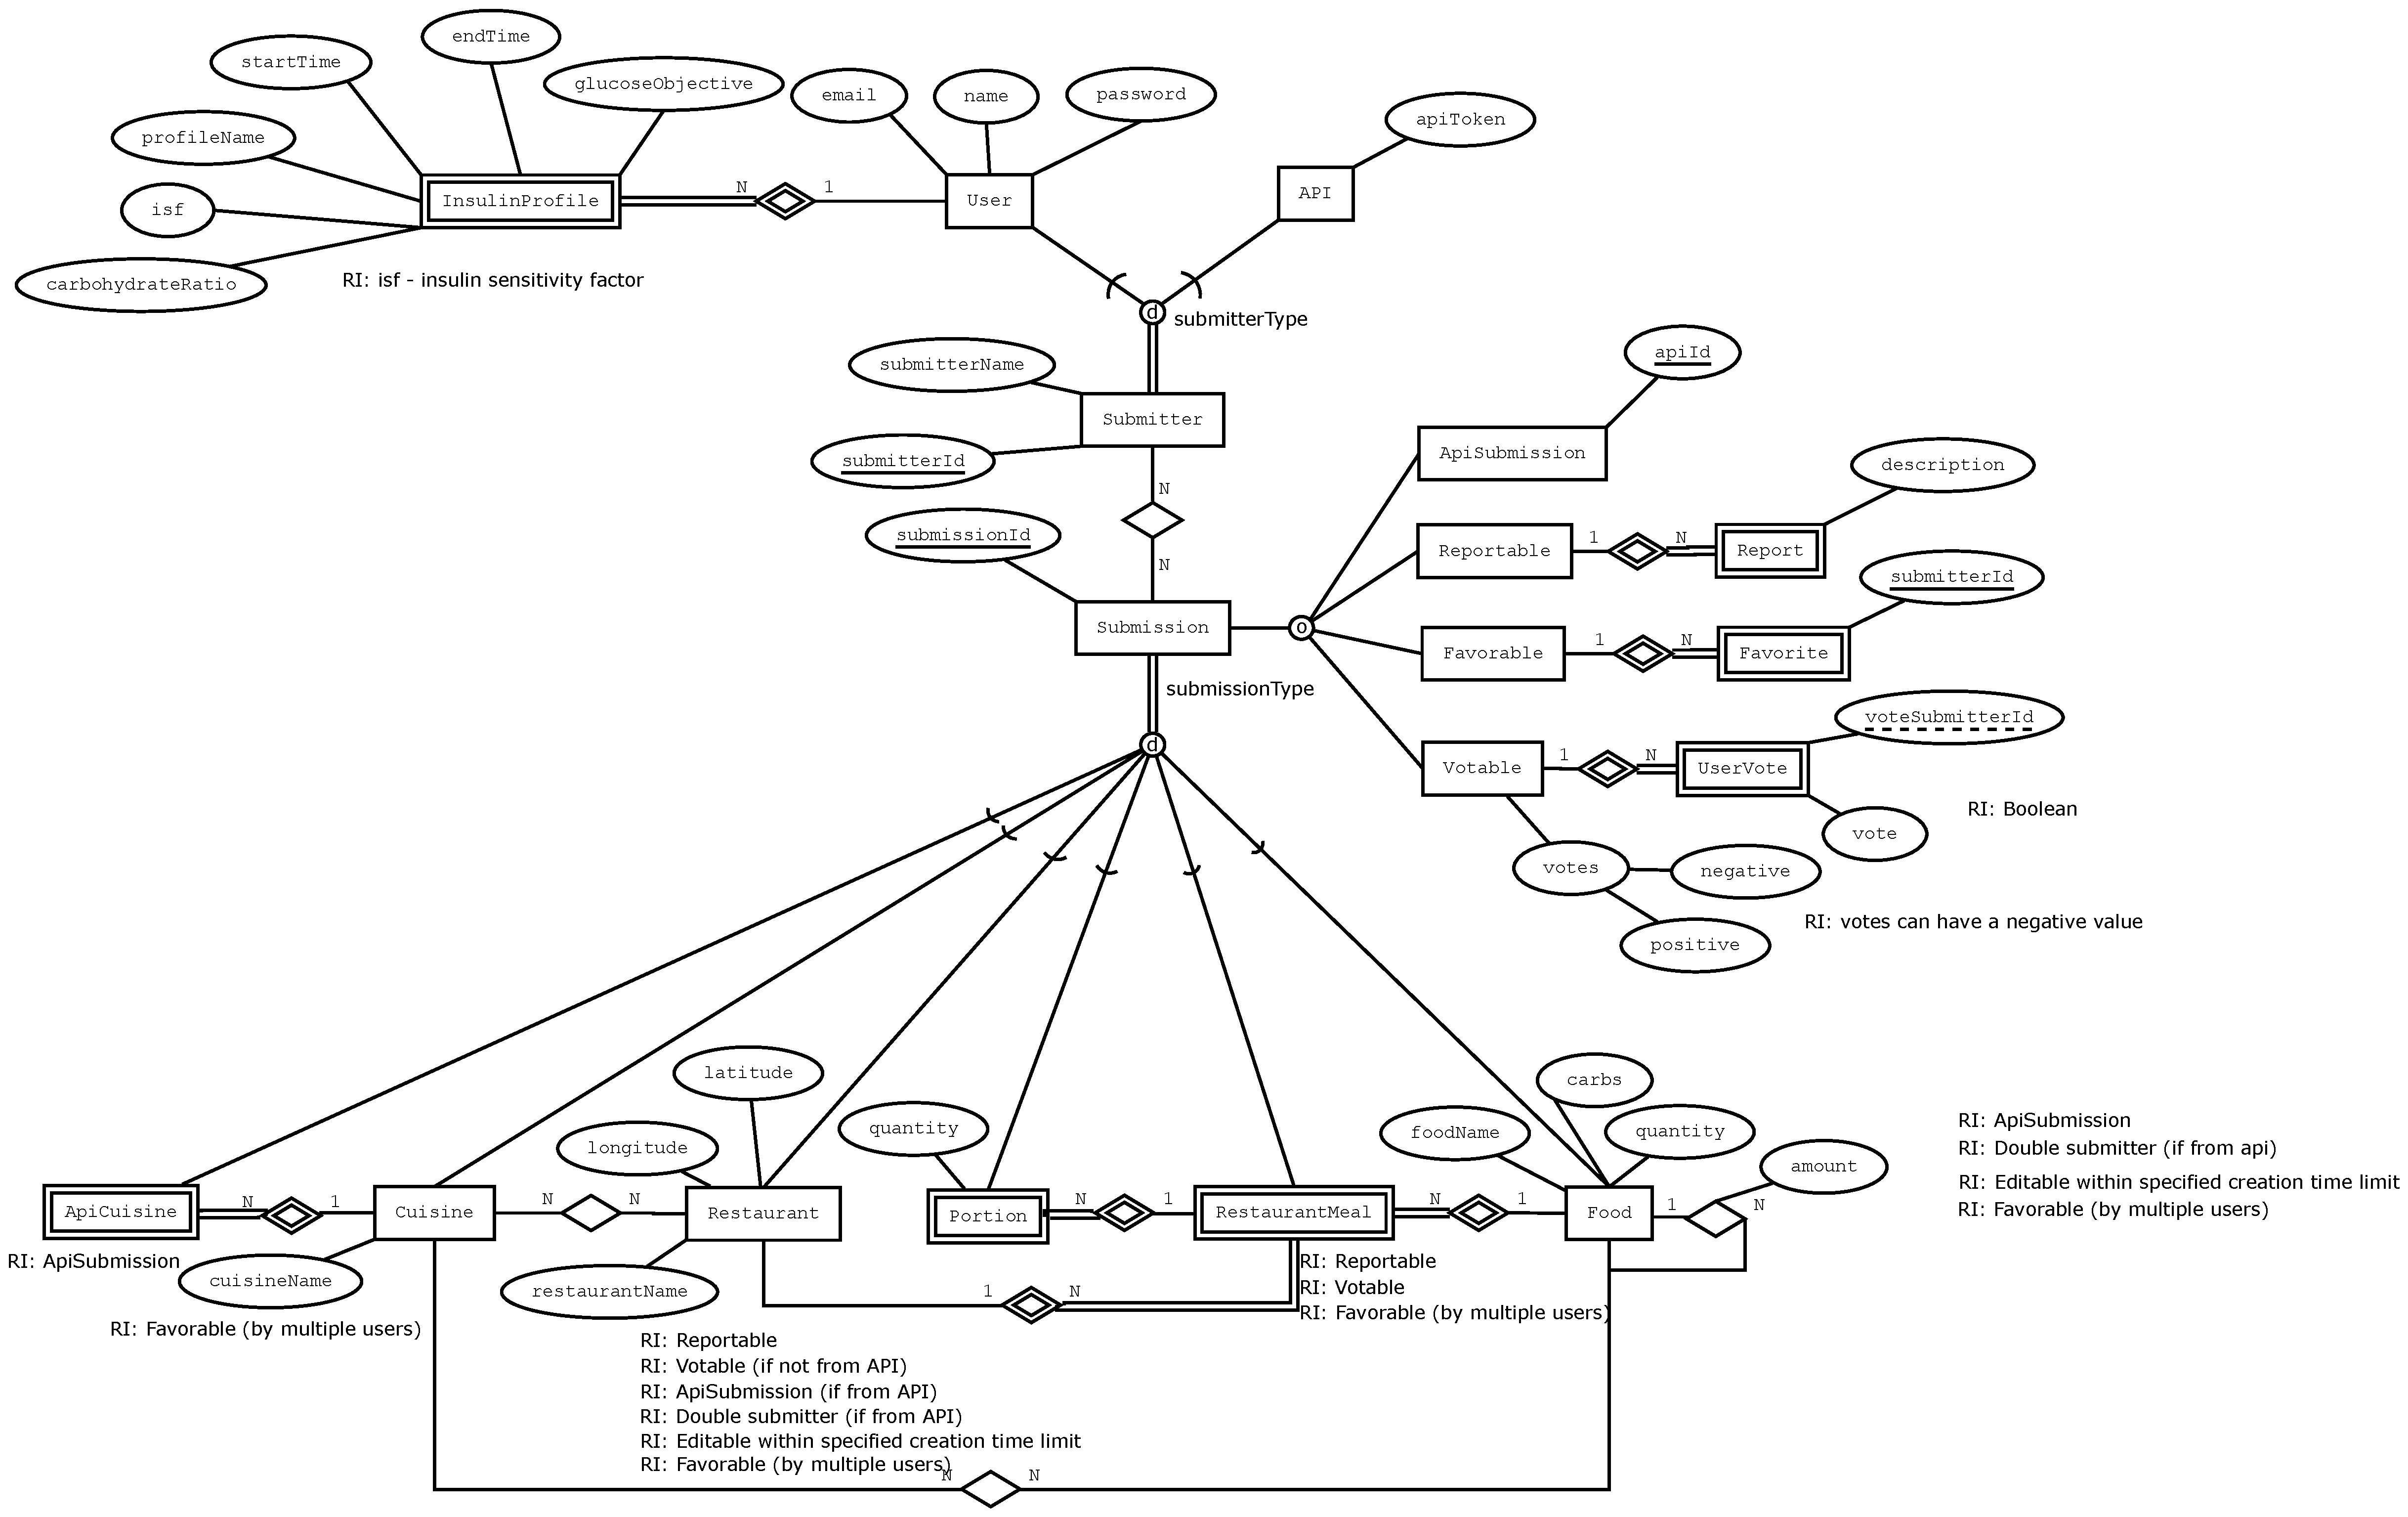
\includegraphics[scale=0.2]{_figures/Nutr.io_Database_Diagram.eps}
    \caption{Database conceptual model}
\end{figure}

The database's relational model is present inside this report's appendix [\nameref{app:relational_model}].\\

In the relational model there are tables which are not specified in the conceptual model.
These are a product from the normalization and associations between entities which will simplify queries' complexity.\\

A submission can fit into 4 categories: ApiSubmission, Reportable, Favorable and Votable, in order to disguish between submissions that
are from the user or from APIs and to separate which ones can be reportable, favorable and votable by the user.\\

The cuisine entity has an association called ApiCuisine in order to map cuisine identifiers unique to the Here API to our own cuisines.\\

A food is always one of the following: a suggested meal, a custom meal or an ingredient - all identified by their submission type (SM, CM and I, respectively).\\

A meal can also be composed by other meals or ingredients, represented by the 1-N Food association.\\

Regarding security and encryption, all sensible user information such as medical records in the InsulinProfile table 
or passwords in the User table are encrypted or hashed.\\

More details about security can be found in [Chapter 8 - Encryption and Sensitive data]\\

\section{HTTP server}

\subsection{Used tecnologies}

\subsubsection{Kotlin}

We chose to use Kotlin\cite{kotlin} for the HTTP server developed as it is a language that is being more adopted and used nowadays and because it is totally 
interoperable with Java\cite{java}.\\

It was also the language used during PDM, which is an optional course for Android application development inside the LEIC programme, 
making this a language we felt confortable with.\\

\subsubsection{Spring MVC}

At the beginning of the project we decided to use Spring MVC\cite{springmvc} rather than Ktor\cite{ktor}, as the first one is taught in DAW, which is an optional course
for Web applications development inside the LEIC programme. As Spring MVC has a better coverage inside the LEIC programme, we considered 
it a more solid choice.\\

\subsubsection{Used dependencies}

Here are all the dependencies injected inside HTTP server gradle settings file.\\

\begin{itemize}
    \item \textbf{Kotlin base dependencies} - kotlin-reflect and kotlin-stdlib-jdk8;
    \item \textbf{Spring base dependencies} - spring-boot-starter and starter-web;
    \item \textbf{Mockito} - for tests with mocks;
    \item \textbf{Jackson} - for JSON serialization and deserialization;
    \item \textbf{JDBI} - the driver/interface for connecting with the relational database;
    \item \textbf{Spring Security} - for authentication and authorization proposes.
\end{itemize}

\subsection{Code structure}

The HTTP server uses a Spring MVC implementation, structuring its' code in several layers:\\

\begin{itemize}
    \item MVC Controller layer, uses multiple services and handles input to model and model to
     output \textit{DTO} mappings through \textit{DTO} class mappers. Data Transfer Objects (\textit{DTO}):
     For every model there is an equivalent input and output \textit{DTO} class which is represented by its
     corresponding suffix, e.g. "\textit{InsulinProfilesInput}" and "\textit{InsulinProfilesOutput}".
     Controller classes are prefixed by "\textit{Controller}".
     \item Service layer, uses multiple repositories and handles model to database \textit{DTO} and database \textit{DTO}
      to model mapping through instance mappers. The mapper classes used to map the \textit{DTOs} to model have a domain prefix e.g.
      "\textit{Db}" or "\textit{Api}" while having a type "\textit{Mapper}" suffix e.g. "\textit{DbRestaurantMapper}". 
      The service class names are prefixed by "\textit{Service}". 
      \item Data Access layer, is ranged between repositories and Data Access Objects (\textit{DAOs}), each repository
       uses various \textit{DAOs} that represent each database entity/relation through JDBI declarative API. 
       For database \textit{DTOs}, the prefix "\textit{Db}" is used before the table name and then the suffix "\textit{DTO}". For \textit{DAOs} it was used the
       table name and the prefix "\textit{Dao}" e.g. "\textit{UserDao}". Repository classes are
       prefixed by "\textit{Repository}" e.g. "\textit{RestaurantDbRepository}". 
\end{itemize}

\begin{figure}[H]
    \begin{center}
        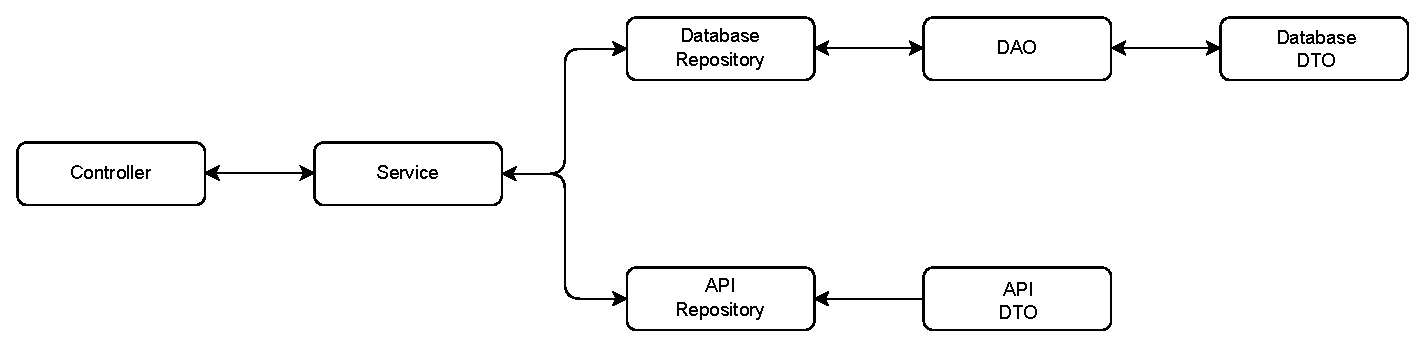
\includegraphics[scale=0.7]{_figures/server-classes.eps}
        \caption{Server's classes structure}
    \end{center}
\end{figure}

\subsection{Routing and endpoints}

\begin{figure}[H]
    \begin{center}
        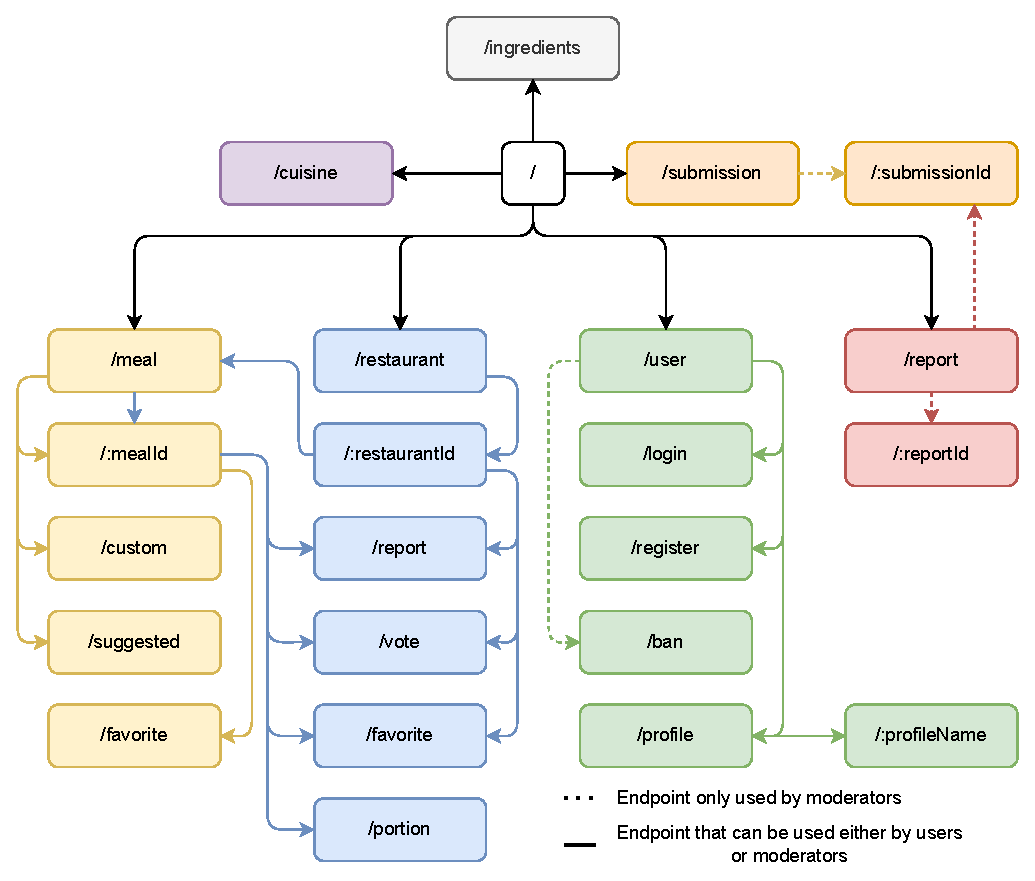
\includegraphics[scale=0.8]{_figures/endpoints_diagram.eps}
        \caption{The server's routing}
    \end{center}
\end{figure}

The picture presented above represents a simplified diagram that shows how the navigation between endpoints occurs.
It should be taken in consideration that, as the picture's label says, some nodes represented in this diagram are used by 
both users and moderators and the diagram can not label those situations with detail. Those details can be better analysed
in this report appendix about endpoints.\ref{app:endpoints_table} \\

The color code used in this diagram represents where each endpoint starts providing a better comprehension
and visualization, e.g.: /restaurant/:restaurantId/meal/:mealId (endpoint for a specific restaurant meal) starts with a blue
node (/restaurant); /meal/suggested (endpoint for suggested meals) starts with a yellow node (/meal).\\

\subsection{JDBI}

We decided to use JDBI as the library responsible for allowing communication between the server and the database due to teacher's
recommendations, integration with Spring and Kotlin, and finally its' declarative functionalities, which are explained further on.\\

As a brief description, JDBI is, according to the documentation:\\

"Jdbi is built on top of JDBC. If your database has a JDBC driver, you can use Jdbi with it.
Jdbi improves JDBC’s rough interface, providing a more natural Java database interface that is easy to bind to your domain data types.
Unlike an ORM, we do not aim to provide a complete object relational mapping framework - instead of that hidden complexity, we provide
building blocks that allow you to construct the mapping between relations and objects as appropriate for your application."\\

Although the documentation provided by JDBI describes in great detail its' functionalities and how to utilize them,
some key aspects and differences which are specific to the project are explained in the following sections.\\

\subsubsection{Getting started}

The \texttt{Jdbi} class is the main entry point into the library and each instance requires a \texttt{DataSource} connection,
which is created in the \texttt{DatabaseConfig} class according to the application properties provided in the resources folder.
A single instance of \texttt{Jdbi}, which in turn is used to create a single instance of \texttt{DatabaseContext}, the dependency that all
repositories require in order to perform database connections. 

\subsubsection{Database connection}

An active database connection is represented by a \texttt{Handle}, and according to the JDBI documentation:\\

A handle is used to prepare and run SQL statements against the database, and manage database transactions.
It provides access to fluent statement APIs that can bind arguments, execute the statement, and then map any results into Java objects.\\

Every database operation opens a new handle and is wrapped in a transactional call using \texttt{databaseContext.inTransaction(Function<Handle, T>)}.
Said transaction is committed when given function is successfully finished, or rollbacked if an exception is thrown. Finally, underlying handle
is only closed after the HTTP request that triggered the repository call is finished. This is due to Stream integration when returning database
elements and is explained in greater detail in next subsection: 5.2.5 - Fetching collections of data.

\subsubsection{Performance operations - Imperative and Declarative API}

When a repository uses previously mentioned method\\
\texttt{databaseContext.inTransaction(Function<Handle, T>)}, given argument function is responsible
for performing a database operation with the open handle, either using an \textbf{imperative} implementation or a \textbf{declarative} one.\\

The JDBI documentation describes both the imperative and declarative style as follows, respectively:\\

"The Core API provides a fluent, imperative interface, which uses Builder style objects to wire up your SQL to rich Java data types."\\

"The SQL Object extension sits atop Core, and provides a declarative interface. Tell Jdbi what SQL to execute and the shape of the results
you like by declaring an annotated Java \textit{interface}, and it will provide the implementation."\\

Additionally, the JDBI documentation offers a simple query example using both styles:\\

\begin{figure}[H]
    \begin{center}
        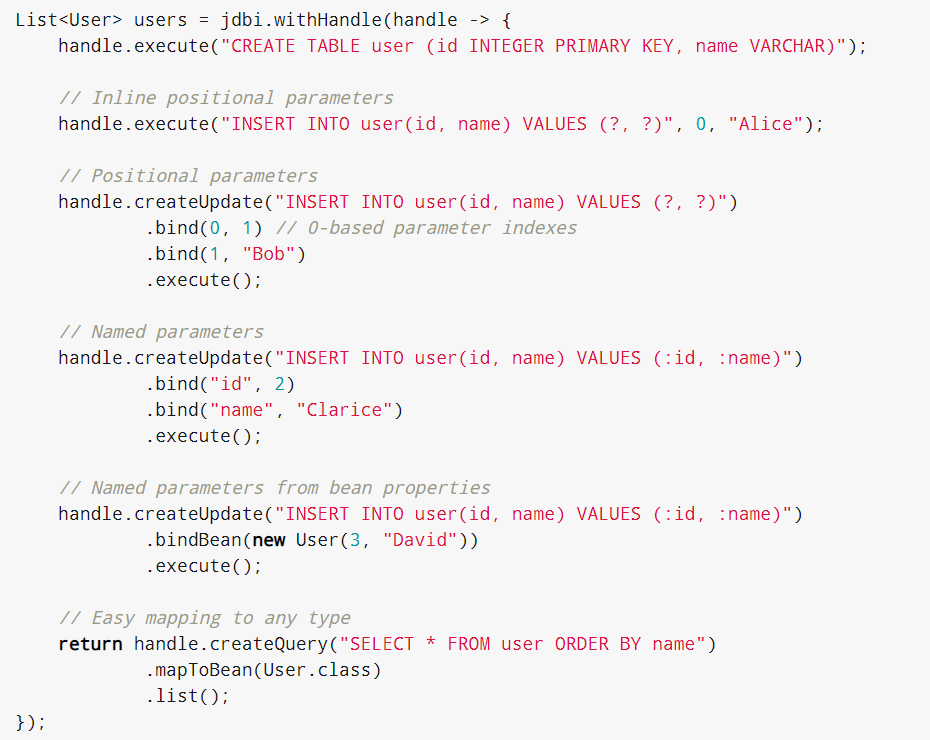
\includegraphics[scale=0.5]{_figures/imperative.png}
        \caption{JDBI imperative style}
    \end{center}
\end{figure}

\begin{figure}[H]
    \begin{center}
        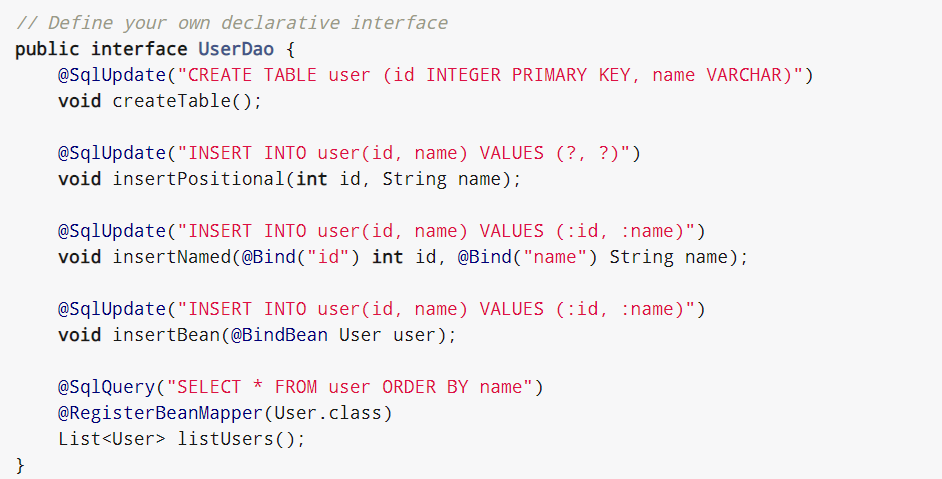
\includegraphics[scale=0.5]{_figures/declarative.png}
        \caption{JDBI declarative style - defining Data Access Objects}
    \end{center}
\end{figure}

\begin{figure}[H]
    \begin{center}
        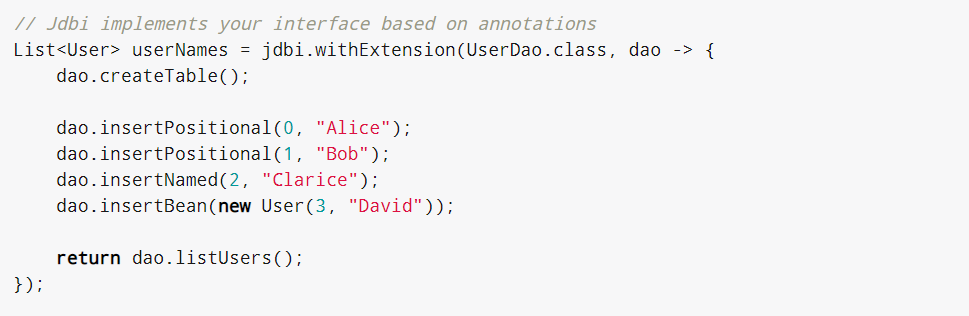
\includegraphics[scale=0.5]{_figures/calling-declarative.png}
        \caption{JDBI declarative style - Calling defined Data Access Objects}
    \end{center}
\end{figure}

In the context of our project, we use the declarative API due to its convenience and code simplicity over the
imperative one. The following is an example of a typical database operation in our application:\

\begin{figure}[H]
    \begin{center}
        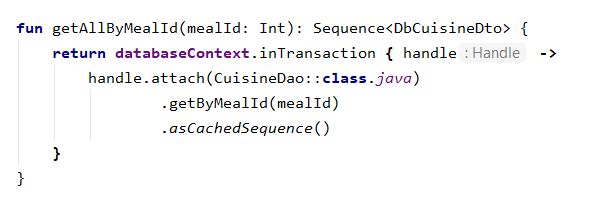
\includegraphics[scale=0.8]{_figures/jdbi-nutrio.png}
        \caption{Example of a database operation usin jdbi declarative type in our application}
    \end{center}
\end{figure}

\subsubsection{Avoiding multiple connections}

Throughout a single HTTP request lifetime, multiple database accesses can be performed. This is done in order to avoid querying
large quantities of data and then not needing it, and to support lazily acquired fields when building a model class.\\

However, if we consider that the information for each field is obtained in its' own and new transactional context then this
implementation can be performance heavy if we open multiple database connections as needed.\\

In order to avoid this, each HTTP request holds a single database connection if needed and closes it when completed, as we
can assume that no more database data is needed afterwards. This implementation is done by having every repository depend on
a single instance of the \texttt{DatabaseContext} class which opens a connection handle when needed and stores it in a 
\texttt{ThreadLocal} map, allowing for later removal by the \texttt{DatabaseCleanupInterceptor} interceptor.\\

Given implementation avoids mentioned issues, however it also introduces new issues that need to be taken into consideration,
such as only closing transactions when the interceptor is called - meaning that lengthy controller operations may lock database
tuples for longer periods of time, depending on the used transactional isolation level;  or the fact that a handle is linked to
a Thread identifier when created and deleted, so repositories calls must not be done under a different Thread than the interceptor one.\\

\subsection{Fetching collections of data}

When it comes to fetching collections of data (such as restaurants, meals, etc.) from either the database or an API, said data can be obtained
and iterated in an \textbf{eager} approach or a \textbf{lazy} approach.\\

We decided to implement the fetching of data in a \textbf{lazy} manner using Kotlin's \textbf{Sequences}\cite{sequences} instead of Java 8
\textbf{Streams}\cite{streams} due to their additional iterating operations, easier caching mechanisms (when compared to Streams)
and finally improved performance when processing data, according to the documentation:\\

"Sequences let you avoid building results of intermediate steps, therefore improving the performance of the whole collection processing chain."\\

Finally, sequences were chosen over streams because they can be reused and are not \textit{onceOf}(can only be used once) like streams.\\

With that in consideration, the following sections describe in greater detail the code structure needed to lazily acquire data.\\

\subsubsection{Database fetching}

According to the JDBI documentation\cite{jdbi}, a query method supports the return of lazy
collections using \textbf{Streams}, \textbf{ResultIterables} and \textbf{ResultIterators}:\\

"Query methods may also return a ResultIterable\cite{resultiterable}, ResultIterator\cite{resultiterator}, or a Stream\cite{streams}."\\

"As long as your database supports streaming results (for example, PostgreSQL will do it as long as you are in a transaction and set a fetch size), the
stream will lazily fetch rows from the database as necessary."\\

Since no native support for Sequences exist, every DAO class returns a ResultIterable of data and calling repository is then responsible of mapping it to
a Sequence via\\
\texttt{IterableUtils.asCachedSequence()}, an created extension method which also caches acquired values allowing for subsequent iterations.\\

However, this approach is not enough on its' own as JDBI warns that:\\

\texttt{ResultIterable}, \texttt{ResultIterator} and \texttt{Stream} methods do not play nice with on-demand SQL Objects. Unless the methods are called in a nested way, the
returned object will already be closed.\\

Given the following, it is simply not enough to have every \textit{DAO} and Repository class return a lazy collection after a handle/transaction call,
as the returned collection would be closed; so a solution was needed.\\

An initial solution involved opening a connection handle to fetch a Sequence of data and closing said handle when a terminal operation is executed, meaning that all data was
safely extracted and cached. This solution proved to not be programmer friendly and with dangerous pitfalls, and as such was discarded since nothing "forced" the programmer to
perform a terminal operation which would lead to resource leakage.\\ 

Another alternative is to wrap a repository call in a nested way, as the JDBI documentation suggests. This approach relies on leaking database logic and dependencies to Controller
and/or Service classes, which goes against a clean dependency injection design and as such was also discarded.\\

Finally, the adopted solution ties perfectly with the issues and developed solutions mentioned previously in chapter \textbf{5.2.4 JDBI} regarding \textbf{"Avoiding multiple connections"}.
If we assume that a Sequence and its' resources are no longer needed after the underlying HTTP request is closed, then having the \texttt{DatabaseCleanupInterceptor} class close the
database connection avoids resource leakage when given sequences are not operated in a terminal way and having Controller and Service classes rely on database  related logic.


\subsection{Request lifecycle}
Each request is received in a spring controller mapping, with input object,
parameters or path variables as arguments. When receiving an input object \textit{DTO},
it will be validated with java's \textit{javax.validation} (Hibernate).
Once validated the input model's data might be used in subsequent service layer calls.\\

Repositories are used on the service level to handle all \textit{DAO} interactions with
the database and other HTTP API requests. The resulting responses (input and database \textit{DTOs})
are converted to the model \textit{DTOs} according to their response mappers.
All API calls are made from asynchronous HTTP requests, while database calls block the calling thread.\\

\subsection{Restaurants}

Unlike other submissions, restaurants can be obtained from two sources of truth - APIs and the database -
creating obstacles that needed to be solved and explained in this section, such as data consistency and defining unique identifiers.\\

\subsubsection{Data consistency}

Restaurants provided by APIs are only copied to the database when new metadata is added (such as a user vote, meal or favorite) in order
to avoid creation of unnecessary and duplicate tuples. After a restaurant is copied to the database with new metadata, the server ensures
that subsequent requests always return the database submission and not the API one by prioritizing database results.\\

When searching nearby restaurants by location, this is done by querying both the database and the API and removing API results if their
identifier already exists in the database result. When requesting a specific restaurant, the server prioritizes searching the database
first and only the API afterwards, if no initial result was found.\\

\subsubsection{Unique identifiers}

Given that restaurants can be obtained from two sources of truth, then we can consider that each source provides its' own unique identifier.
A mechanism that merges identifiers needed to be implemented in order to avoid not knowing which source contains requested restaurant with
identifier \textbf{"ID1"} or worse - having two different restaurants from different sources with the same identifier.\\

Said mechanism is \textit{RestaurantIdentifier}, which always contains the submitter in order for the server to know from which source the restaurant
is from, and may contain a database submission identifier and/or an API identifier. Additionally, when an API restaurant is copied to the database,
its' \textit{RestaurantIdentifier} will now contain both API and database identifier.\\

When a request is done with an outdated \textit{RestaurantIdentifier} (one that represents a restaurant which is contained in the database but has no respective
identifier), the server always queries the database first under the submitter and API submission pair in order to ensure data consistency. This behavior
can be observed in the \textit{RestaurantServiceTests} class.

\subsection{Pagination}

Some endpoints return lists to the clients, and as such these endpoints should not return all the items available that are associated
to them in order to avoid the server from fetching big quantities of data, high transfer times of said data to the client and 
high memory usage on the client side.\\

To solve this issue we decided to implement a basic pagination mechanism, by implementing features in the following layers:\\

\subsubsection{Controller}

For endpoints that have pagination, two optional query parameters were added: skip and count. These two, for most cases, have a
default value which is used when the client does not specify these parameters and, when they do, said values are also validated 
according to the following constraints:
\begin{itemize}
    \item Skip and count must not be negative;
    \item Count must not be higher than the server maximum defined value: currently 40 items.
\end{itemize}

\subsubsection{DAO}

Database pagination is achieved using PostgreSQL LIMIT and OFFSET keywords.\\

The first one specifies how many items a result should hold and its' value is equal to count,
while the second one represents how many objects should be skipped and as such, its' value is count
parameter multipled by the skip parameter.\\

\subsection{Spring Security}

\subsubsection{JSON Web Tokens}

As each client needs to have authentication to provide the user a way to create an account and allow submissions and data synchronization,
we had to discuss about the platform's security and the safest ways to do that.\\

It was concluded that the use of \textbf{JSON Web Tokens}\cite{jwt} was the best option, because of the nature of the clients, more specifically the fact that
the mobile application is completely \textbf{stateless}.\\

Another advantage is the fact that these tokens have an expiration time, which means that after a certain amount of time they are no longer valid.
In case of security breach, this feature becomes useful, because if a valid token is stolen, neither the attacker has a way to generate valid tokens 
nor does he know the user's password. The token could only be used by a short period of time (10h), easing the amount of damage that an intruder can
make and confining it to only one user inside the platform.\\

The picture below represents a very generic and simplified workflow of the JSON Web Token. 

\begin{figure}[H]
    \begin{center}
        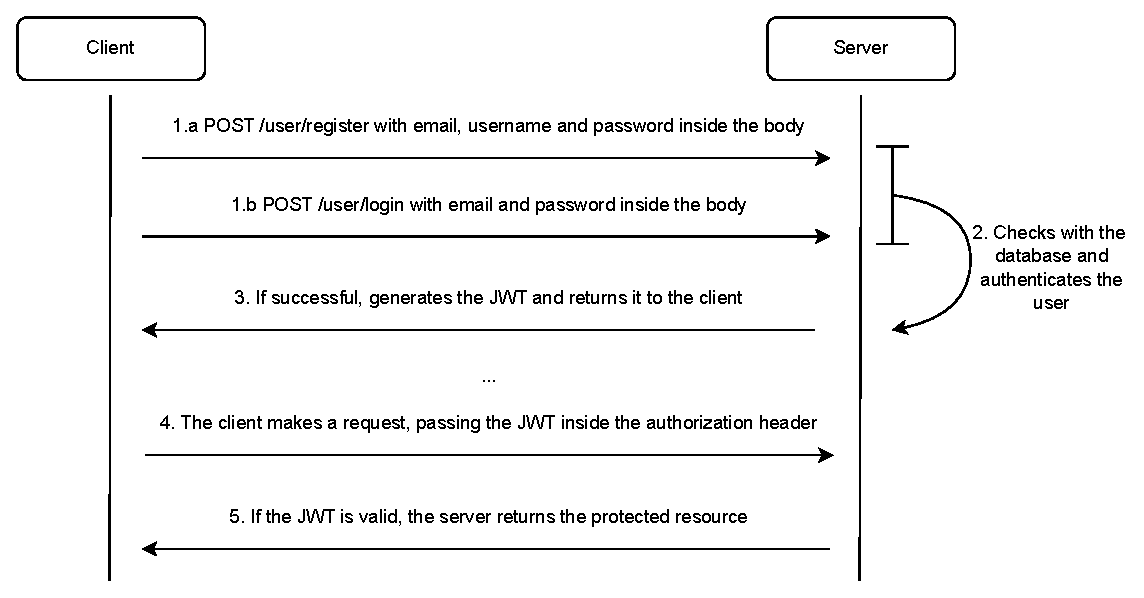
\includegraphics[scale=0.9]{_figures/JWT-simple-diagram.eps}
        \caption{The JWT workflow}
    \end{center}
\end{figure}

\subsubsection{Implementation}

To implement the shown workflow inside the HTTP server, as we are implementing it with Spring, the more obvious choice was to use \textbf{Spring Security}\cite{springsecurity}.\\

Spring Security is a customizable authentication and access-control framework.\\

The picture below shows how the server handles an user login using this framework.\\

\begin{figure}[H]
    \begin{center}
        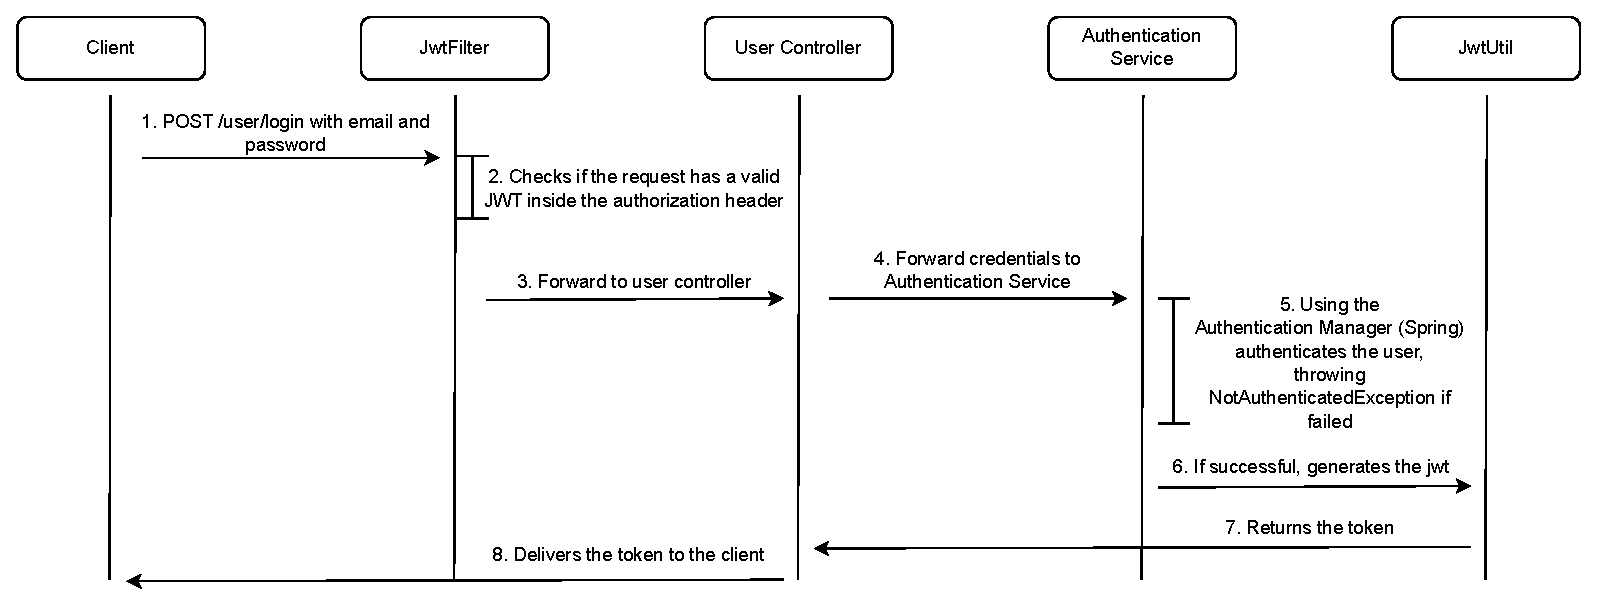
\includegraphics[scale=0.60]{_figures/Spring-jwt-diagram.eps}
        \caption{A Spring security workflow example with the POST /user/login}
    \end{center}
\end{figure}

After the previously mentioned dependencies are installed, the WebSecurityConfig is the first class to be constructed. Here are specified, via antMatchers, which
endpoints do not need authentication, acting like a whitelist, so every endpoint that is not specified via antMatchers needs authentication, and will return code 401
Unauthorized if the JWT is invalid. The JWT filter is also started up inside this class.\\

The UserAuthenticationArgumentResolver class, as the name says, is an argument resolver that filters each request, acting before it reaches the desired controller,
checking the authentication header and extracting the jwt from the Bearer verifying if it is valid.\\

The Authentication service class calls the Spring Authentication Manager and authenticates the user, it provides methods which call the JwtUtil
to retrieve the email from the token or encode the password when registering.\\

The password encoding always happens when the user registers for the first time: the server hashes the password using \textbf{BCrypt}\cite{bcrypt} before inserting the new
user into the database.\\

BCrypt is a password-hashing function based on the Blowfish\cite{blowfish} cipher. We found this function very convenient for these reasons:
\begin{itemize}
    \item Already pre salts the passwords, preventing rainbow table attacks\cite{rainbowtable};
    \item Makes bruteforce attacks inviable: the iteration count can be increased to make it even slower to crack.
    This cipher makes even GPU-powered bruteforce attacks impracticable due to this feature.
\end{itemize}

The JwtUtil is the core class which validates, generates and adds claims to the tokens.\\

\subsection{User data safety}

In the previous section it was shown that the user can register an account. It was made this way so the server can store
insulin profiles, which will be better explained in the mobile application's section. The insulin profiles store user sensitive
information and are encrypted when written inside the database using a symmetric cipher (AES-256) with a private key provided by an 
environment variable from the host machine.\\

The user can also delete its account. When an account is deleted all user sensitive information is deleted from the server: email,
username, password, insulin profile and custom meals. However, its submitter identifier, which is a database generated number,
is maintained in order to preserve its public submissions, in order to keep the platform's data consistent, so a user that makes many 
public insertions does not compromise our data's consistency if its account is deleted.\\

This way we also comply to the General Data Protection Regulation (GDRP)\cite{gdpr}, as we are keeping data safe by encrypting it into the database and
we are not collecting user's data for other interests and, the most import of all, we provide the user the right to be erased from our 
platform removing every personal detail from it when an account deletion happens.\\

\section{Geolocation}

Given how all clients rely on obtaining nearby restaurants, there was a need to implement a geolocation function in the project's design.\\

Initial research showcased two possible solutions: Haversine\cite{haversine} distances and cartesian distances, where the latter returns a highly imprecise distances.
As such, Haversine was selected.\\

The next step was to choose which system filters nearby restaurants: database or HTTP server. After some discussion, we decided that database was the best
option for two reasons: 
\begin{itemize}
    \item Given the large amount of existing restaurants, sending such data from the database to the HTTP server so that it could filter it would occupy too much memory;
    \item PostgreSQL already supplies extensions that add support for location queries, namely PostGIS.
\end{itemize}

\section{Android application}

\subsection{Used tecnologies}

\subsubsection{Kotlin}

We chose to use Kotlin for the mobile application development, as it is now the official programming language for Android development,
according to Google.\\

It is also the language taught during the optinal course - mobile devices programming (PDM).\\

\subsubsection{External dependencies}

Here are the dependencies that were included in the mobile application which gave more functionalities to it.

\begin{itemize}
    \item \textbf{Volley} - an HTTP library for Android networking;
    \item \textbf{Jackson} - JSON serialization, deserialization and handling;
    \item \textbf{Room} - A framework to store data locally;
    \item \textbf{MapBox} - A framework to provide maps and geolocation tools;
    \item \textbf{MPAndroidChart} - provides custom graphs inside the application;
    \item \textbf{Glide} - a framework for image loading;
    \item \textbf{FlexBox} - a library which adds the flexible box layout, in order to hold multiple items
    inside the same box;
    \item \textbf{Androidx crypto} - a new crypto library made by Google, used to encrypt User credentials.
\end{itemize}

\subsection{Code structure}

\subsubsection{Drawing pattern}

The mobile application code structure follows the \textbf{repository pattern}, which is a code architecture recommended by the \textbf{Android Jetpack}\cite{jetpack} for this type of applications.\\

\begin{figure}[H]
    \begin{center}
        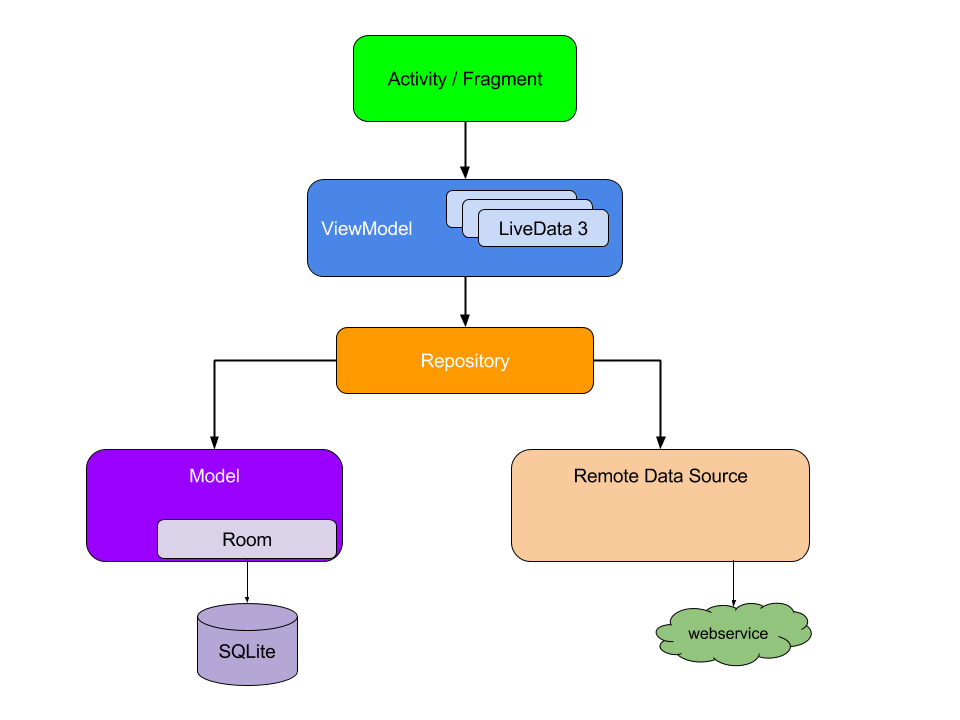
\includegraphics[scale=0.5]{_figures/repository_pattern2.png}
        \caption{The repository pattern diagram}
    \end{center}
\end{figure}

Above there is the pattern's diagram provided by the Android Jetpack.\\

The idea behind this architecture is that each Activity or fragment has its own ViewModel and each one calls the needed functions present inside the repository.
The repository is a layer that manages where the information should be retrieved from.\\

The 'DTO to model' mapping also occurs inside the repository, following the rule where ViewModels should only manipulate models and the layers below should only use DTOs.\\

By following this pattern, the code becomes segmented and organized, allowing a good comprehension and code maintainability.\\

Just as the server the android client has the input and output "\textit{DTOs}" suffixed with "\textit{input}" and "\textit{output}". 
These classes are mapped by input mappers prefixed with "\textit{input}".\\

The Activity, Fragments, ViewModel, Adapters and Repositories classes are all prefixed by their type.

\subsubsection{Fragments}

We chose to use fragments\cite{fragment} for each application view instead of activities. Although a fragment has a more complex lifecycle than the activity and depends on it
to exist, they are far more lightweight to instanciate than an activity and thus they provide more performance to the application.\\ 

It is also the recommended Android widget to use when designing an application with a side drawer.\\

\subsubsection{Modular interfaces}

As the code in the mobile application development became repetitive, the group decided to implement modular interfaces,
which are interfaces that can be implemented by fragments and viewholders and provide them predefined behaviours.

\subsection{Local data storing}

As mentioned in the dependencies, the mobile application utilizes Room to store data locally. This is convenient
for multiple reasons: 
\begin{itemize}
    \item To allow using the application in offline situations;
    \item To save data in order to avoid unnecessary requests to the server;
    \item To help data synchronization, that will be detailed later in this section.
\end{itemize}

Room classes use the "\textit{Db}" prefixed followed by the name and prefixed by their type e.g. "\textit{DbMealInfoMapper}", "\textit{DbMealInfoRelation}" and "\textit{DbMealInfoEntity}". 
The \textit{DAO} classes However are only prefixed with "\textit{Dao}". 
All entities are mapped by a database mapper suffixed with "\textit{Mapper}".

\subsection{User authentication and authorization}

The user has the ability to register and login in the mobile application. Besides being the server responsable for these functions, the mobile application has also some intervention
here, because after a successful login or register, the HTTP server will return a jwt (JSON Web Token) that will authenticate and authorize the user in future requests.\\

This token will be stored in the Android Shared Preferences\cite{sharedpreferences} and it will also to be renewed periodically due to its 10h expiration time. The user credentials will also be saved
inside the mobile device to allow automatic logins to renew the user's JSON Web Token and avoid its expiration.\\

\subsubsection{Problem: The content inside the shared preferences is written in plaintext. Is it safe to store user credentials inside the shared preferences?}

Although the Android Shared Preferences being a safe place to store application information, this fact is not completely true:
a normal device can not access these preferences and it should be a safe place to store user credentials, however rooted devices\cite{root} can easily
access the shared preferences file and retrieve plaintext from it, which would compromise the user security.\\

\subsubsection{Resolution: Androidx Crypto}

The Androidx crypto\cite{crypto} was used to solve this issue. This library is used to encrypt the user credentials before writing them inside the mobile device.\\

These new Google library takes advantage of the Android KeyStore\cite{keystore} system, which encrypts information using a hardware-level encryption, making the
encryption even harder to break. The information is encrypted using a symmetric cipher algorithm (AES-256), the key used to sign and encrypt information
is hardware-generated and it is managed by the application itself, so the key's retrieval from an 'encrypted' shared preferences is equal to the 'normal'
shared preferences.\\

We also discussed if the credentials should be saved inside the device or if only the database should possess them.
If that approach was taken, the user had to login each time it was needed to read or write a protected resource.\\

As this platform is not, for example, a bank application that needs top protection. We found this level of protection
unnecessary for the application and inconvenient for the user and decided that only the essential protection should be provided - 
user credentials encryption to avoid information leaks from rooted devices.

\subsection{Android version compatibility}

In order to garantee a global support by most of the Android devices nowadays, the mobile application is supported since \textbf{Android 7} (API level 24)
up to \textbf{Android 10} (API level 29).

\subsection{Functionalities}

Here will be displayed pictures of the mobile application and its functionalities.\\

\subsubsection{Register and Login}

\begin{figure}[H]
    \captionsetup[subfigure]{justification=centering}
    \begin{center}
        \begin{subfigure}{.3\textwidth}
            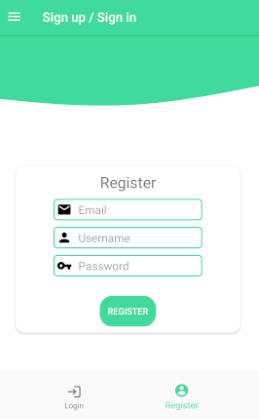
\includegraphics[scale=0.1, width=\textwidth]{_figures/register.png}
            \caption{The register fragment} 
        \end{subfigure}
        \begin{subfigure}{.3\textwidth}
            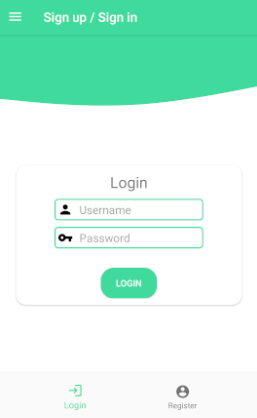
\includegraphics[scale=0.1, width=\textwidth]{_figures/login.png}
            \caption{The login fragment} 
        \end{subfigure}%
        \begin{subfigure}{.3\textwidth}
            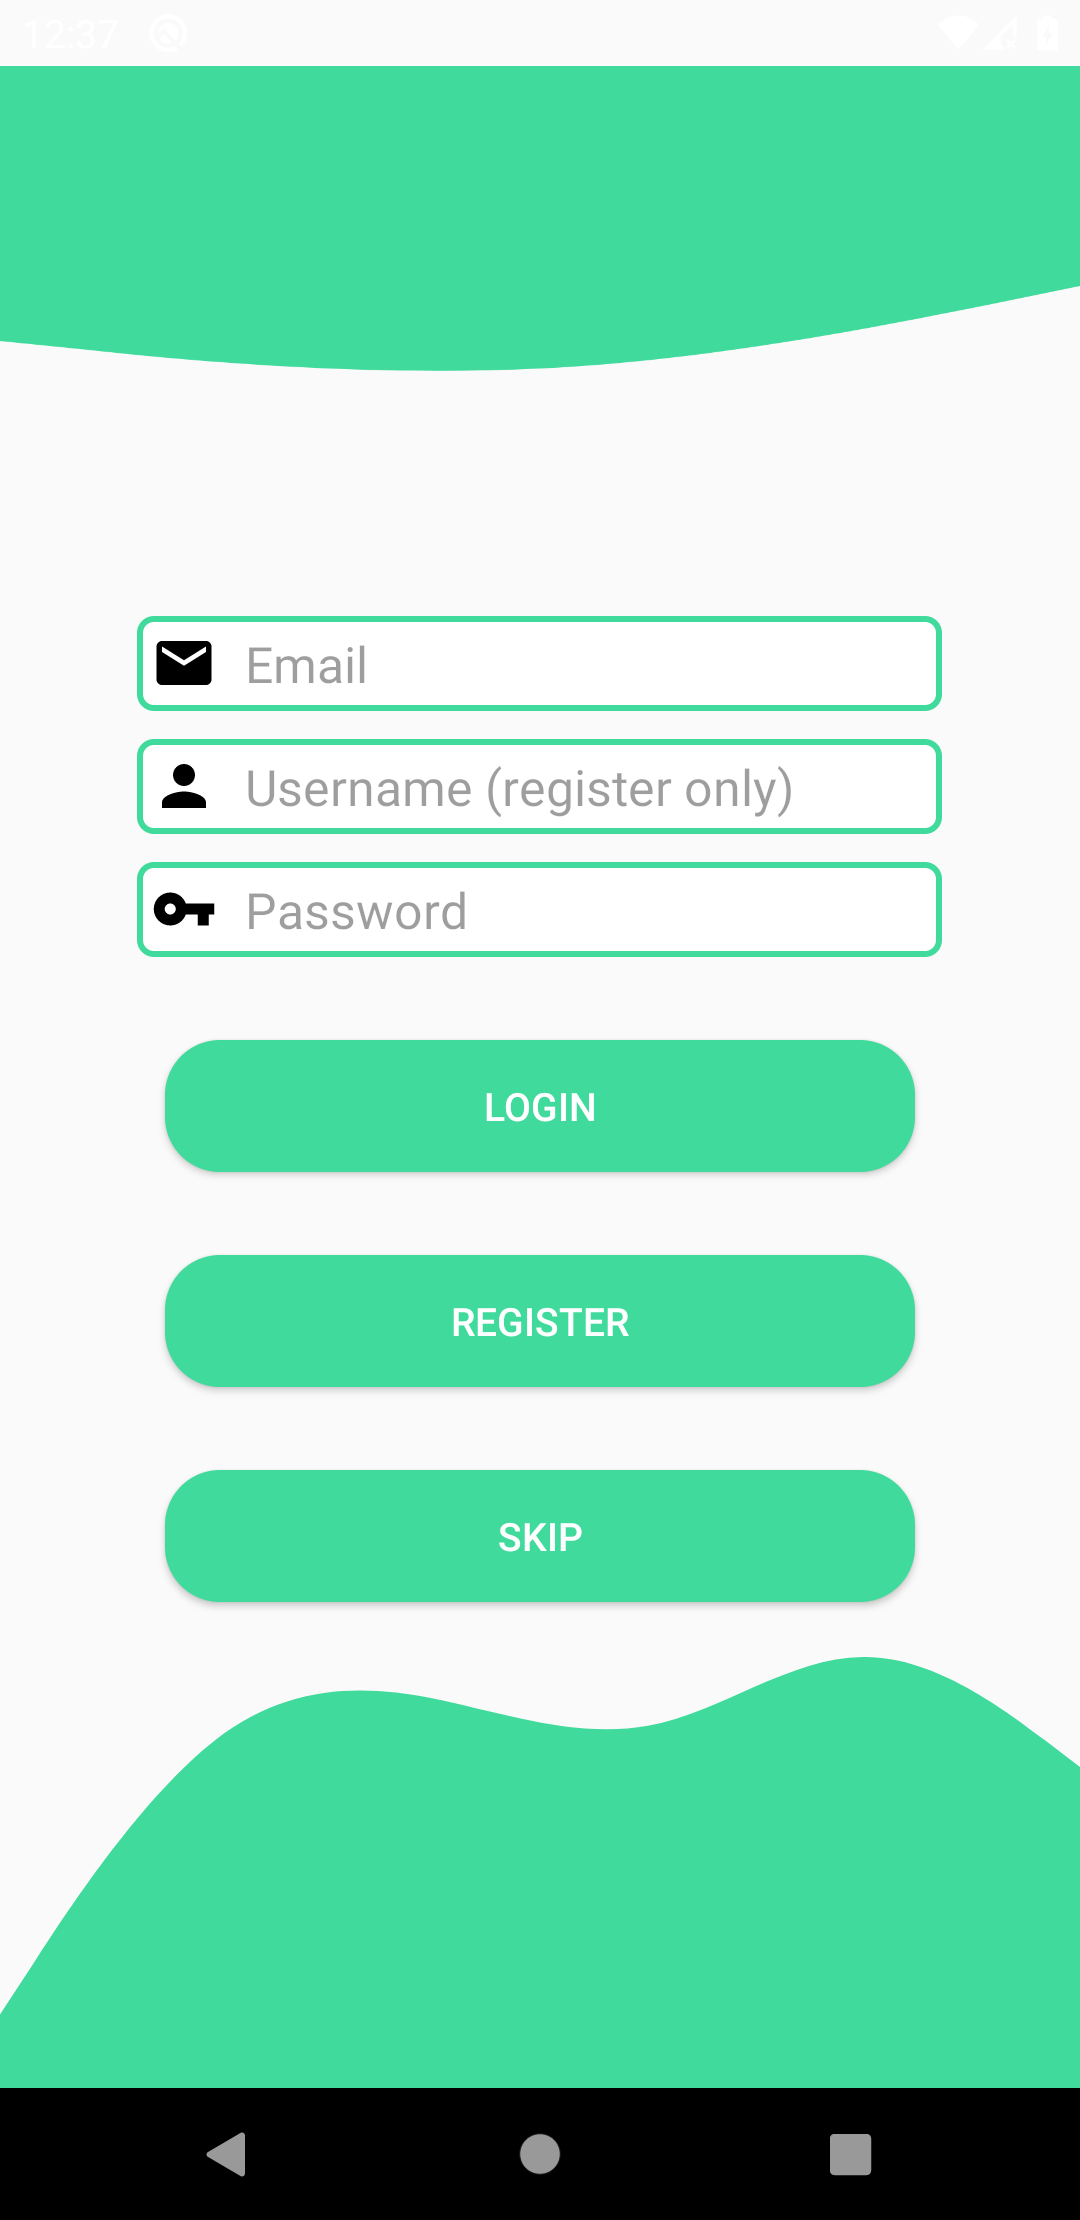
\includegraphics[scale=0.1, width=\textwidth]{_figures/firstSign.png}
            \caption{The sign in/up at the application's startup} 
        \end{subfigure}%
    \end{center}
\end{figure}

Here are the 3 ways a user can register or login inside the mobile application: either on the application's startup or by clicking on the user's profile picture inside the
drawer menu and accessing the slide screen with the bottom bar.\\

Here's the login and register workflow:

\begin{figure}[H]
    \begin{center}
        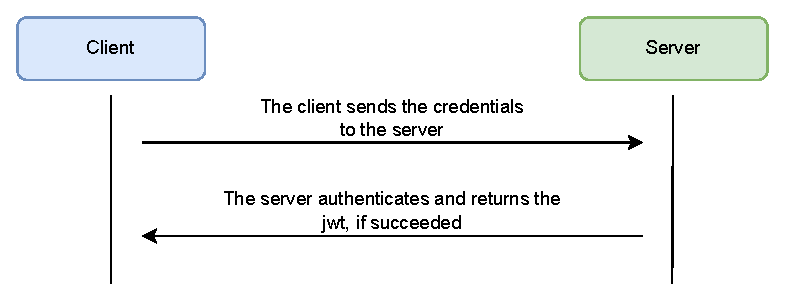
\includegraphics[scale=1]{_figures/auth-workflow.eps}
        \caption{Login and register workflow}
    \end{center}
\end{figure}

\subsubsection{Account deletion}

If the user goes to the login or register fragment again after being successfully logged in, it will see the fragment presented below.

\begin{figure}[H]
    \centering
    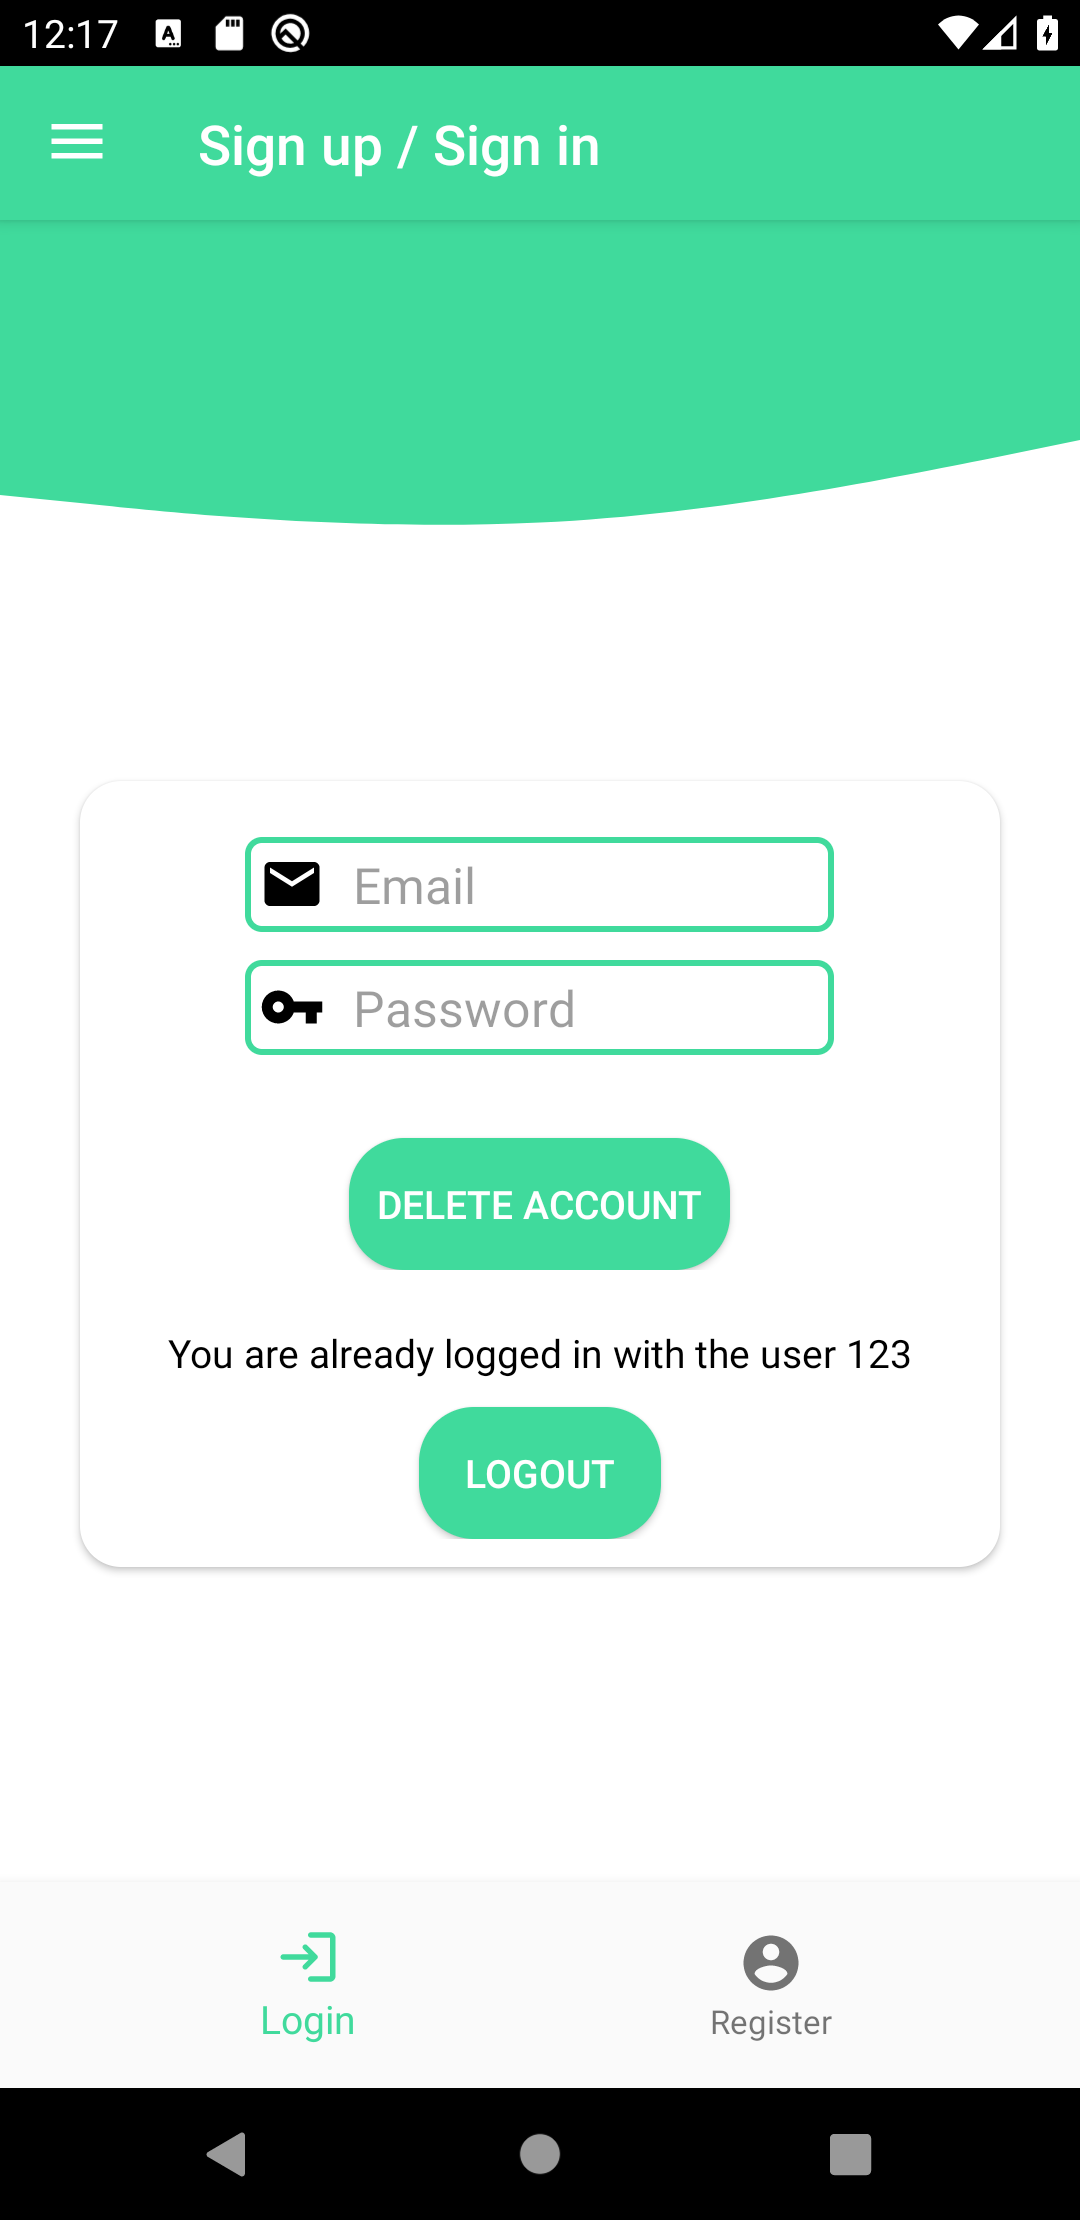
\includegraphics[scale=0.12]{_figures/logout_fragment.png}
    \caption{The register fragment}
\end{figure}

In order to delete the account, the user needs to fill the shown form again and then press the delete account button.\\

After that, the operation will occur as the diagram presented below.

\begin{figure}[H]
    \begin{center}
        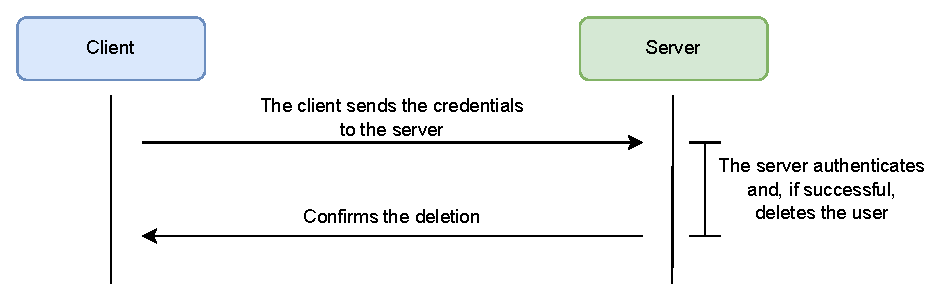
\includegraphics[scale=1]{_figures/user-deletion-workflow.eps}
        \caption{User account deletion workflow}
    \end{center}
\end{figure}

After this only the submitter identifier will remain in database to preserve public submission and all sensitive data
will be deleted.

\subsubsection{Insulin profiles' creation and access}

\begin{figure}[H]
    \captionsetup[subfigure]{justification=centering}
    \begin{center}
        \begin{subfigure}{.3\textwidth}
            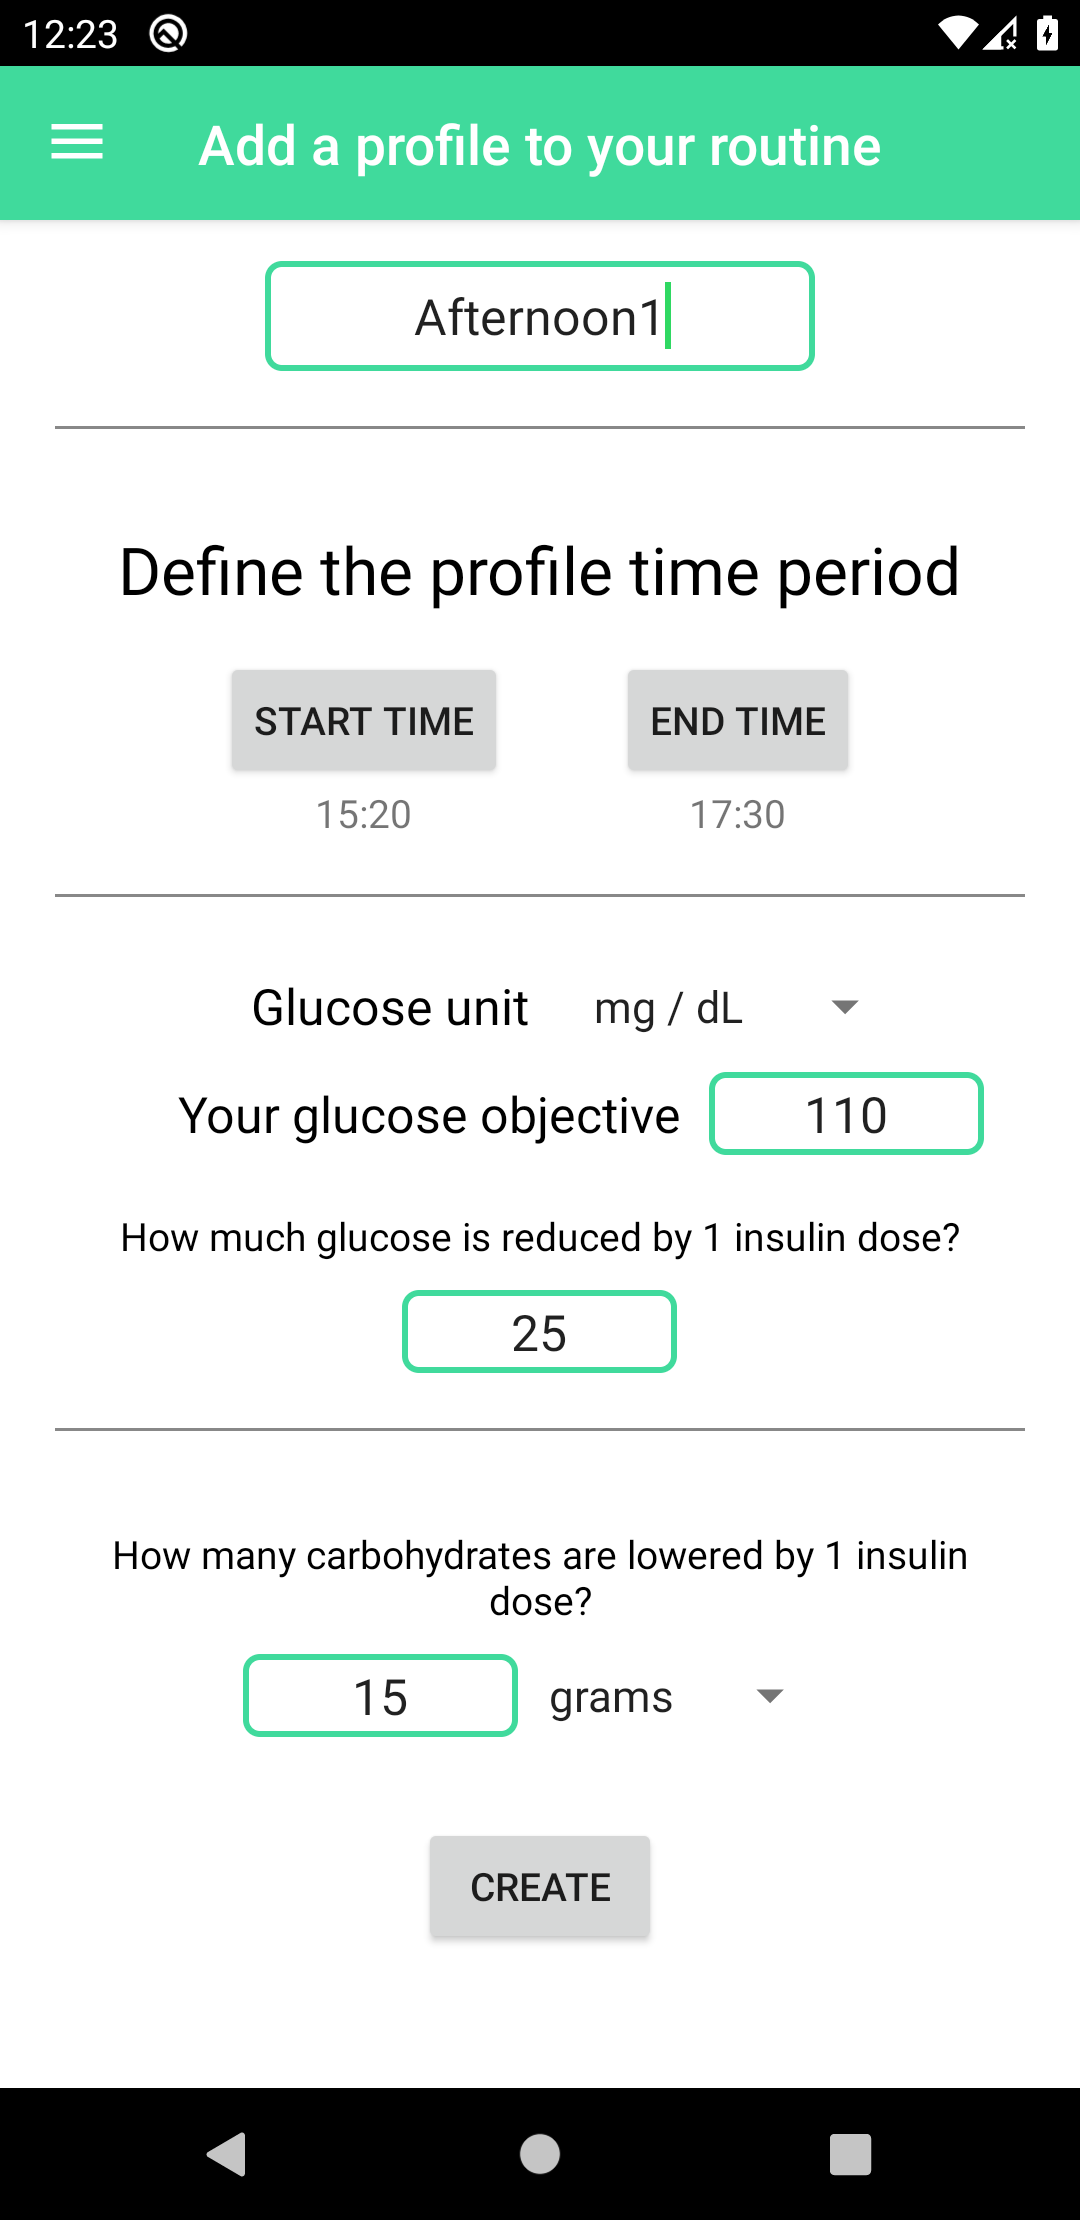
\includegraphics[scale=0.1, width=\textwidth]{_figures/addProfile.png}
            \caption{The fragment to add an insulin profile} 
        \end{subfigure}
        \begin{subfigure}{.3\textwidth}
            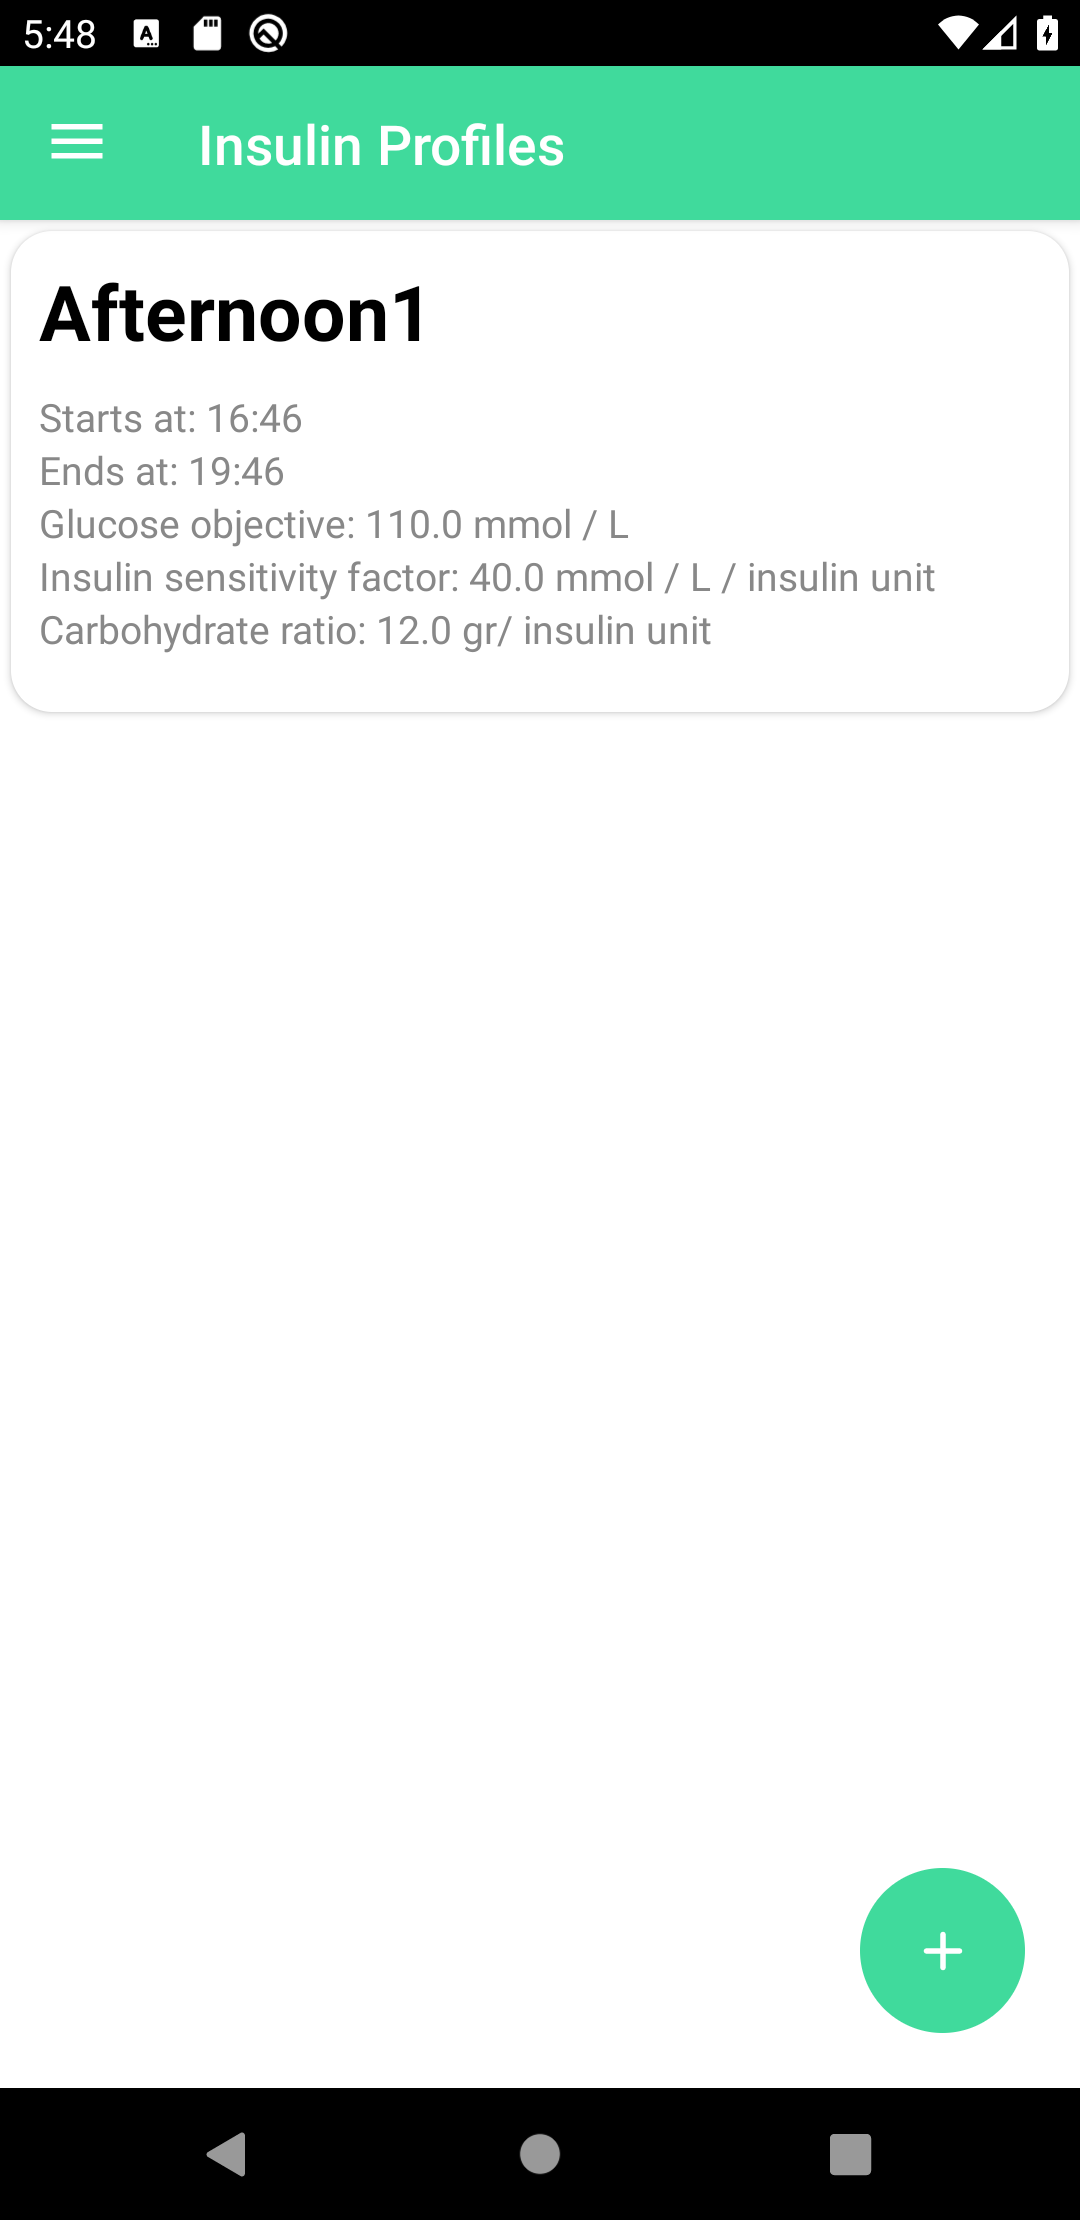
\includegraphics[scale=0.1, width=\textwidth]{_figures/insulin_profiles_list.png}
            \caption{The fragment to access and create insulin profiles} 
        \end{subfigure}
    \end{center}
\end{figure}

The user can map its day with insulin profiles, specifying for a certain timespan its glucose objective, insulin sensitivity and carbohydrates sensitivity, as this parameters
change along the day.\\

When creating insulin profiles, the user must know that a profile's time period can not overlap another and that the time mapping must be done from 00h00 to 23h59, meaning that
the end time can not be before the start time.

\subsubsection{Searching for restaurants and meals}

The user can search for restaurant in two ways:
\begin{itemize}
    \item By accessing 'Map view' inside the Restaurant Box, which will display a list of nearby restaurants along with a map;
    \item By accessing 'By name' inside the Restaurant Box, which will only display a list of restaurants which are also based
    on geolocation.
\end{itemize}

\begin{figure}[H]
    \captionsetup[subfigure]{justification=centering}
    \begin{center}
        \begin{subfigure}{.3\textwidth}
            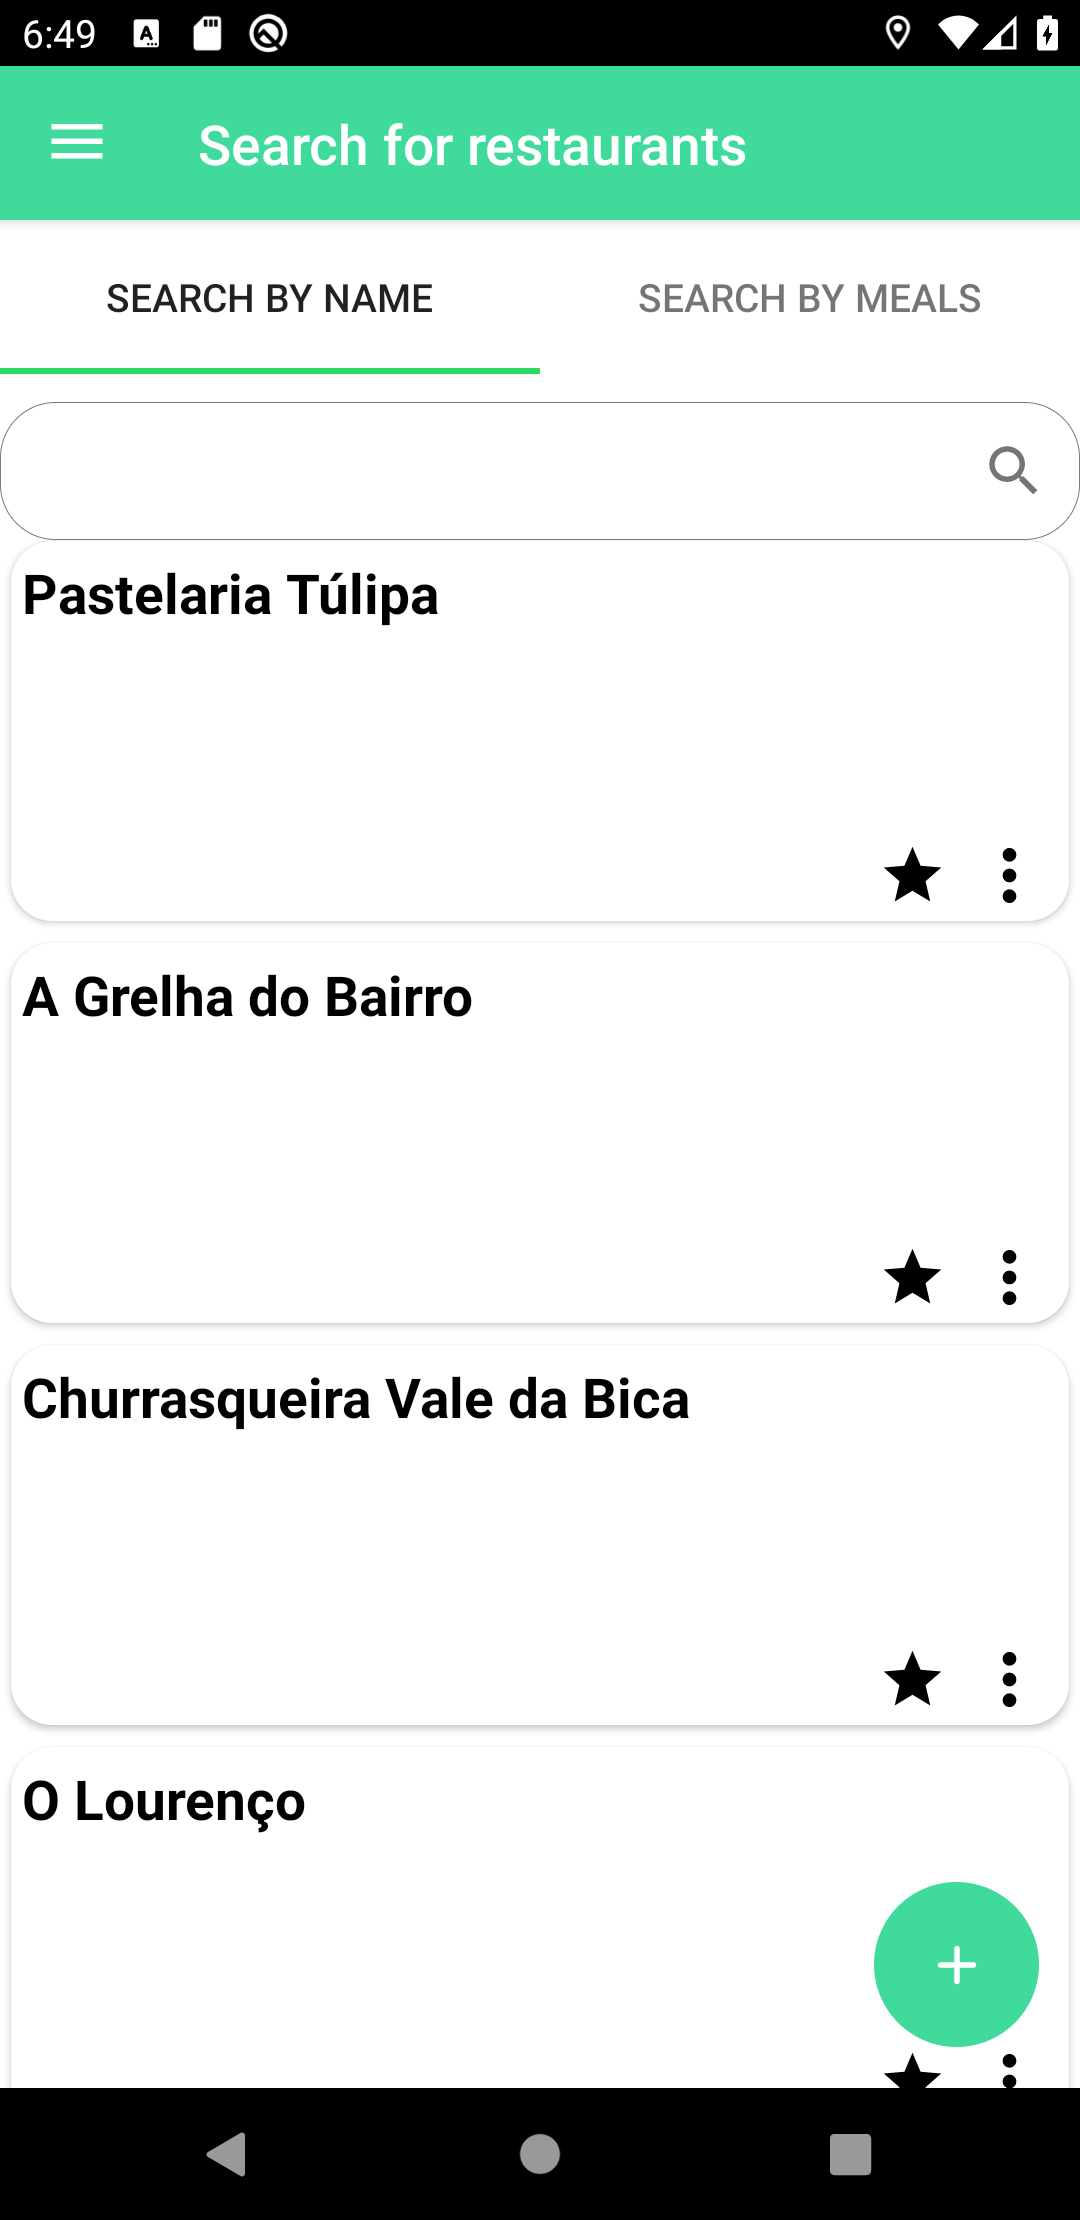
\includegraphics[scale=0.1, width=\textwidth]{_figures/restaurants_by_name.png}
            \caption{Restaurants by location} 
        \end{subfigure}
        \begin{subfigure}{.3\textwidth}
            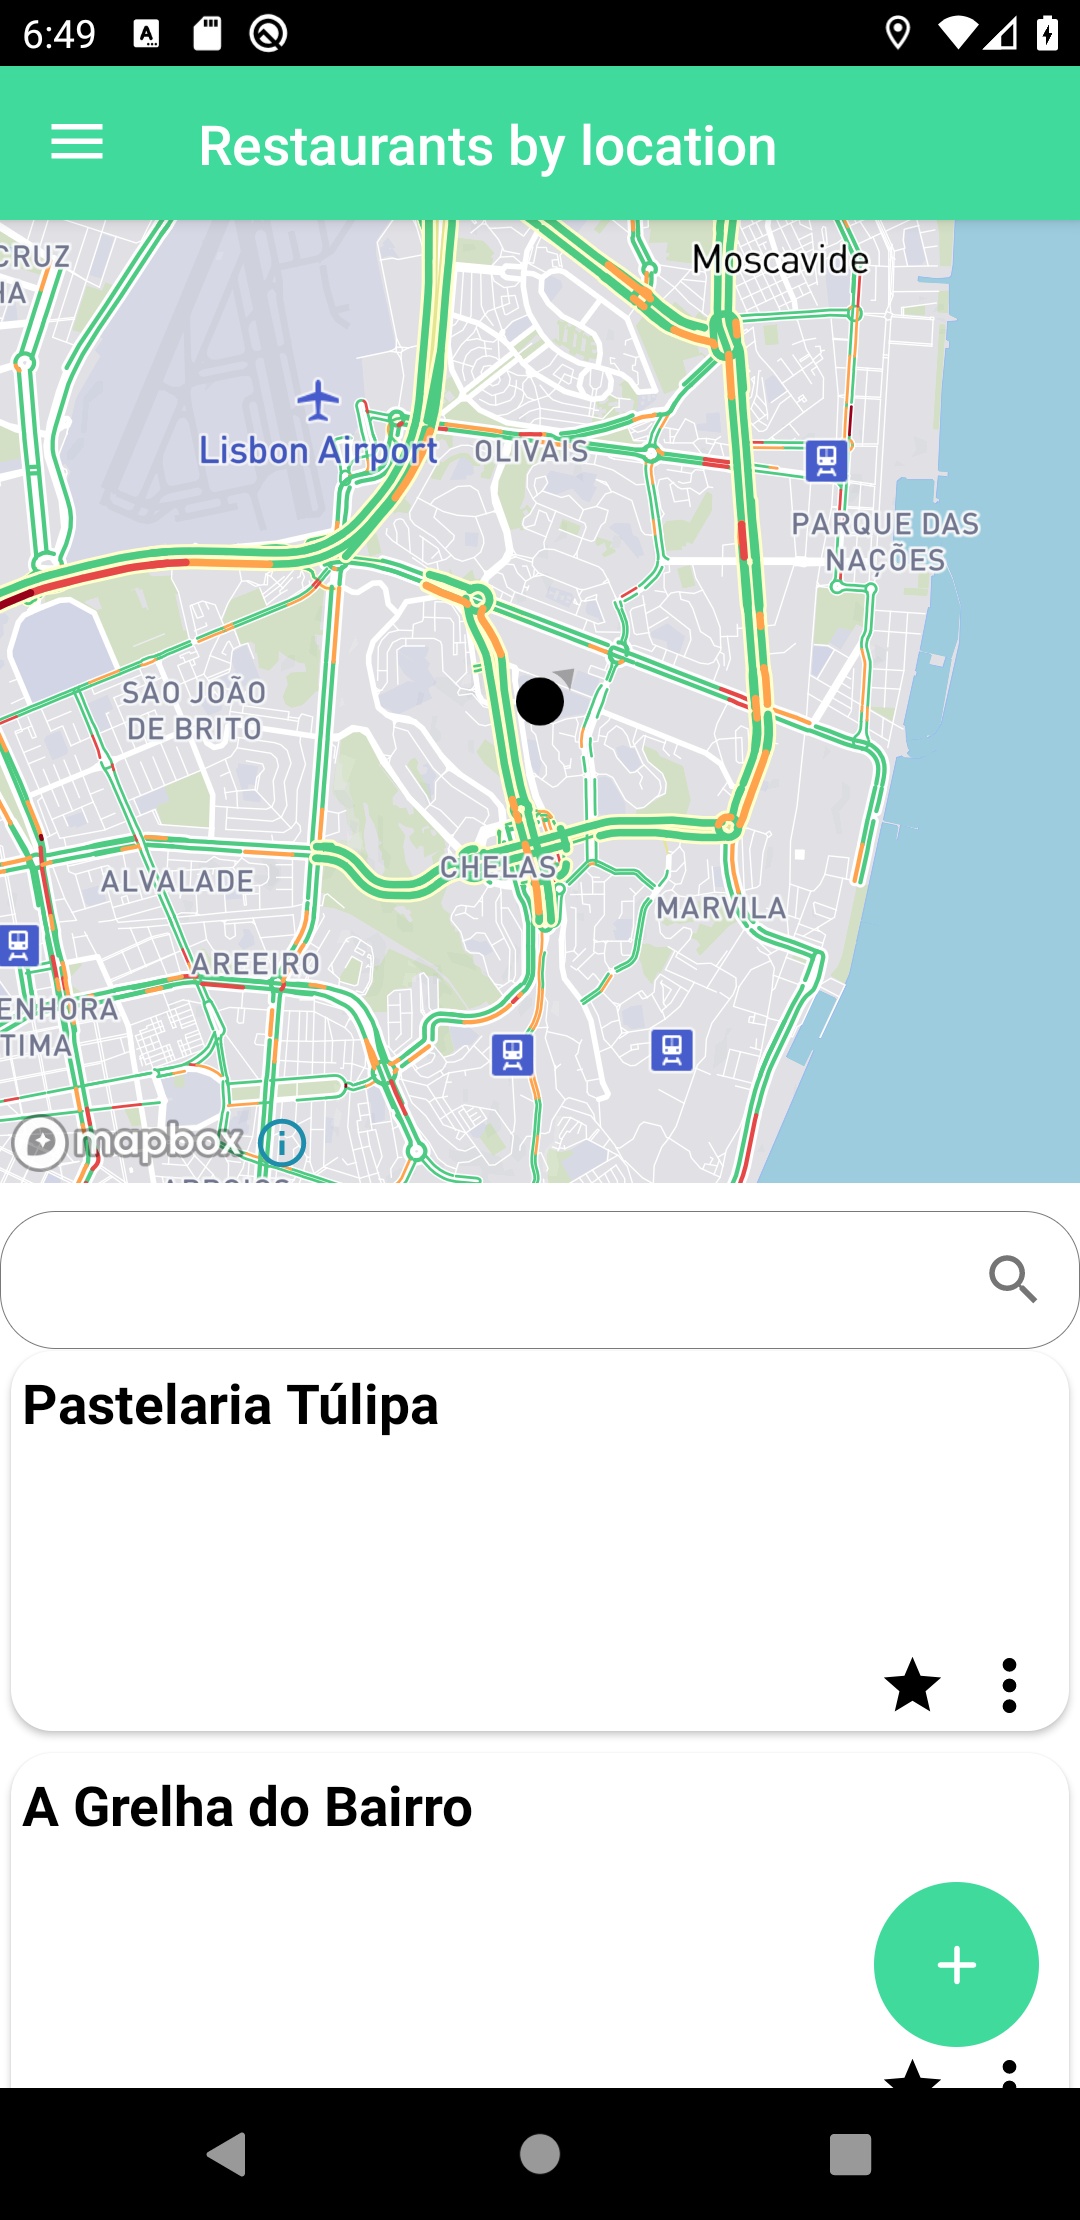
\includegraphics[scale=0.1, width=\textwidth]{_figures/restaurants_map.png}
            \caption{Restaurants by location with map} 
        \end{subfigure}%        
    \end{center}
\end{figure}

Restaurants can also be created by a user and added to a certain location, more specifically the current user's geolocation when 
the restaurant is being created. This can be done by clicking on the plus icon in the images above.\\

When clicking on a restaurant, the user can observe its menu. However if no submissions were made for this restaurant the menu will
be filled with suggested meals from the database, as shown below.\\

\begin{figure}[H]
    \begin{center}
        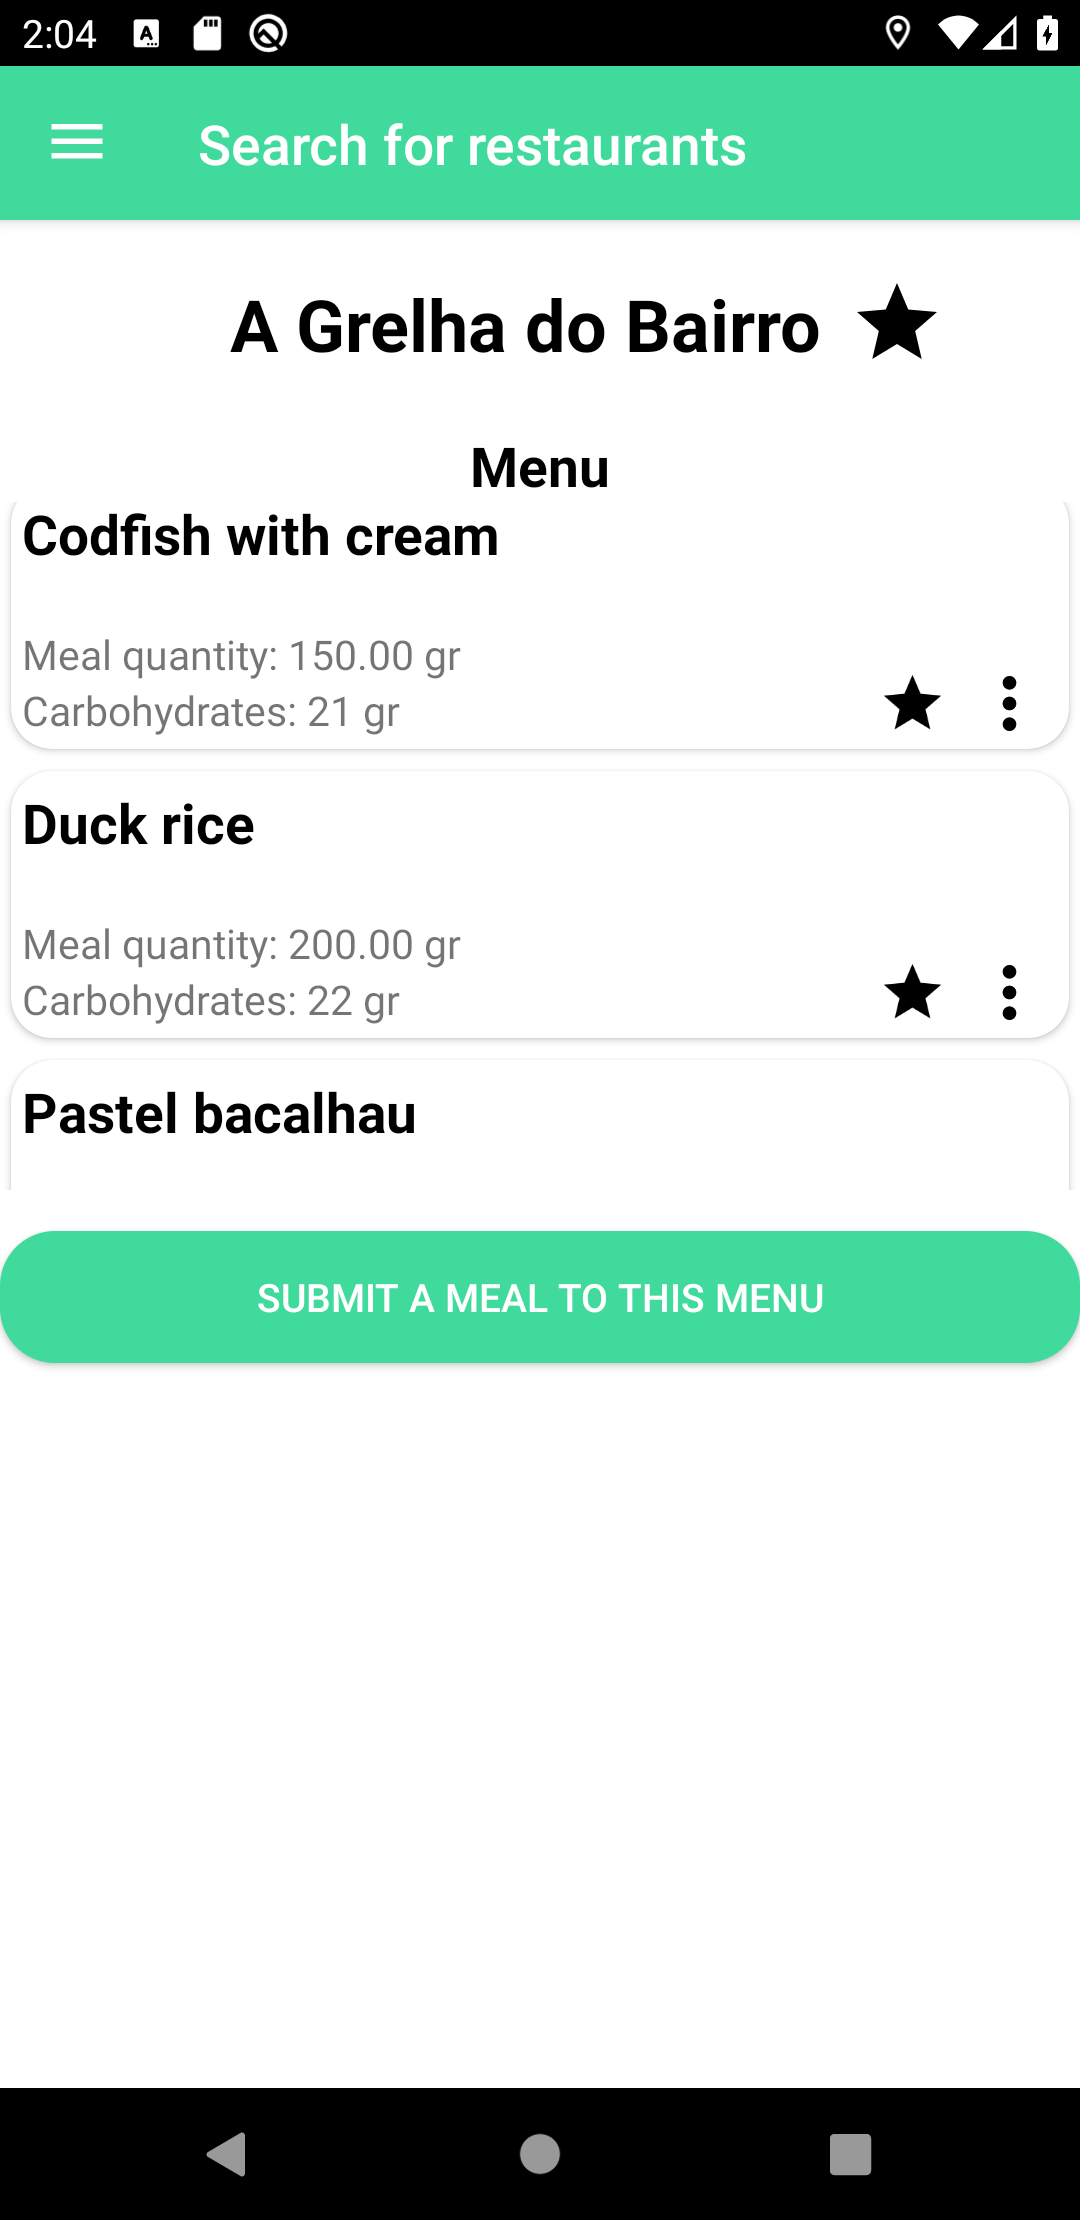
\includegraphics[scale=0.1]{_figures/restaurant_detail.png}
        \caption{Restaurant detail} 
    \end{center}
\end{figure}

If a meal that exist in the restaurant's menu is not present in this list, the user can add it by clicking on the 
'submit a meal for this menu' button.\\

If a certain meal in this list exist in the restaurant's menu, the user can add a portion by clicking on the meal inside the list
and following this procedure:\\

\begin{figure}[H]
    \captionsetup[subfigure]{justification=centering}
    \begin{center}
        \begin{subfigure}{.3\textwidth}
            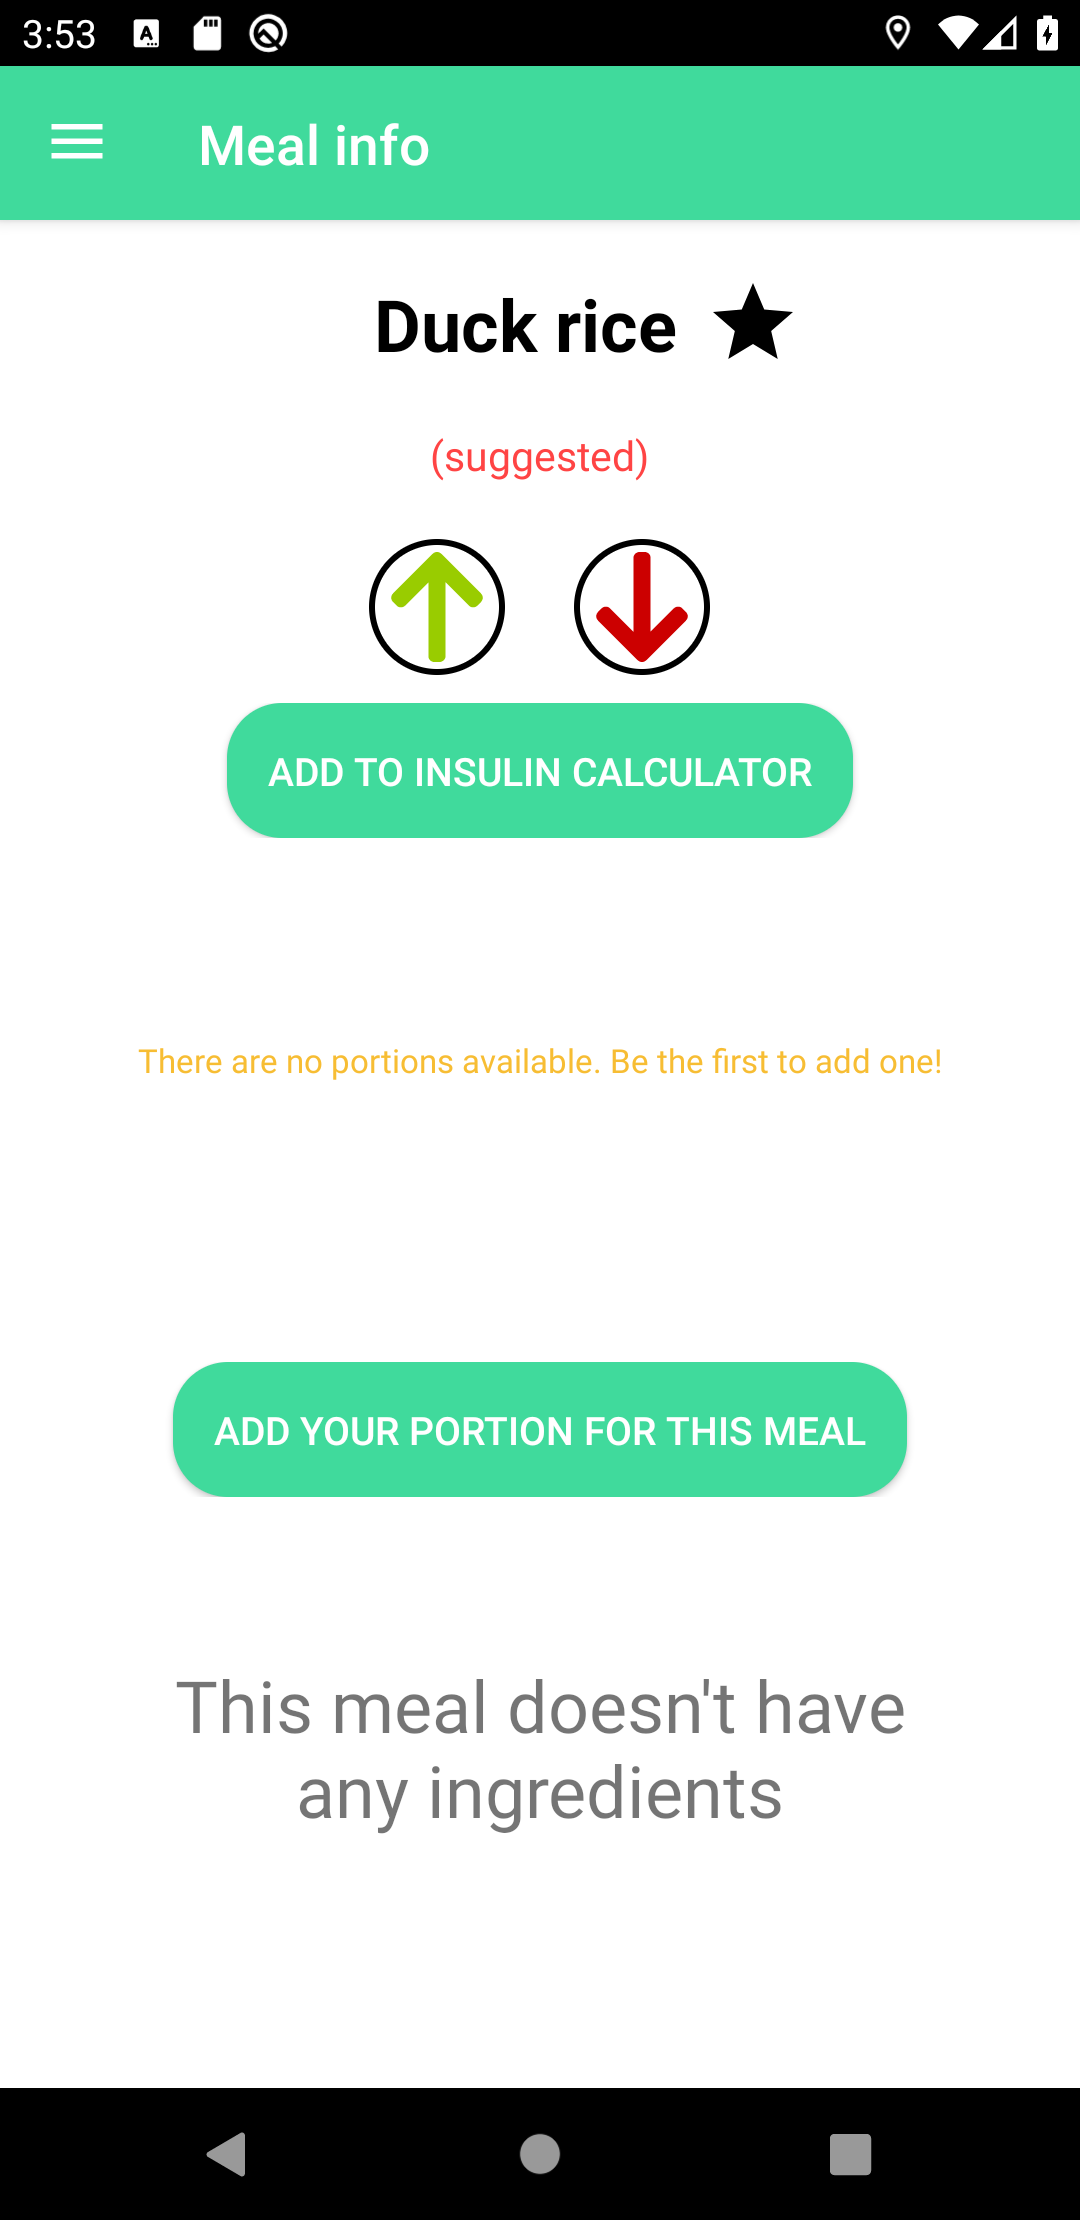
\includegraphics[scale=0.1, width=\textwidth]{_figures/meal_detail.png}
            \caption{Meal detail} 
        \end{subfigure}
        \begin{subfigure}{.3\textwidth}
            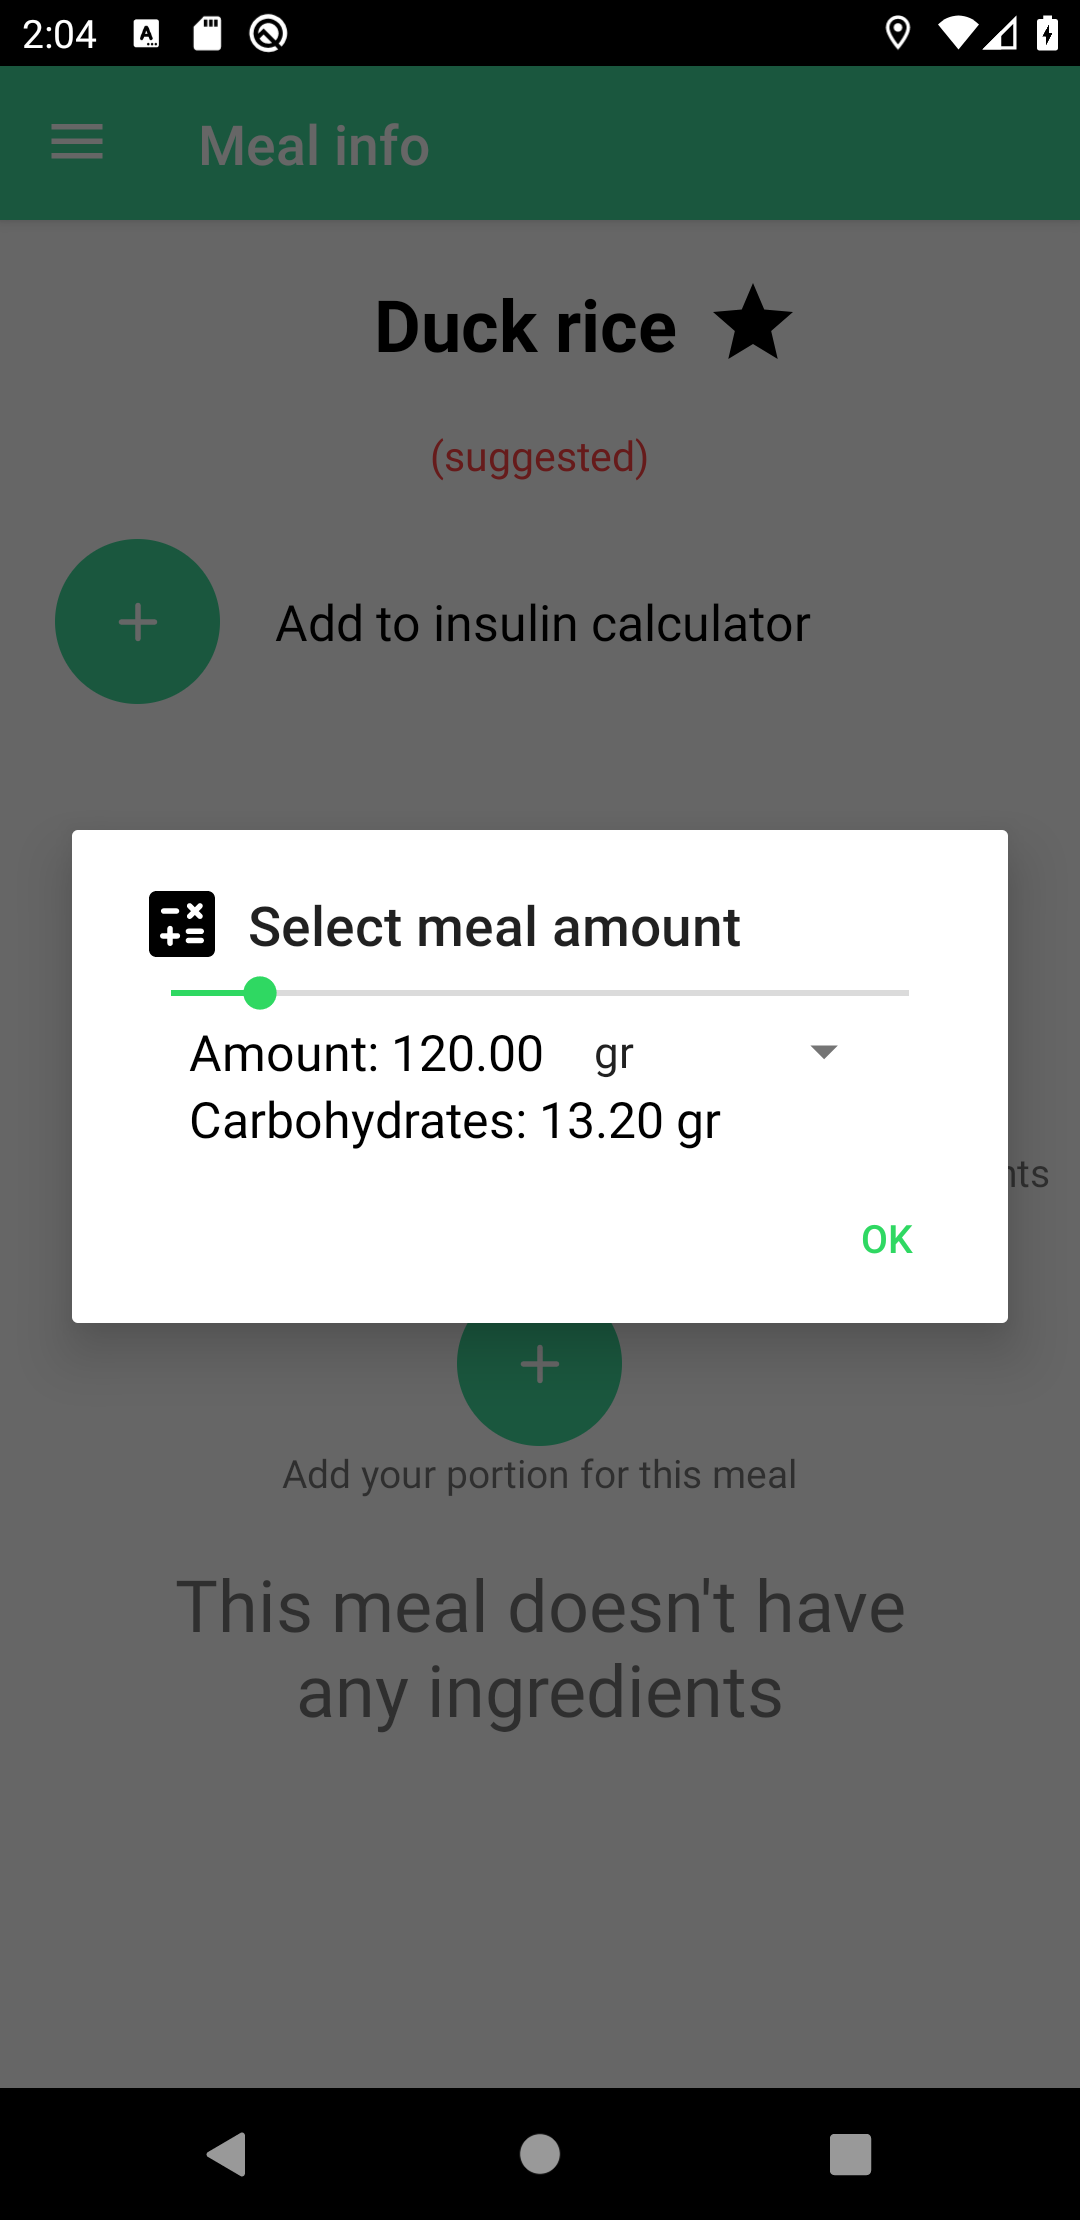
\includegraphics[scale=0.1, width=\textwidth]{_figures/add_portion.png}
            \caption{Adding a portion for this meal} 
        \end{subfigure}%        
        \begin{subfigure}{.3\textwidth}
            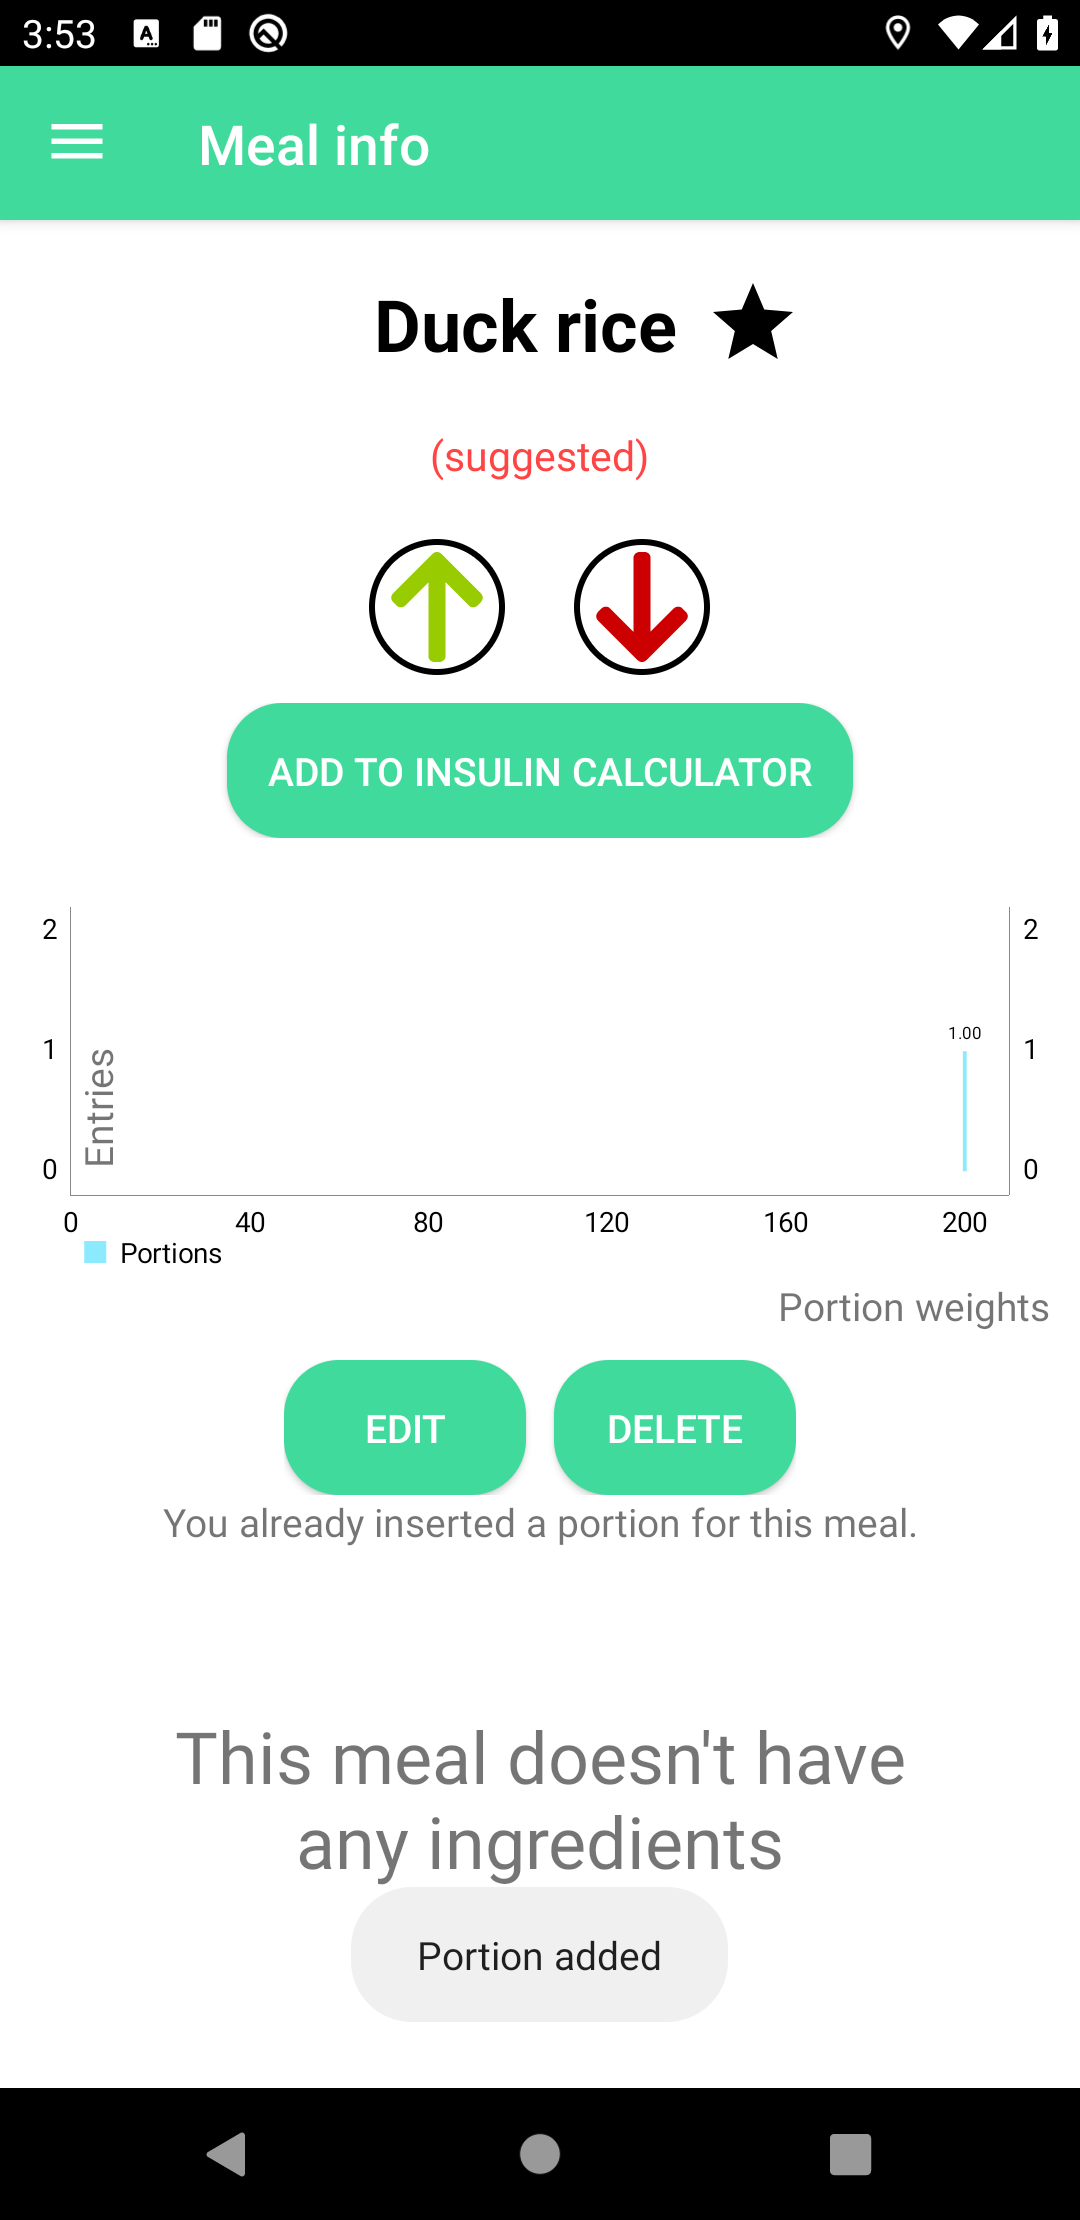
\includegraphics[scale=0.1, width=\textwidth]{_figures/portion_added.png}
            \caption{Portion added with graph showing the result} 
        \end{subfigure}%        
    \end{center}
\end{figure}

The user can also access available meals by accessing 'By name' inside the Meals box, which will display a tab menu with the
platform's suggested meals and meals' ingredients.\\

\begin{figure}[H]
    \captionsetup[subfigure]{justification=centering}
    \begin{center}
        \begin{subfigure}{.3\textwidth}
            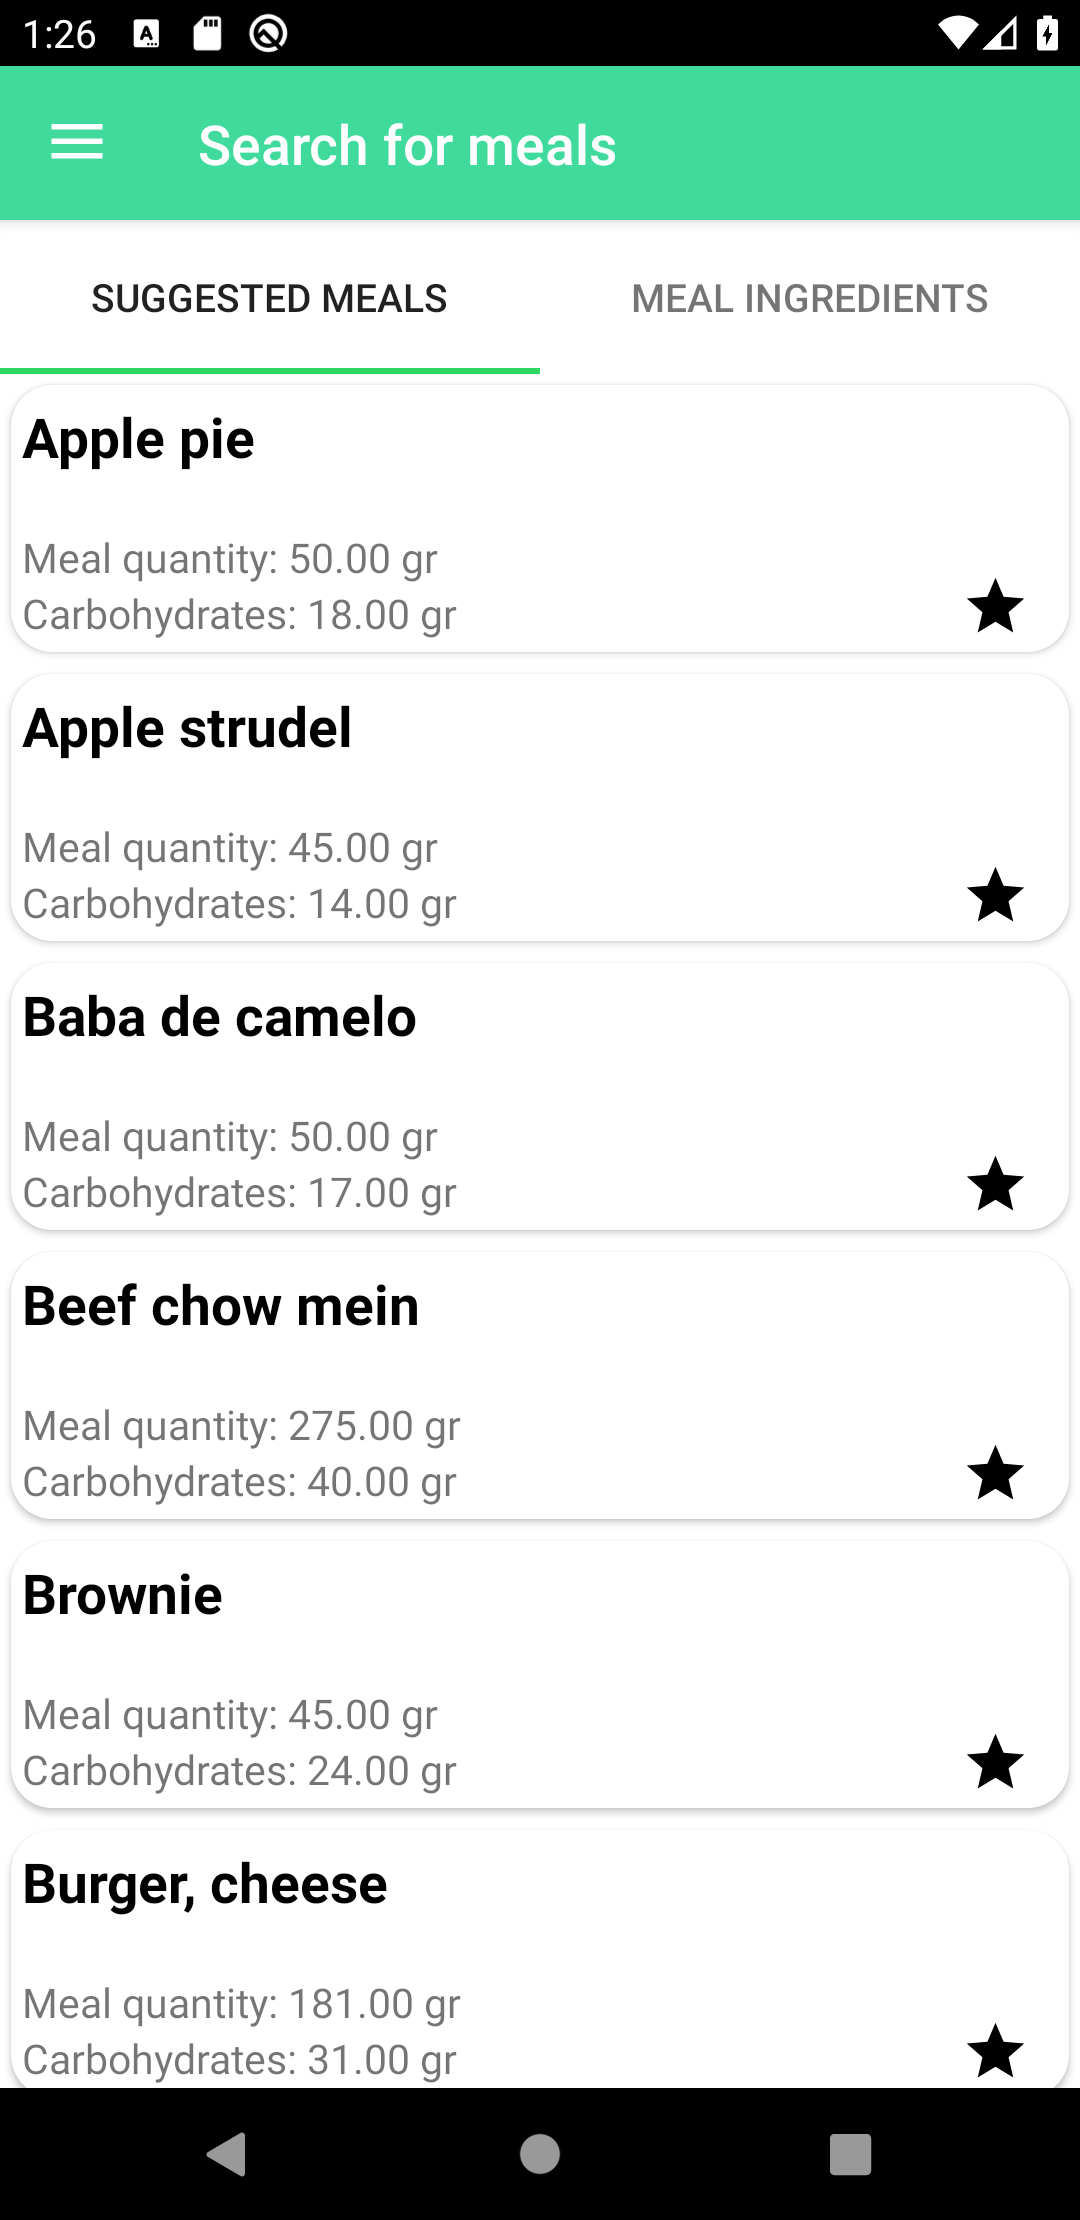
\includegraphics[scale=0.1, width=\textwidth]{_figures/suggested_meals.png}
            \caption{Suggested meals list} 
        \end{subfigure}
        \begin{subfigure}{.3\textwidth}
            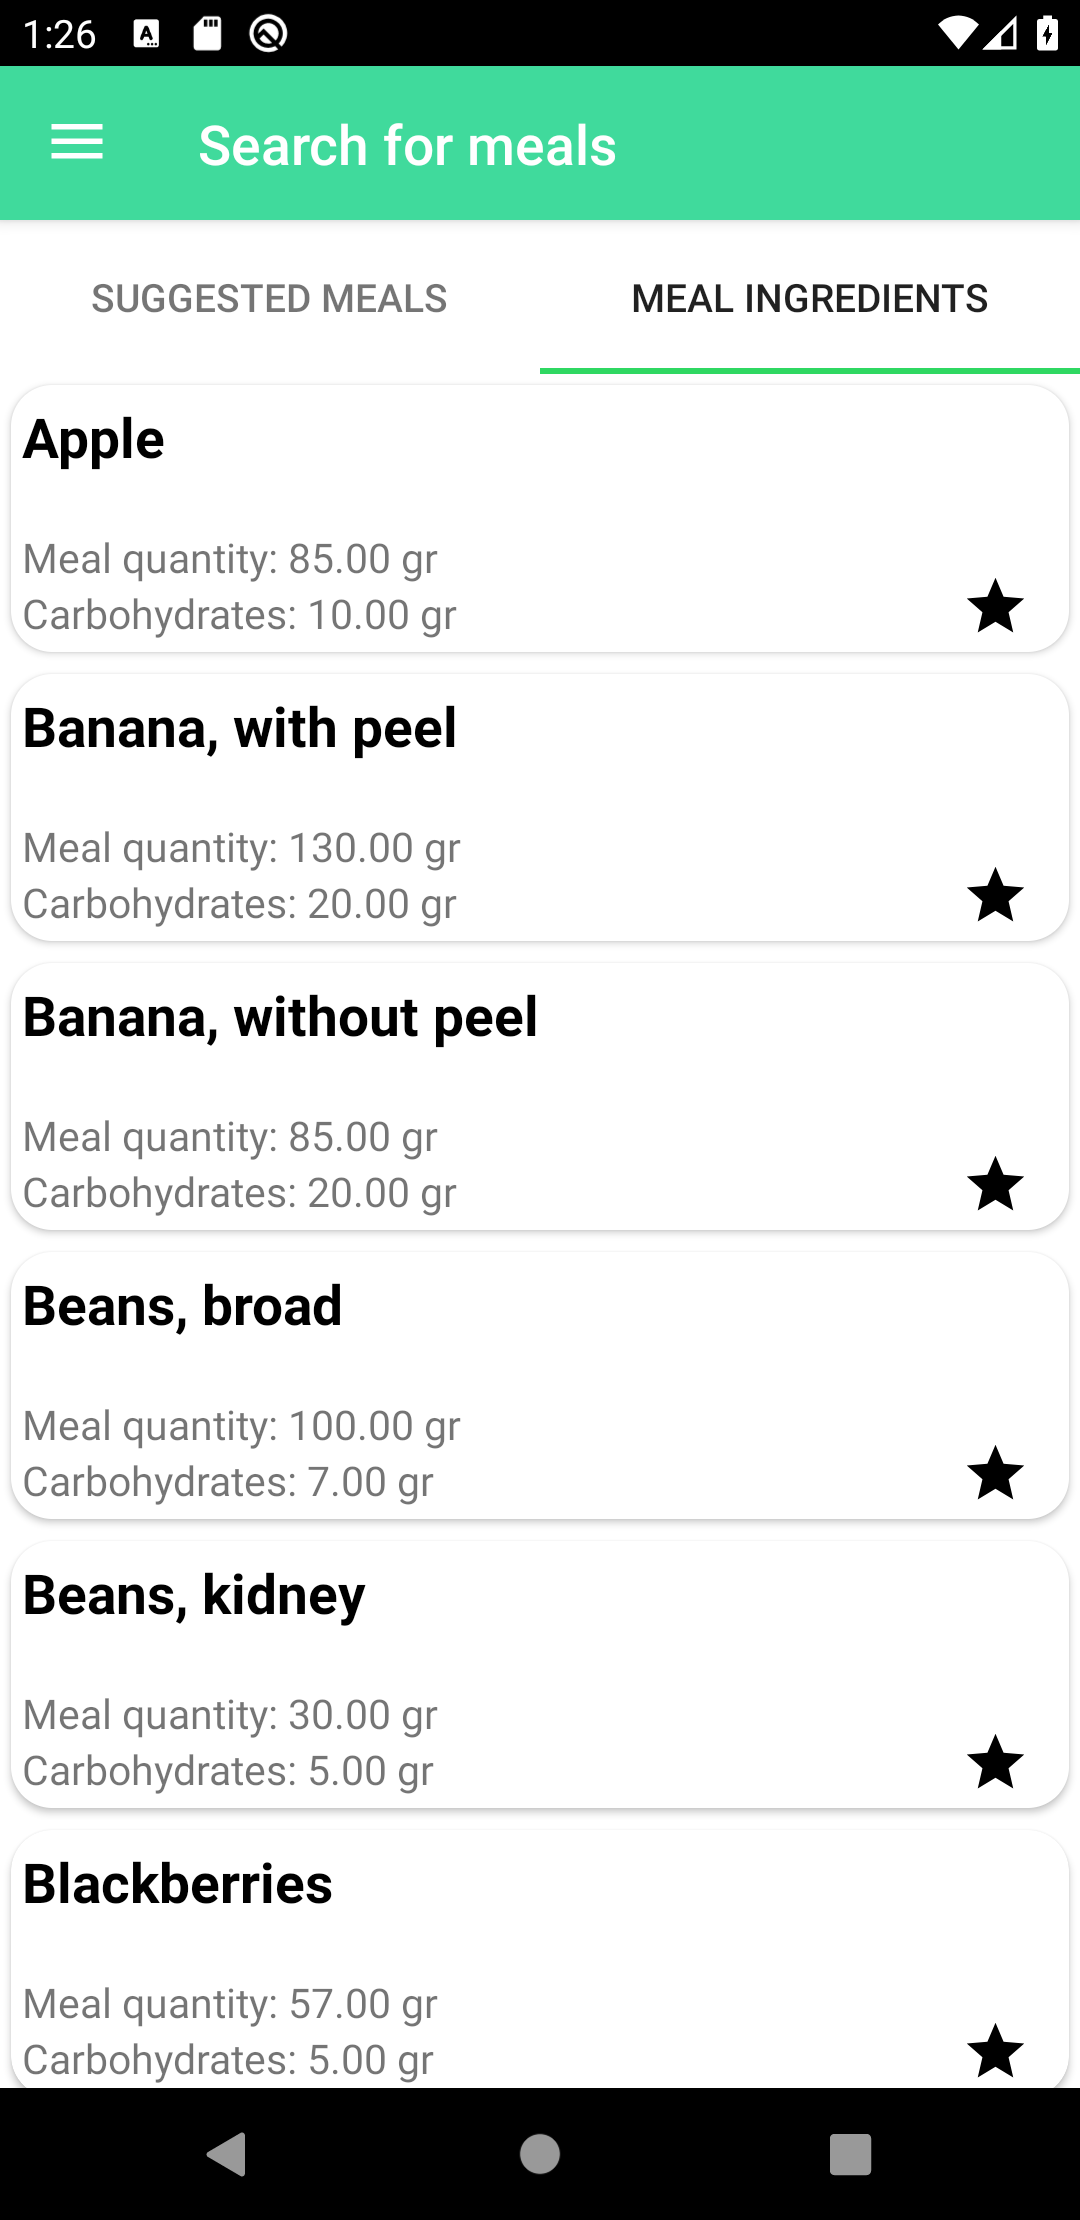
\includegraphics[scale=0.1, width=\textwidth]{_figures/meal_ingredients.png}
            \caption{Meal ingredients list} 
        \end{subfigure}%        
    \end{center}
\end{figure}

\subsubsection{Creating custom meals}

\begin{figure}[H]
    \captionsetup[subfigure]{justification=centering}
    \begin{center}
        \begin{subfigure}{.3\textwidth}
            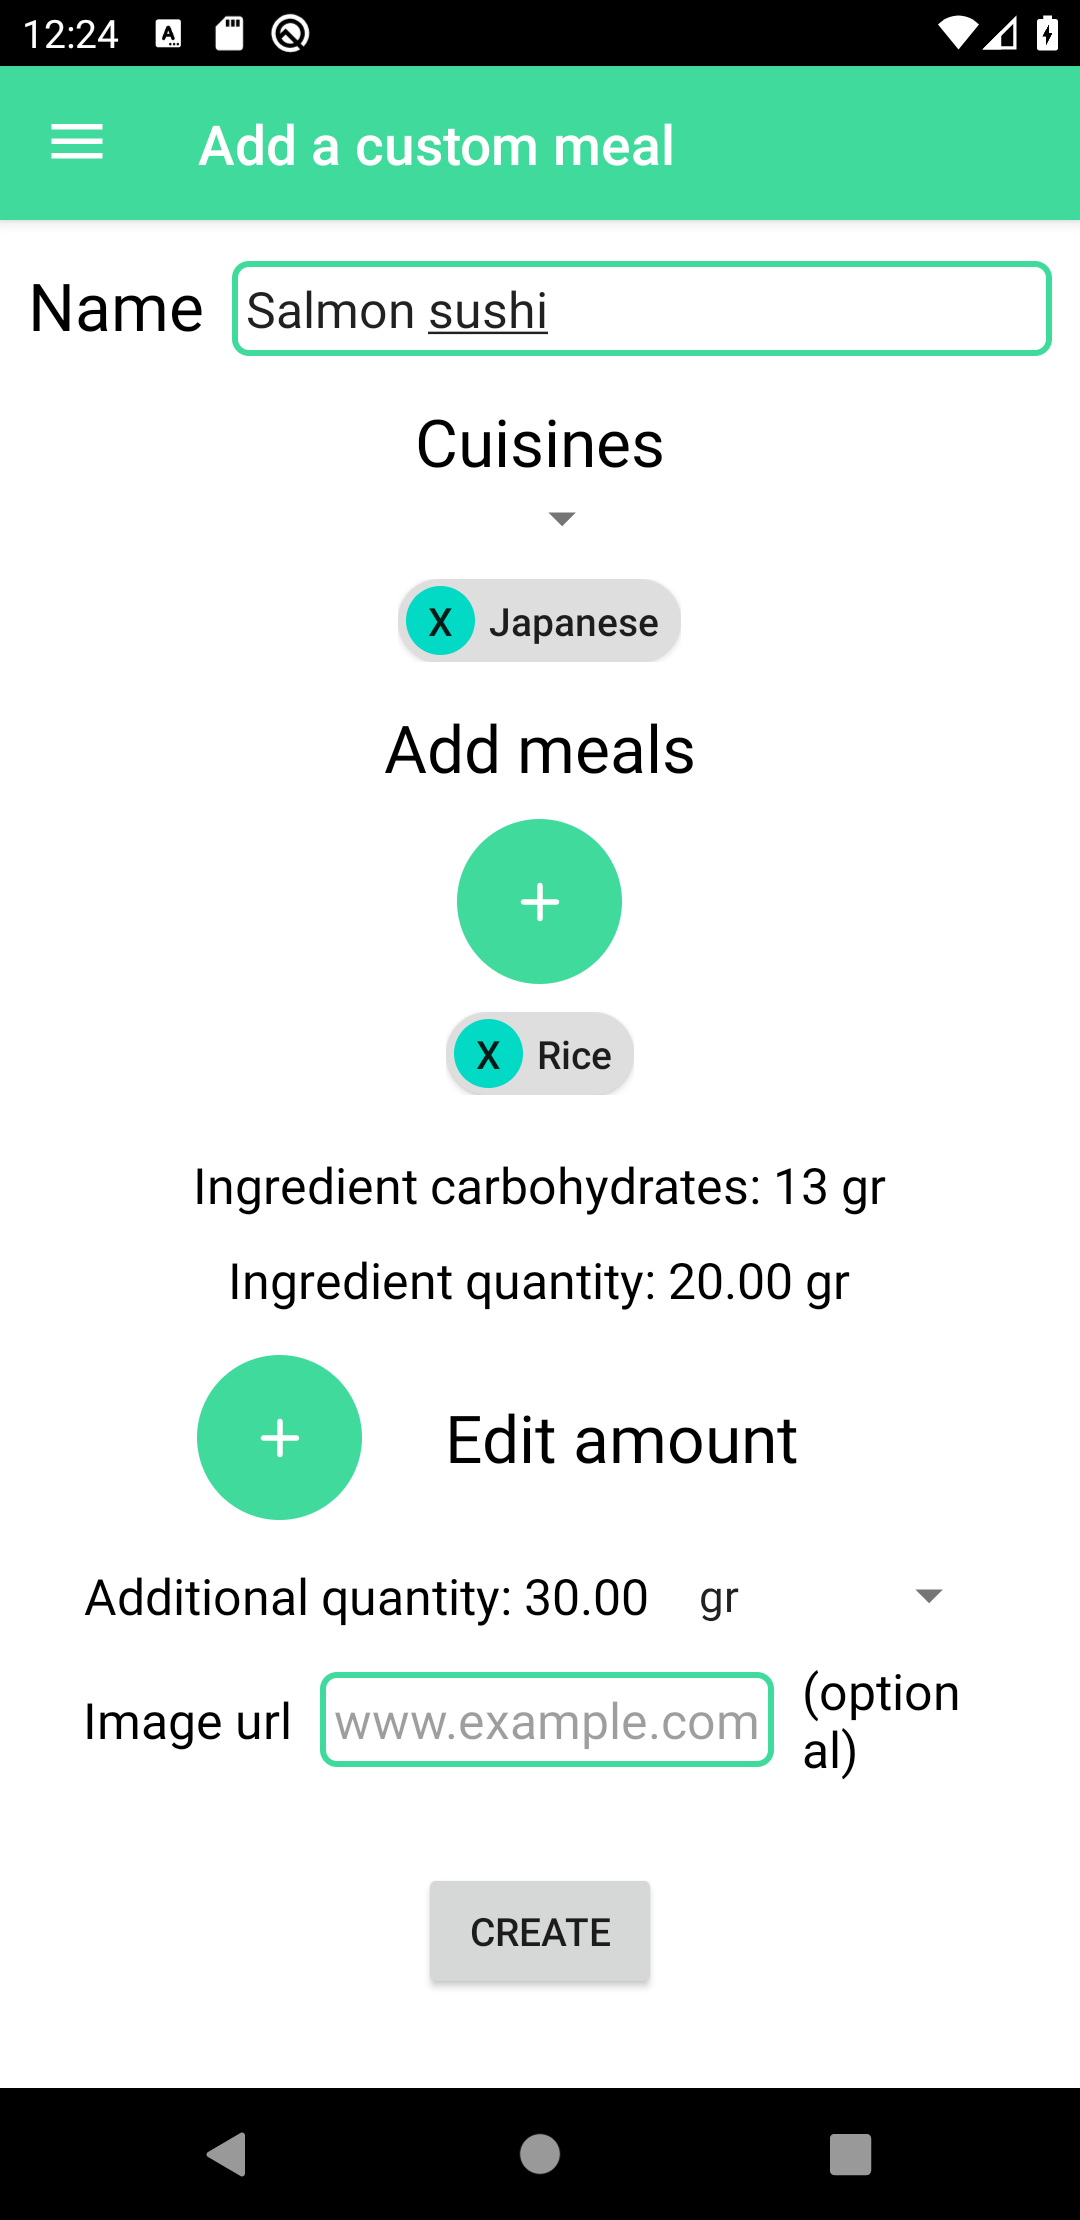
\includegraphics[scale=0.1, width=\textwidth]{_figures/create_custom_meal.png}
            \caption{Custom meal creation} 
        \end{subfigure}
        \begin{subfigure}{.3\textwidth}
            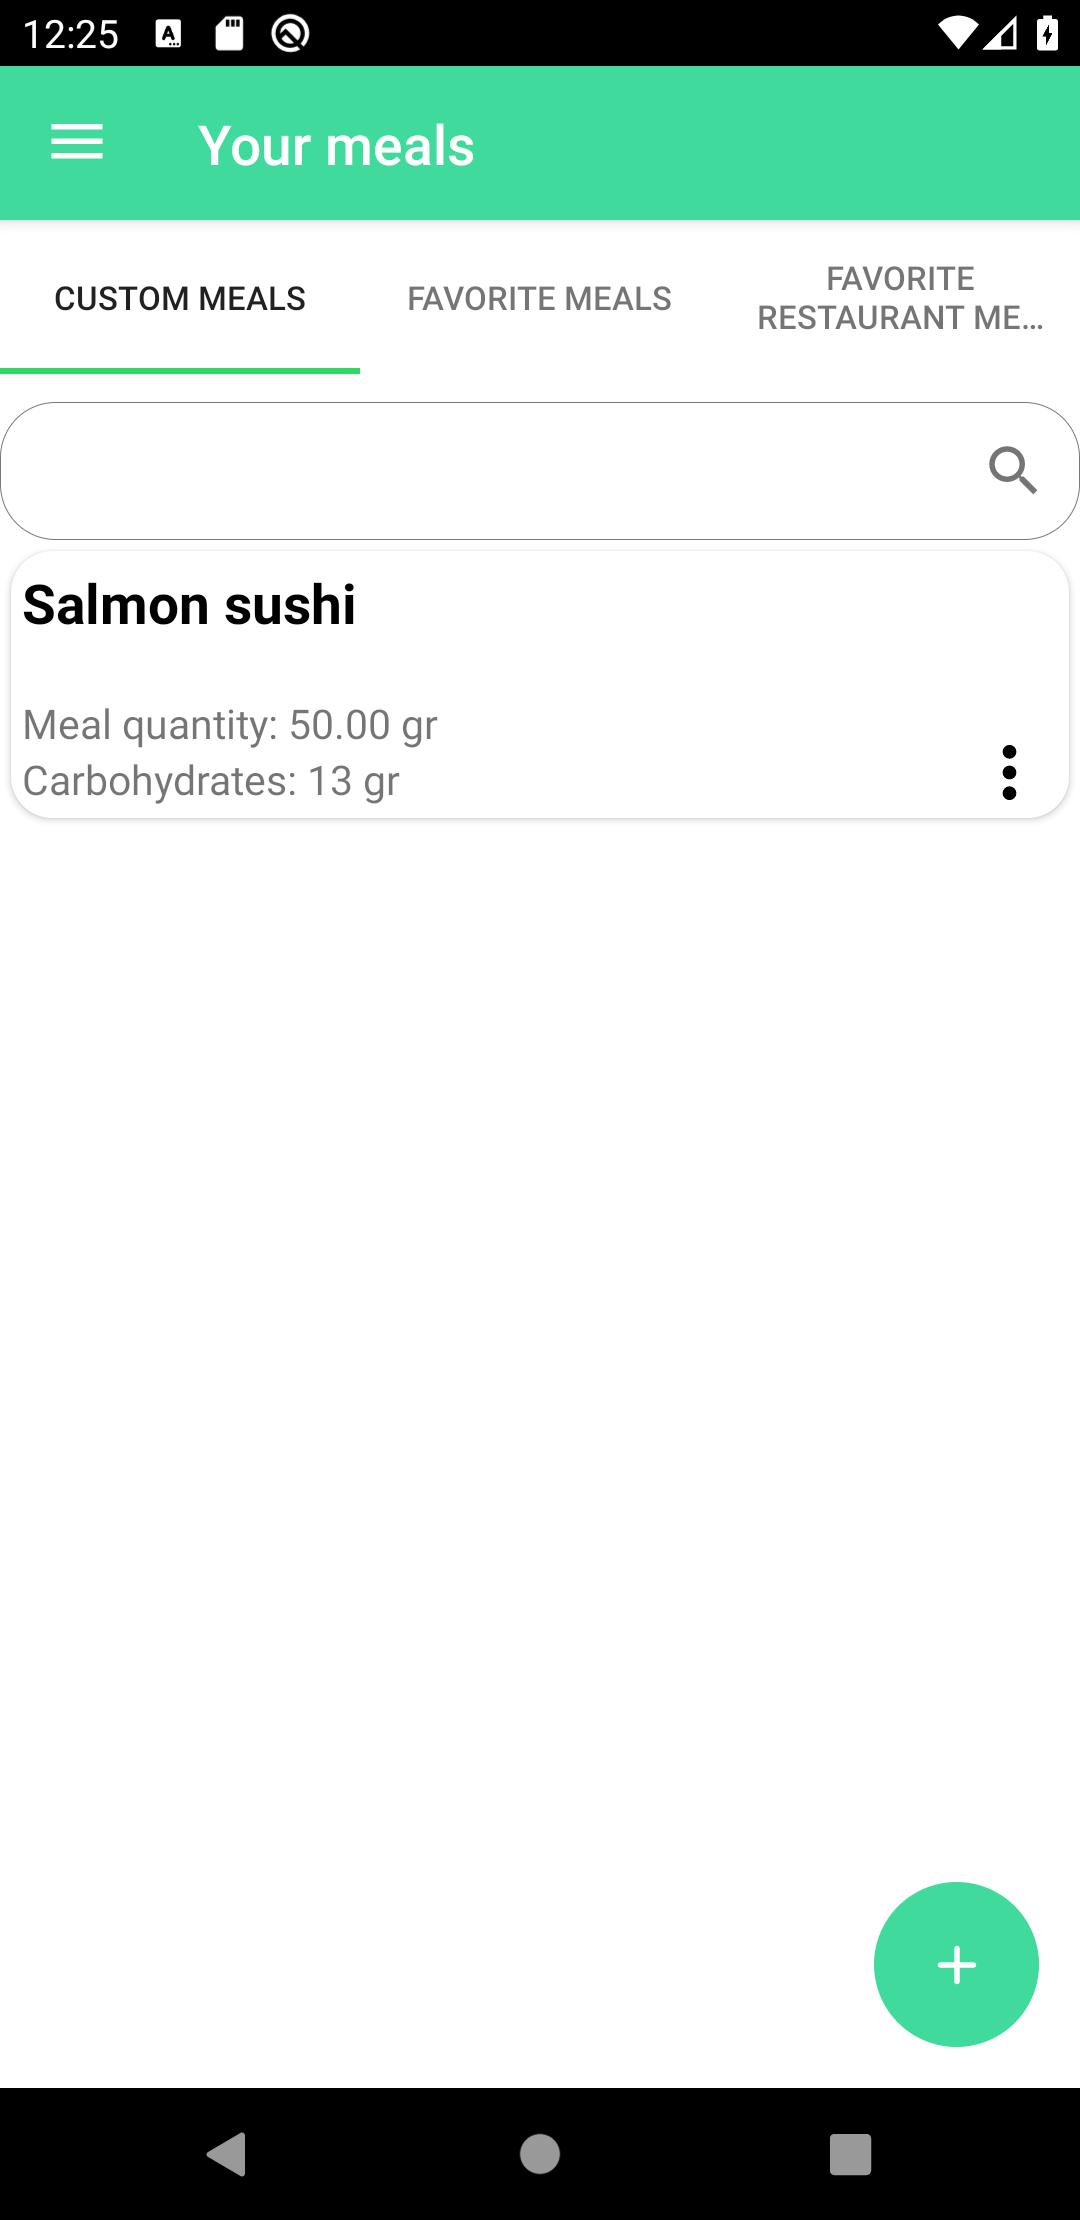
\includegraphics[scale=0.1, width=\textwidth]{_figures/custom_meal_after_creation.png}
            \caption{List to access custom meals} 
        \end{subfigure}%        
    \end{center}
\end{figure}

As seen above, the user can create custom meals in order to add to a restaurant menu later or to use it 
with the insulin calculator, which will be explained in the next section.

\subsubsection{Using the insulin calculator}

To use this feature, the user must create at least one insulin profile which time period matches the current time. If the user does not have a valid insulin profile for the current
time, the profile information in this fragment will appear with blank fields.\\

\begin{figure}[H]
    \captionsetup[subfigure]{justification=centering}
    \begin{center}
        \begin{subfigure}{.3\textwidth}
            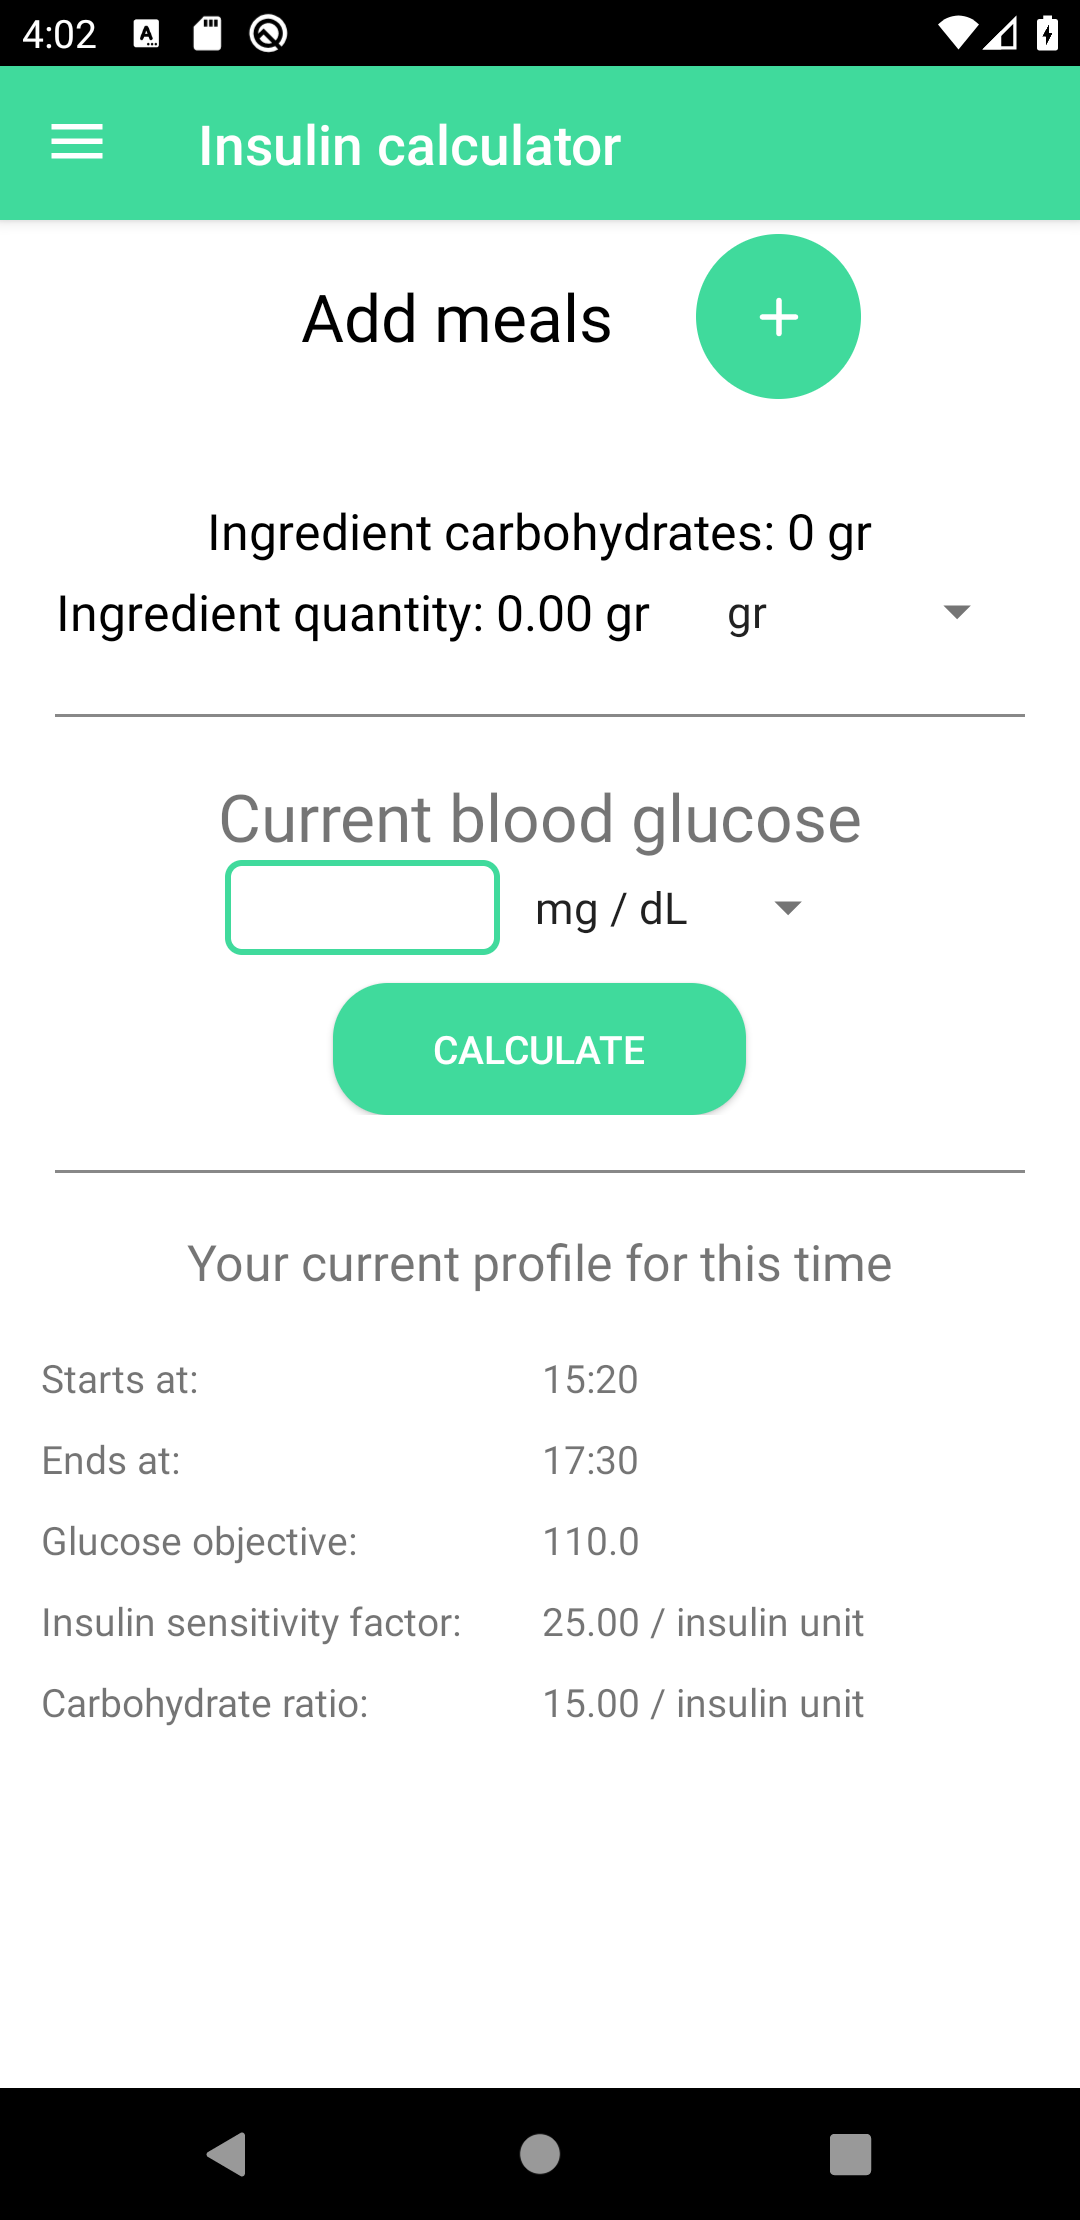
\includegraphics[scale=0.1, width=\textwidth]{_figures/calc_with_profile.png}
            \caption{Calculator with valid profile} 
        \end{subfigure}
        \begin{subfigure}{.3\textwidth}
            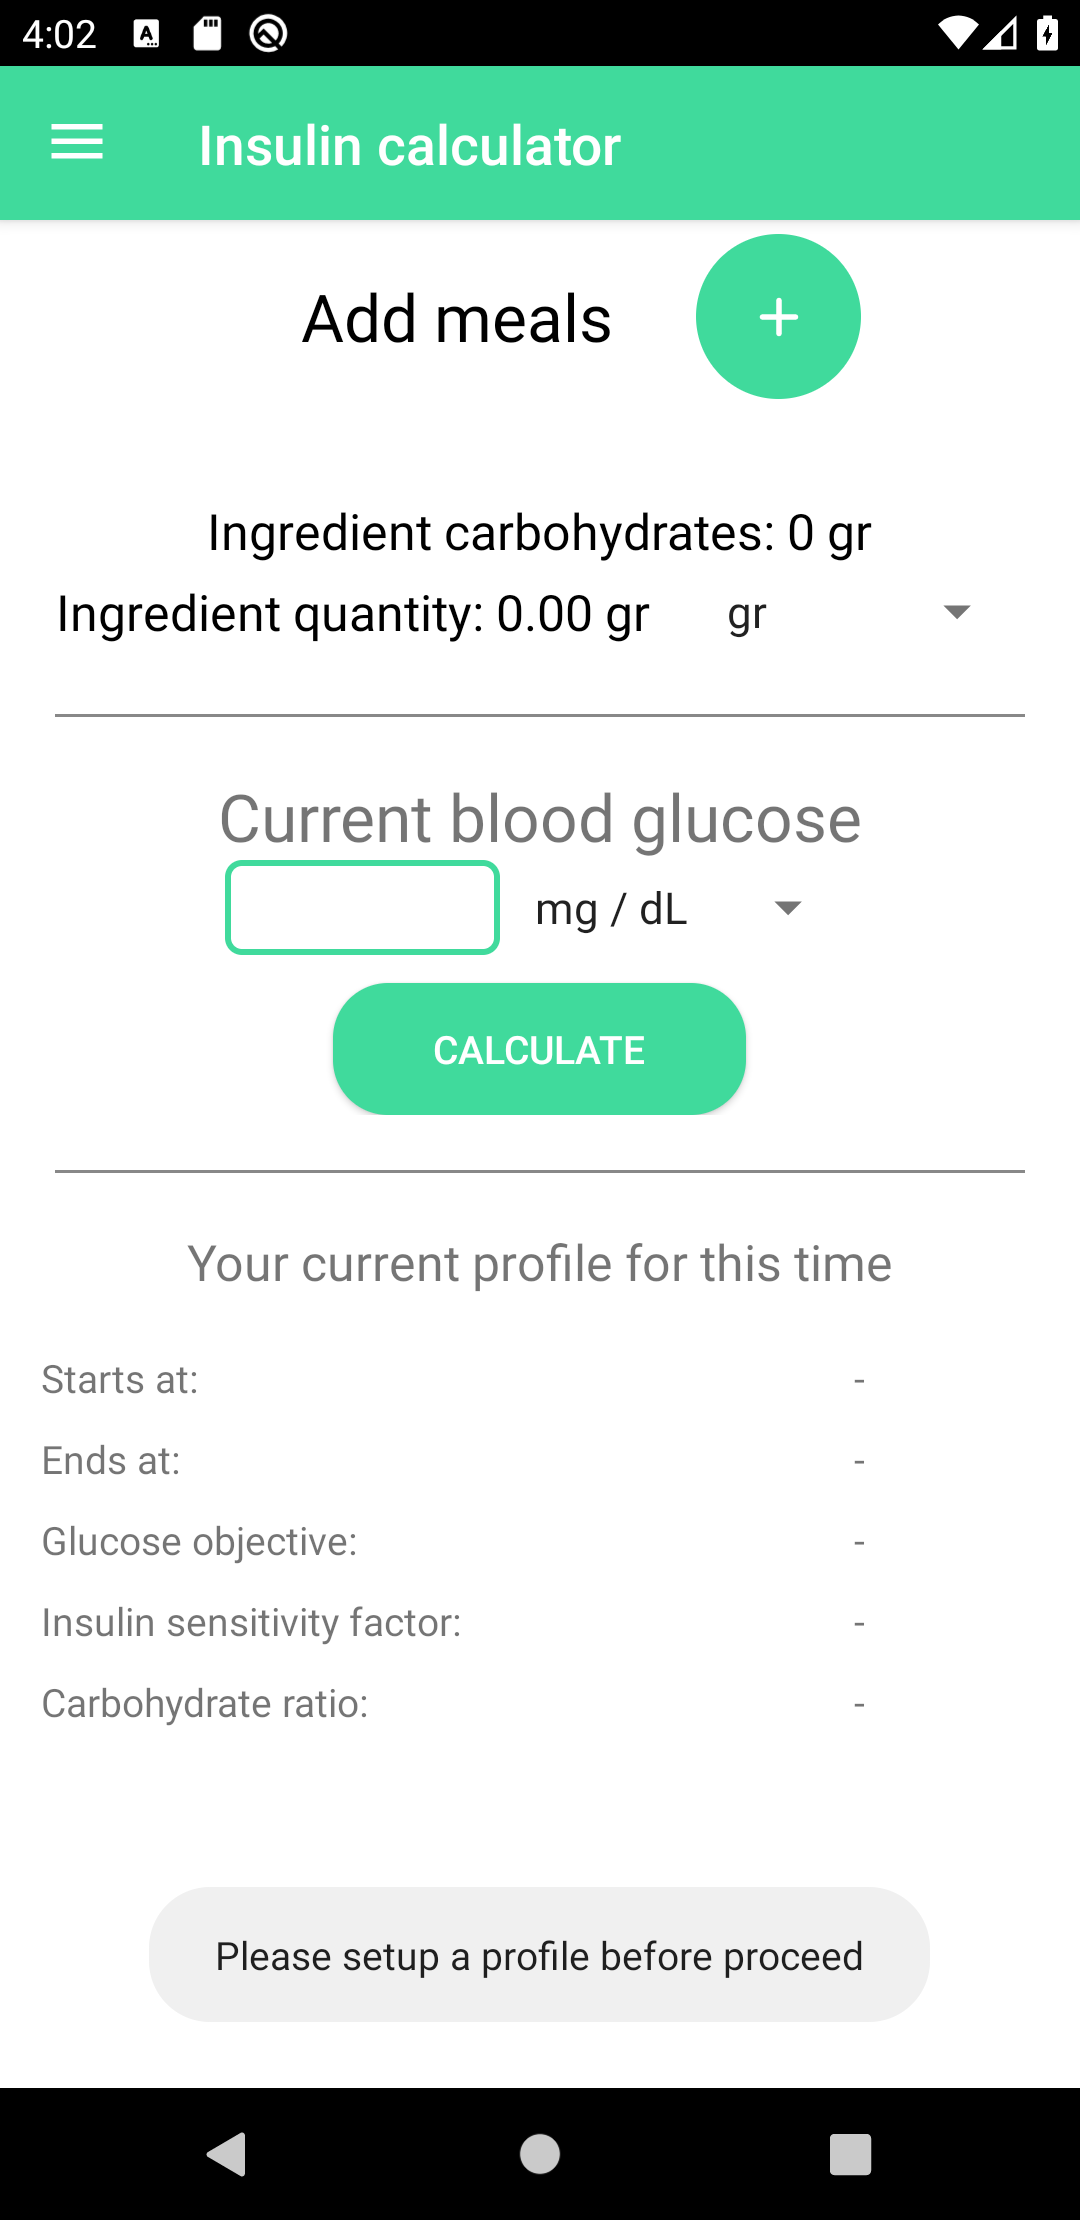
\includegraphics[scale=0.1, width=\textwidth]{_figures/calc_without_profile.png}
            \caption{Calculator without profile} 
        \end{subfigure}%        
    \end{center}
\end{figure}

Having a valid insulin profile, the user must measure its current blood glucose value and select a meal by pressing the plus green button.
When this button is pressed, a tab menu will appear where the user can add:
\begin{itemize}
    \item user's custom meals;
    \item user's favorite meals
    \item ingredients from meals;
    \item suggested meals; 
\end{itemize}

\begin{figure}[H]
    \begin{center}
        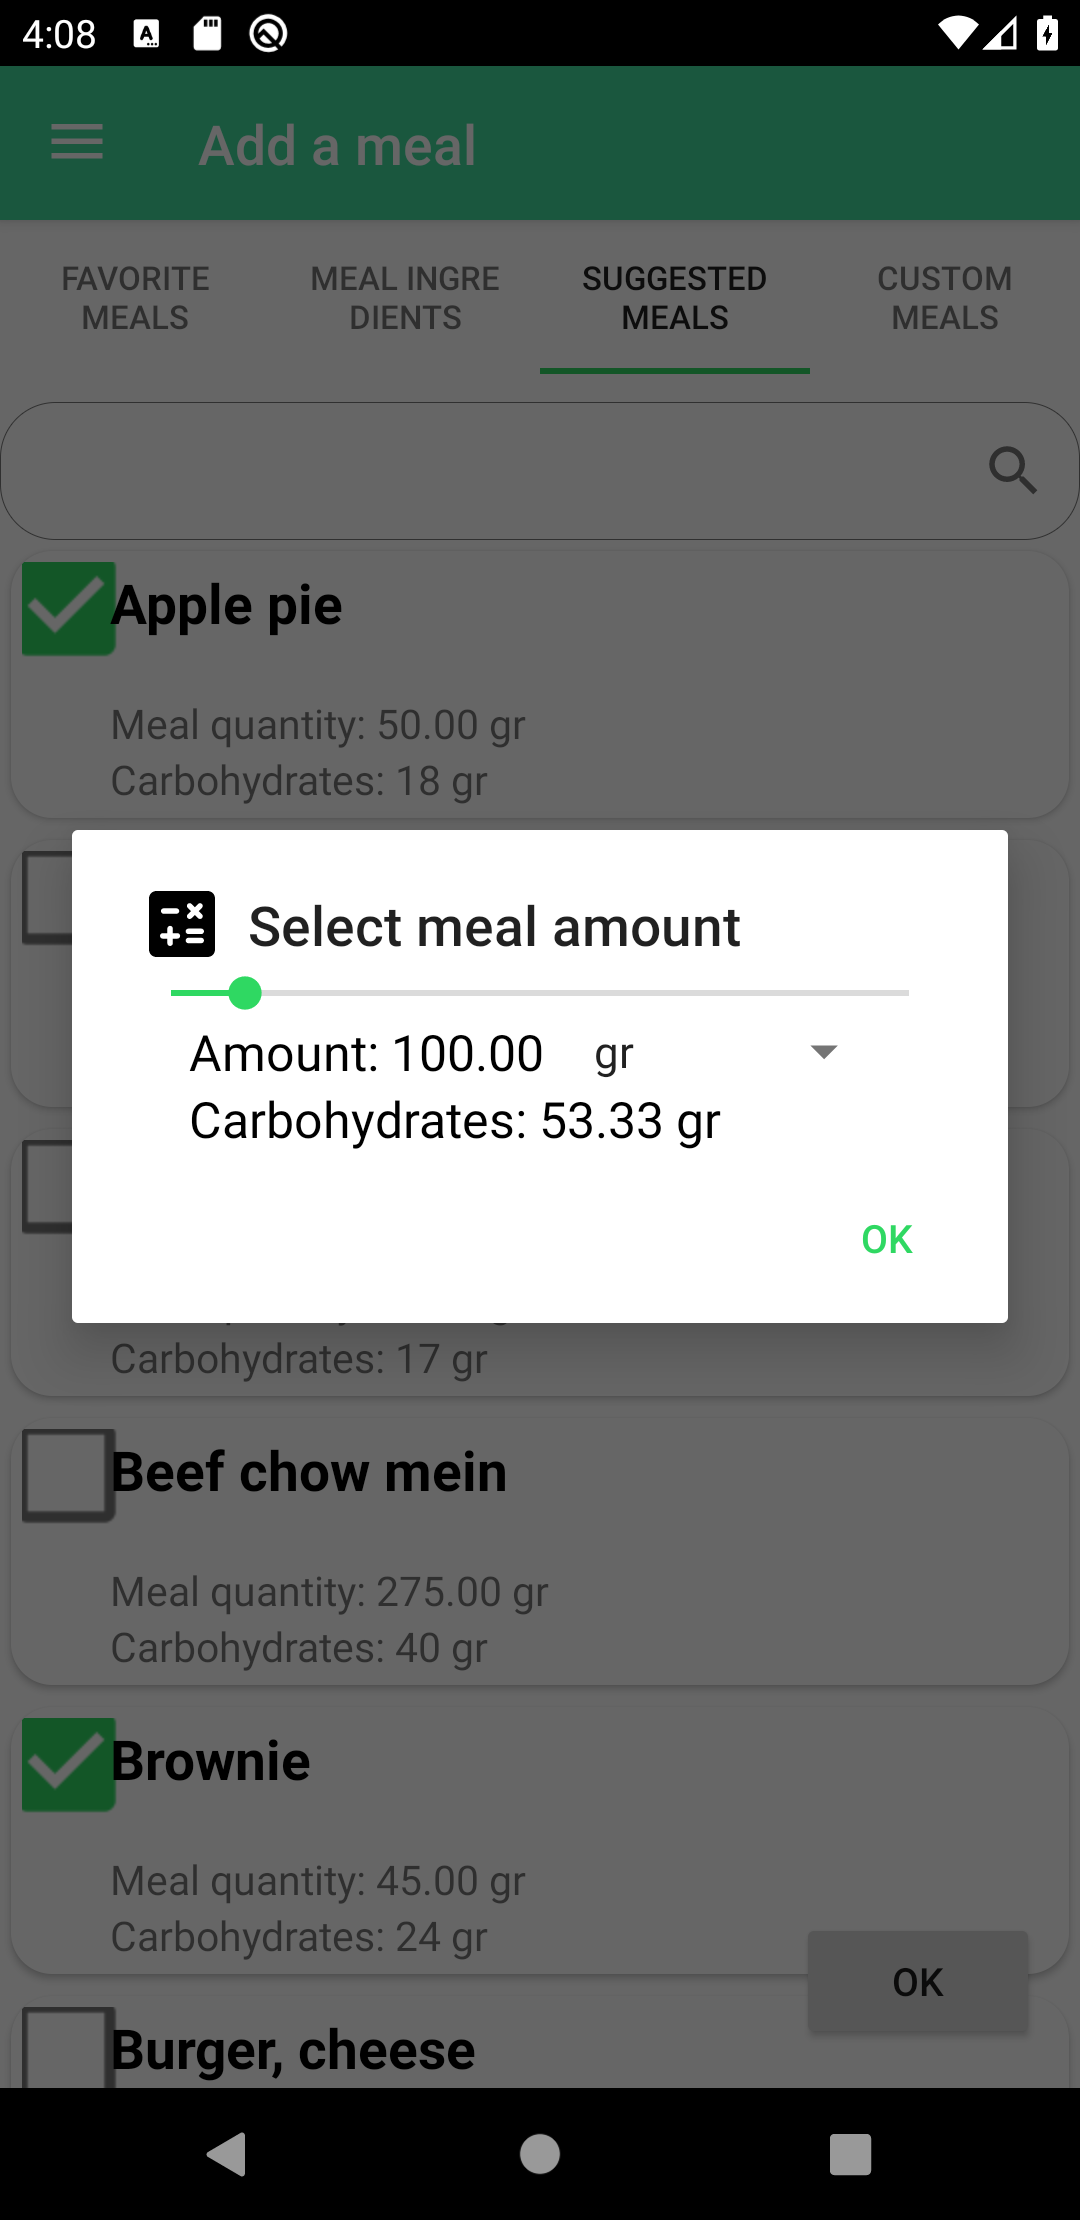
\includegraphics[scale=0.1]{_figures/calc_meal_selection.png}
        \caption{Meal selection menu}
    \end{center}
\end{figure}

After these steps, the user is ready to calculate the insulin dosage that corresponds consuming the select meals, with its current blood glocuse for its current time.

\begin{figure}[H]
    \captionsetup[subfigure]{justification=centering}
    \begin{center}
        \begin{subfigure}{.3\textwidth}
            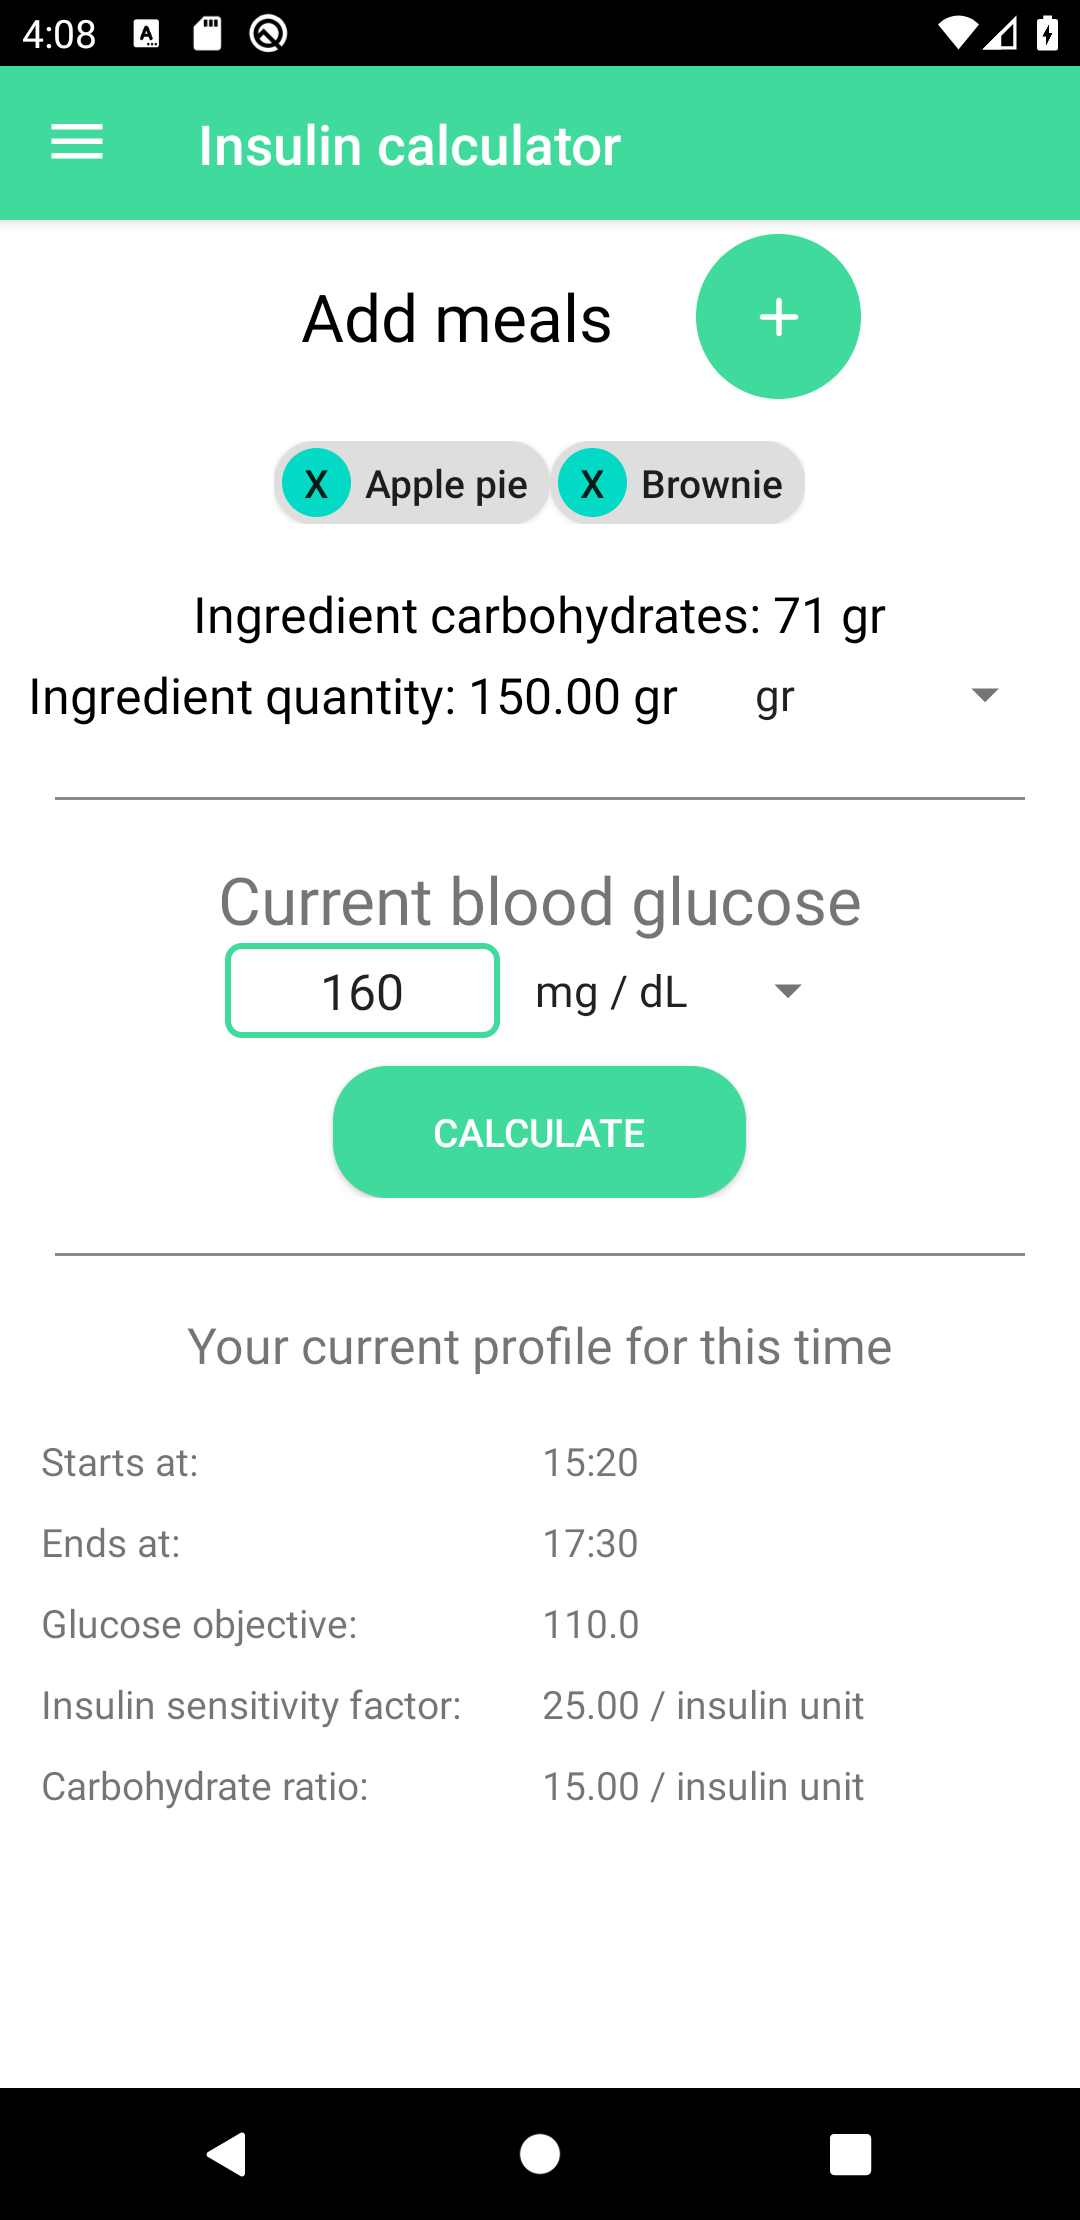
\includegraphics[scale=0.1, width=\textwidth]{_figures/fullfilled_calc.png}
            \caption{Calculator with all the valid field filled} 
        \end{subfigure}
        \begin{subfigure}{.3\textwidth}
            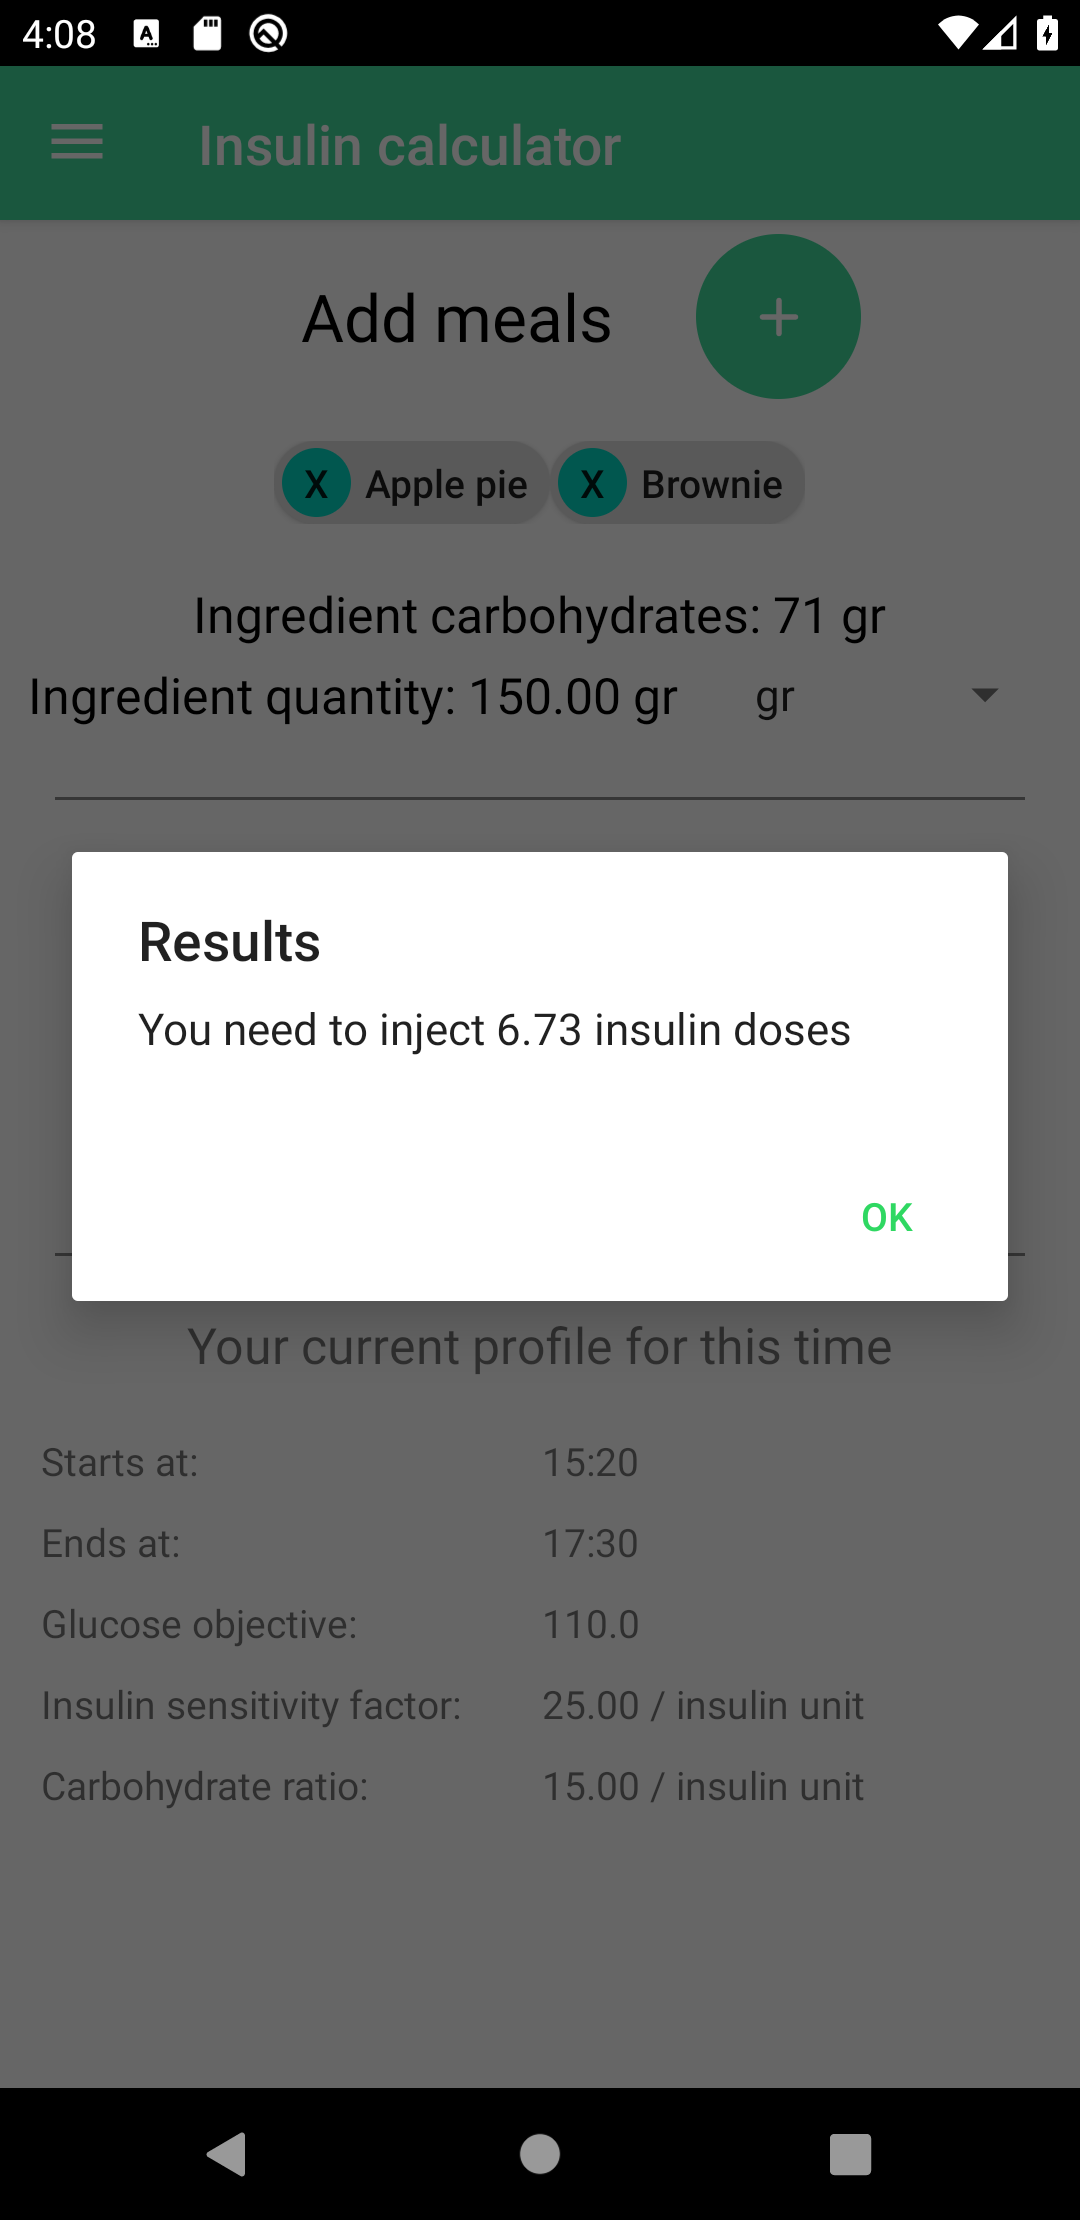
\includegraphics[scale=0.1, width=\textwidth]{_figures/dosage_result.png}
            \caption{Dosage result\\} 
        \end{subfigure}%        
    \end{center}
\end{figure}

\section{Web browser application}

Seeing as the goal of our application is provide nutritional information for meals served in restaurants,
we assumed that a typical user would not search for nearby restaurants on their computer's browser.\\

As such, we decided to develop a minimalist version of our application for browsers with extended moderating functionalities -
an authenticated user can only view and create custom meals and edit their insulin profiles; while a moderator can create suggested ingredients
and meals for cuisines, and view submission reports and act on them, either by banning the submitter, removing the submission or dismissing the report.\\

\subsection{Used tecnologies}

\subsubsection{React framework}

We chose to build the website with JavaScript \cite{javascript} using the React framework \cite{react} , as it was the framework lectured in the Web applications
development course.

\subsubsection{React bootstrap}

We chose to use React Bootstrap not only because it offers tools to quickly build responsive and appealing User Interfaces,
but also because of some familiarity with it due to previous courses such as Internet Programming.\\

Additionally, React Bootstrap was chosen over Bootstrap as it is easy to code due to "each component has been built from scratch
as a true React component, without unneeded dependencies like jQuery." and "each component is implemented with accessibility in mind.
The result is a set of accessible-by-default components, over what is possible from plain Bootstrap."  (from https://react-bootstrap.github.io/)\\


\subsection{Code structure}

\subsubsection{Single-page application}

Regarding design patterns, we decided to develop our web browser application using a Single Page Application approach over
a Multi Page Application. This pattern was chosen as it is faster for the user to navigate after the initial load, allows for
a better user experience and interaction, and it reduces the load on the server, as most resouces (such as HTML and CSS) are
only requested and loaded once by the user.\\

Additionally, React-Router is also used to solve shortcomings that Single Page Applications used to have -
the inability to go back and forth on the browser history without reloading the page and the lack of bookmarking.\\

\subsubsection{Routing}
Bellow is the diagram containing every possible endpoint that can be visited and bookmarked
throughout the application. Green marked endpoints require the user to be authenticated; while red marked ones
require the moderator role to access. When this condition fails the user is met with a "You need to be logged
in to access this resource" message, or with "You need to be a moderator to access this resource!", respectively.

\begin{figure}[H]
    \begin{center}
        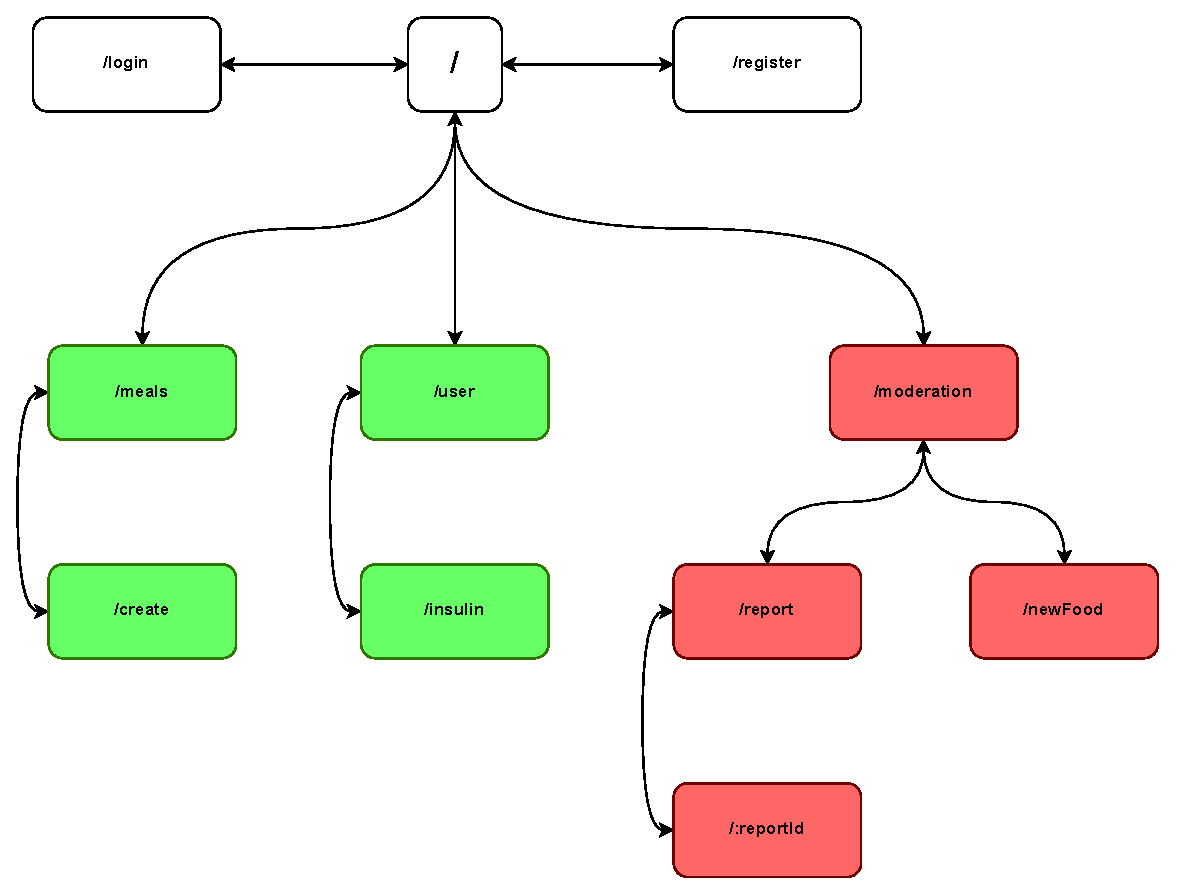
\includegraphics[scale=0.7]{_figures/web-client-endpoints.eps}
        \caption{The web client's navigation diagram}
    \end{center}
\end{figure}

\subsubsection{Error handling}

Whenever an HTTP request is sent to the server and an error occurs, the application takes
advantage of the \textbf{problem-json} content-type to display a specialized error message
to the user. When this is not possible, a generic error message is displayed instead.\\

\subsection{Functionalities}

\subsubsection{Register and login}

\begin{figure}[H]
    \begin{center}
        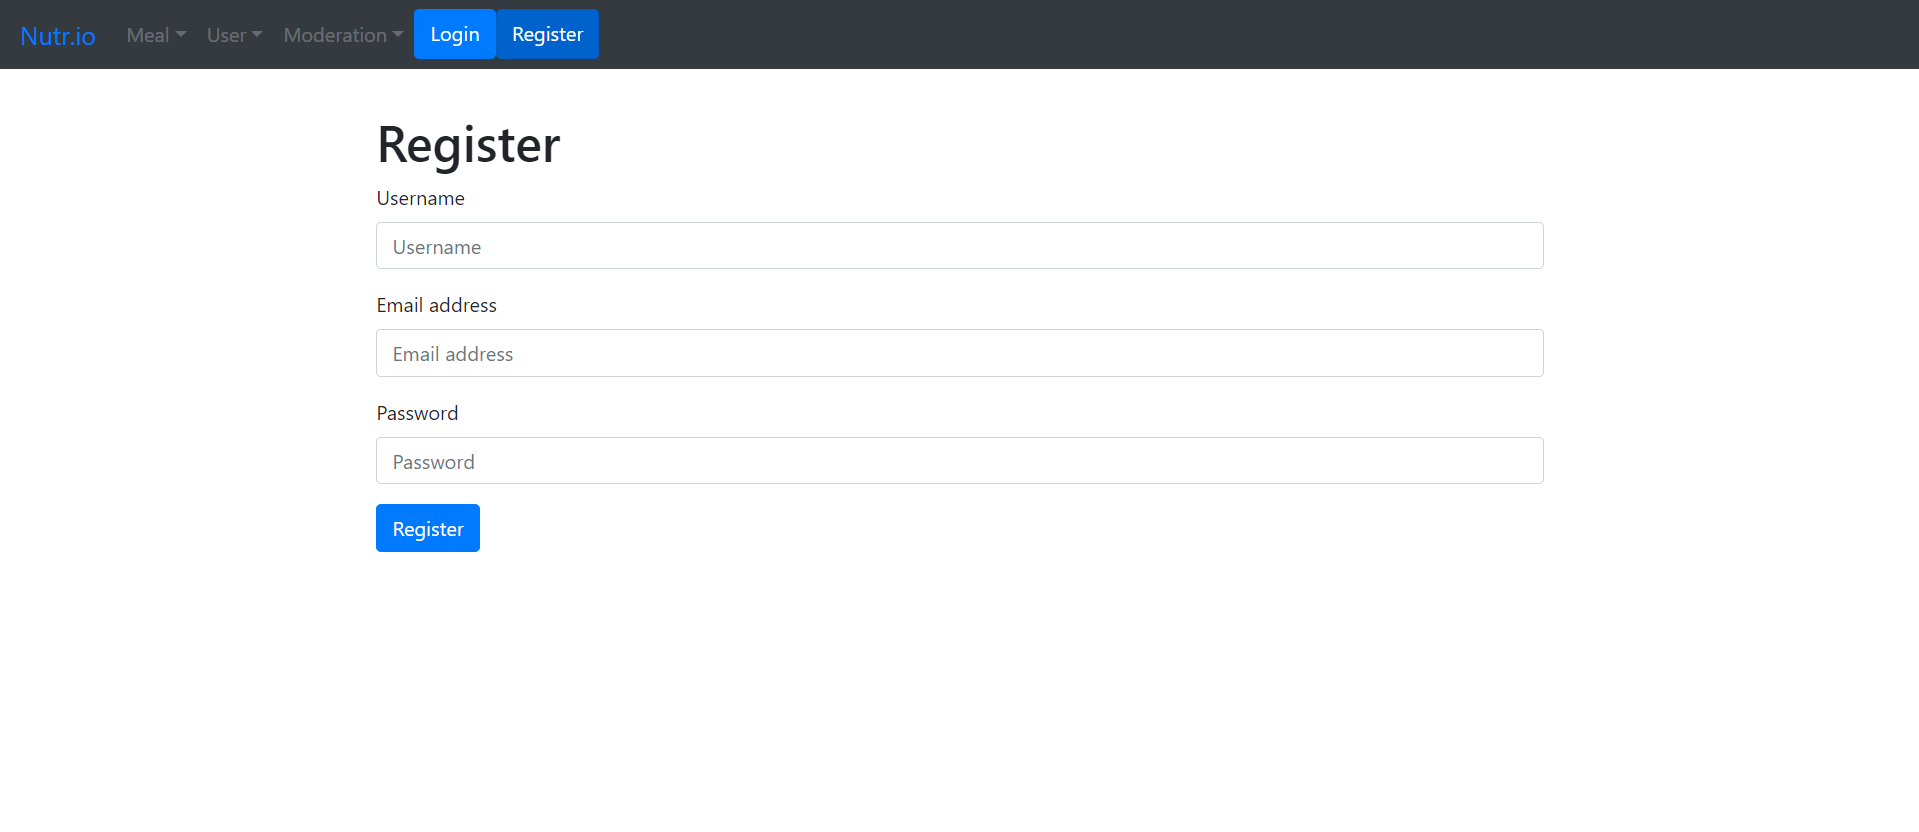
\includegraphics[scale=0.4]{_figures/register-page.png}
        \caption{Register and login page}
    \end{center}
\end{figure}

It should be noted that the landing page will activate more options once the user has logged in.\\

\subsubsection{Moderator: Create a meal or ingredient}

This feature provides moderators a way to insert hardcoded meals and ingredients into the database without
needing to manually insert them using SQL queries.\\

\begin{figure}[H]
    \begin{center}
        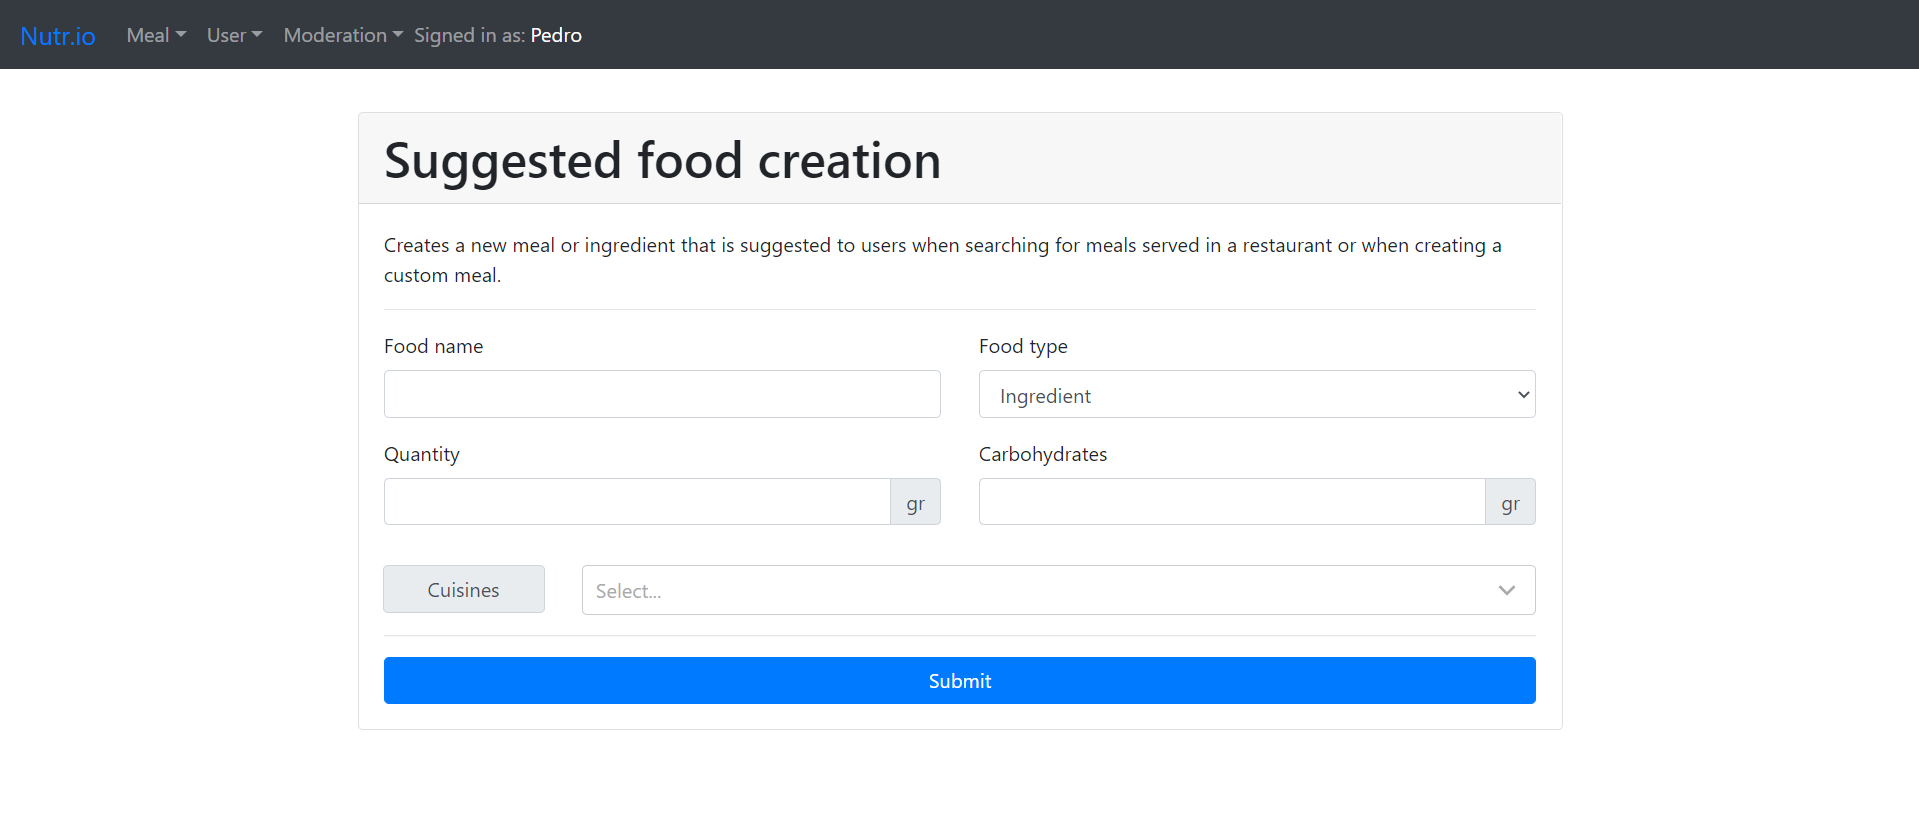
\includegraphics[scale=0.4]{_figures/hardcoded-meal-creation.png}
        \caption{Create a hardcoded meal or ingredient}
    \end{center}
\end{figure}

\subsubsection{User: Create a custom meal}

Meal creation is done in 5 steps and each can only be advanced when all fields are valid.
Going back and forth on each step remembers your choices, so editing a previous input is not cumbersome to the user.\\

The sum of all ingredient quantities can not be higher than the original quantity. 
But a meal can always have a leftover quantity which is considered undefined ingredient(s) or ingredients with no carbs.\\

\begin{figure}[H]
    \begin{center}
        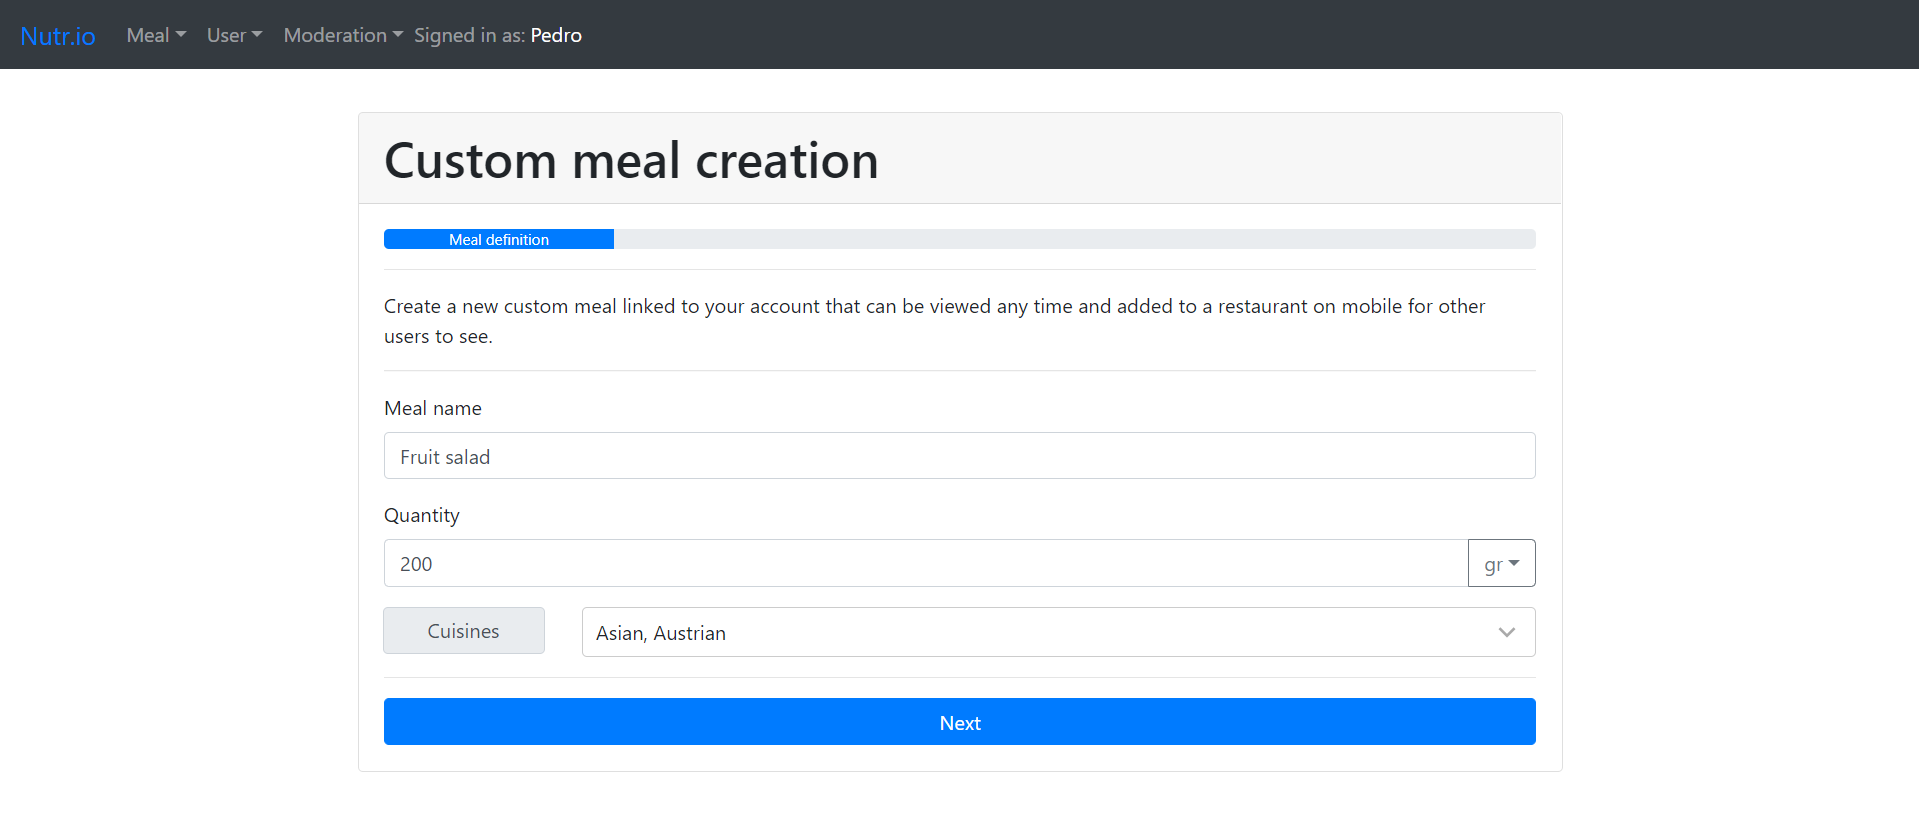
\includegraphics[scale=0.4]{_figures/custom-1.png}
        \caption{Meal description (name, quantity and cuisines)}
    \end{center}
\end{figure}

\begin{figure}[H]
    \begin{center}
        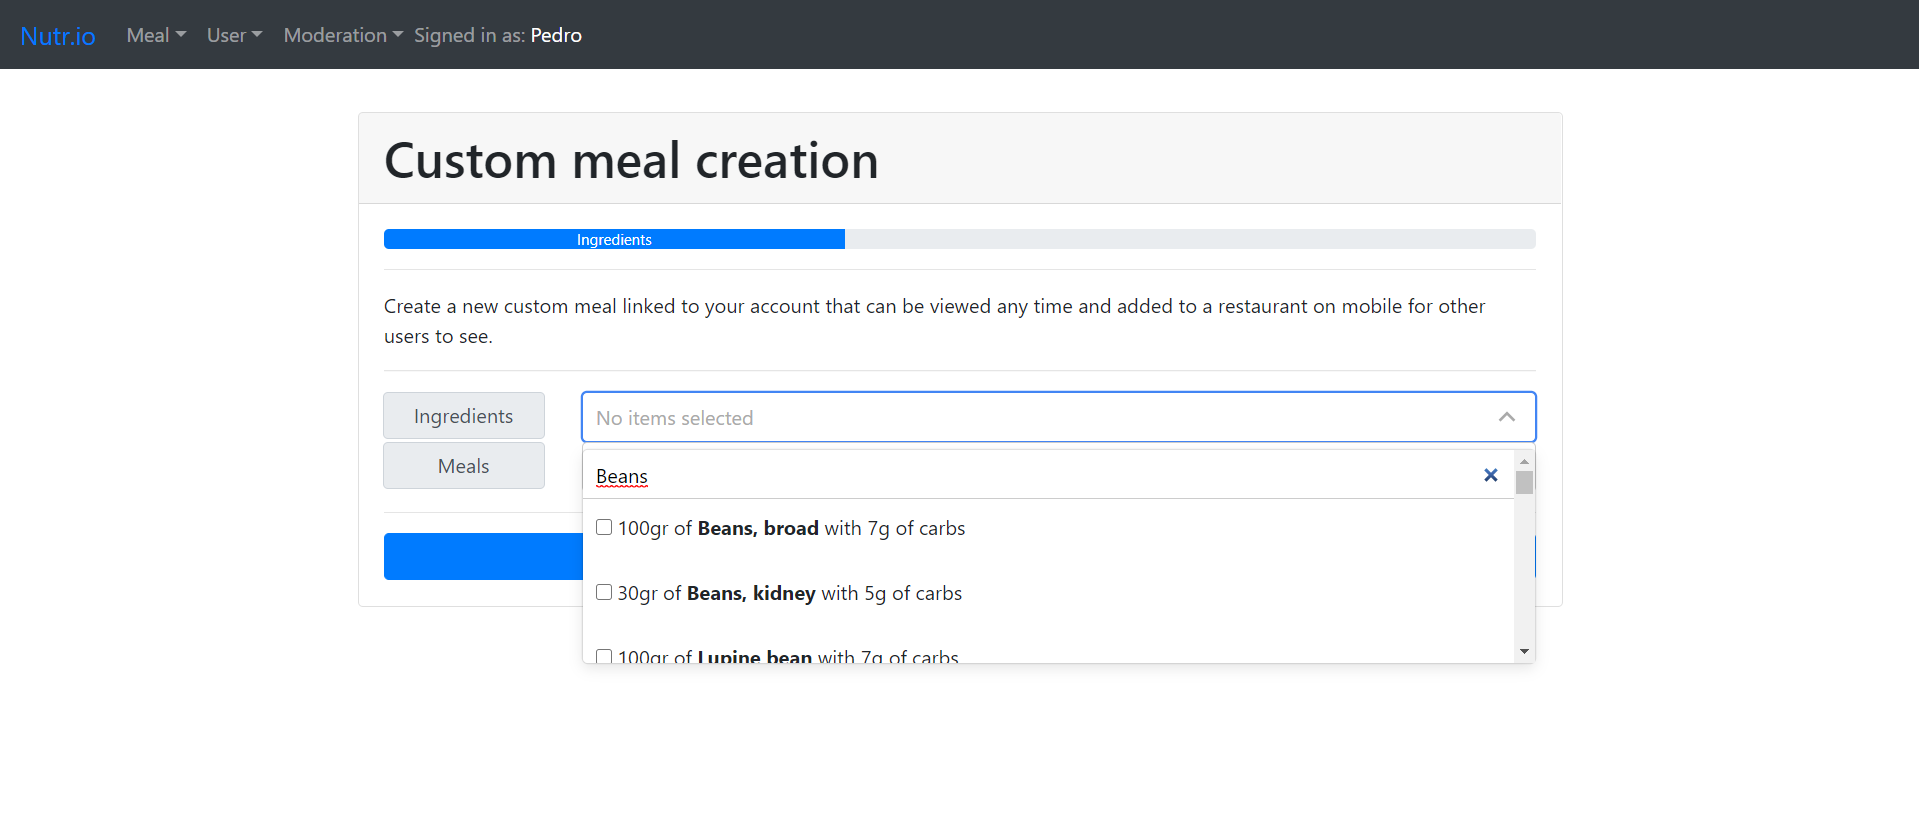
\includegraphics[scale=0.4]{_figures/custom-2.png}
        \caption{Ingredients (in the form of basic ingredients and other complex meals) are chosen}
    \end{center}
\end{figure}

\begin{figure}[H]
    \begin{center}
        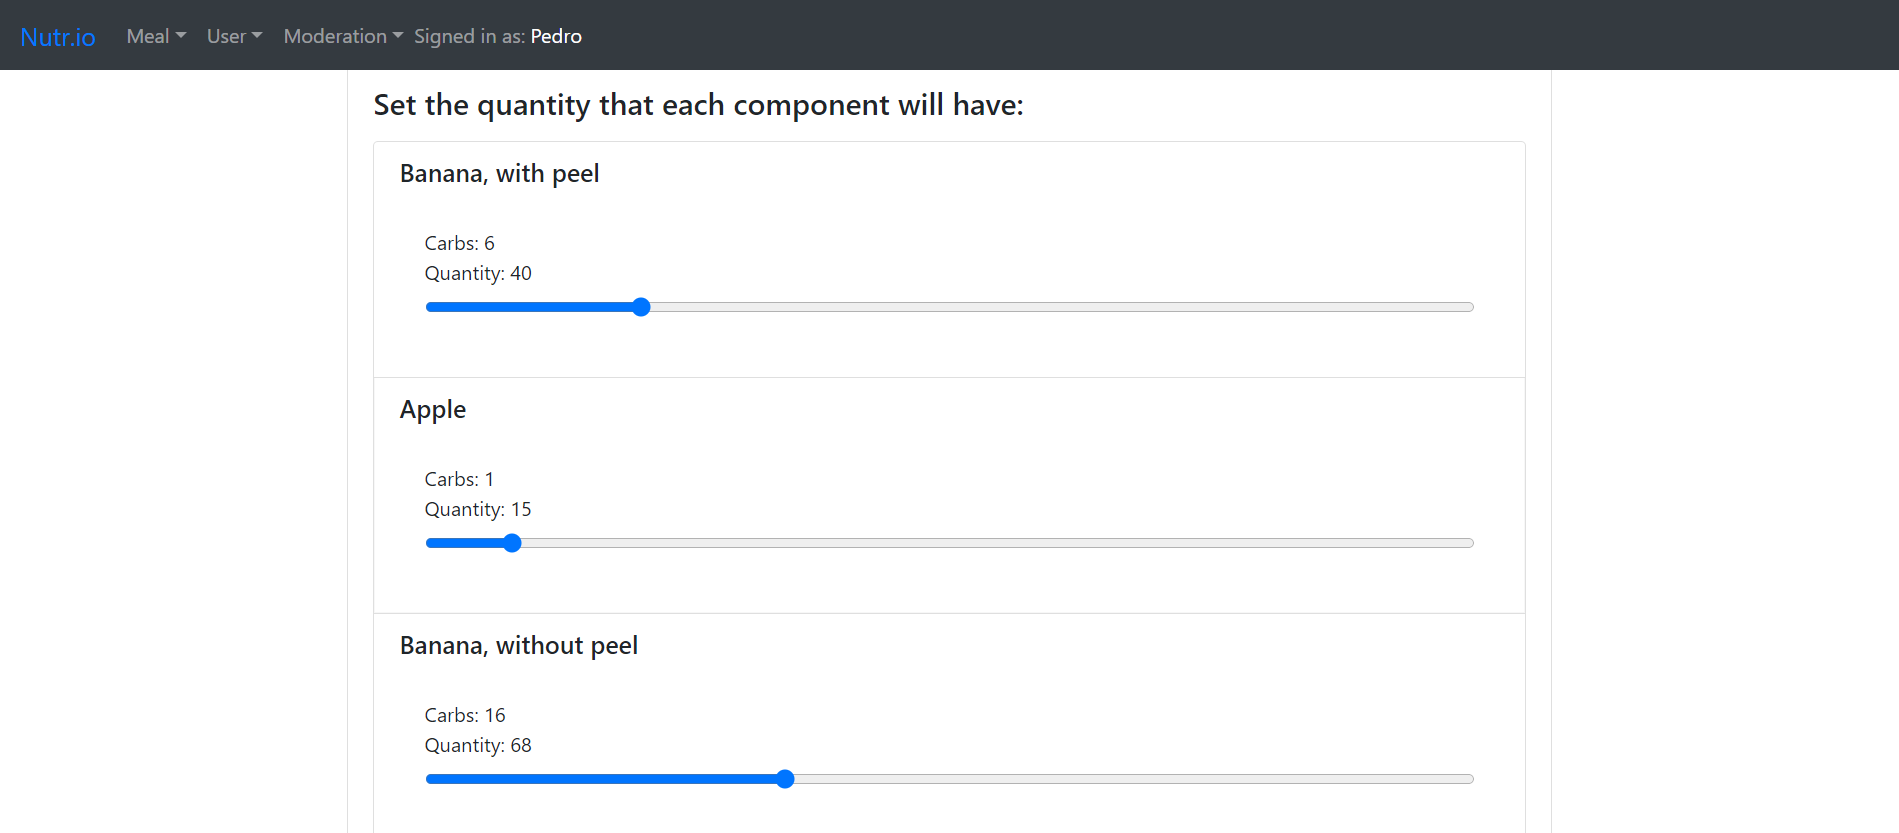
\includegraphics[scale=0.4]{_figures/custom-3.png}
        \caption{User chooses quantity for all chosen ingredients}
    \end{center}
\end{figure}

\begin{figure}[H]
    \begin{center}
        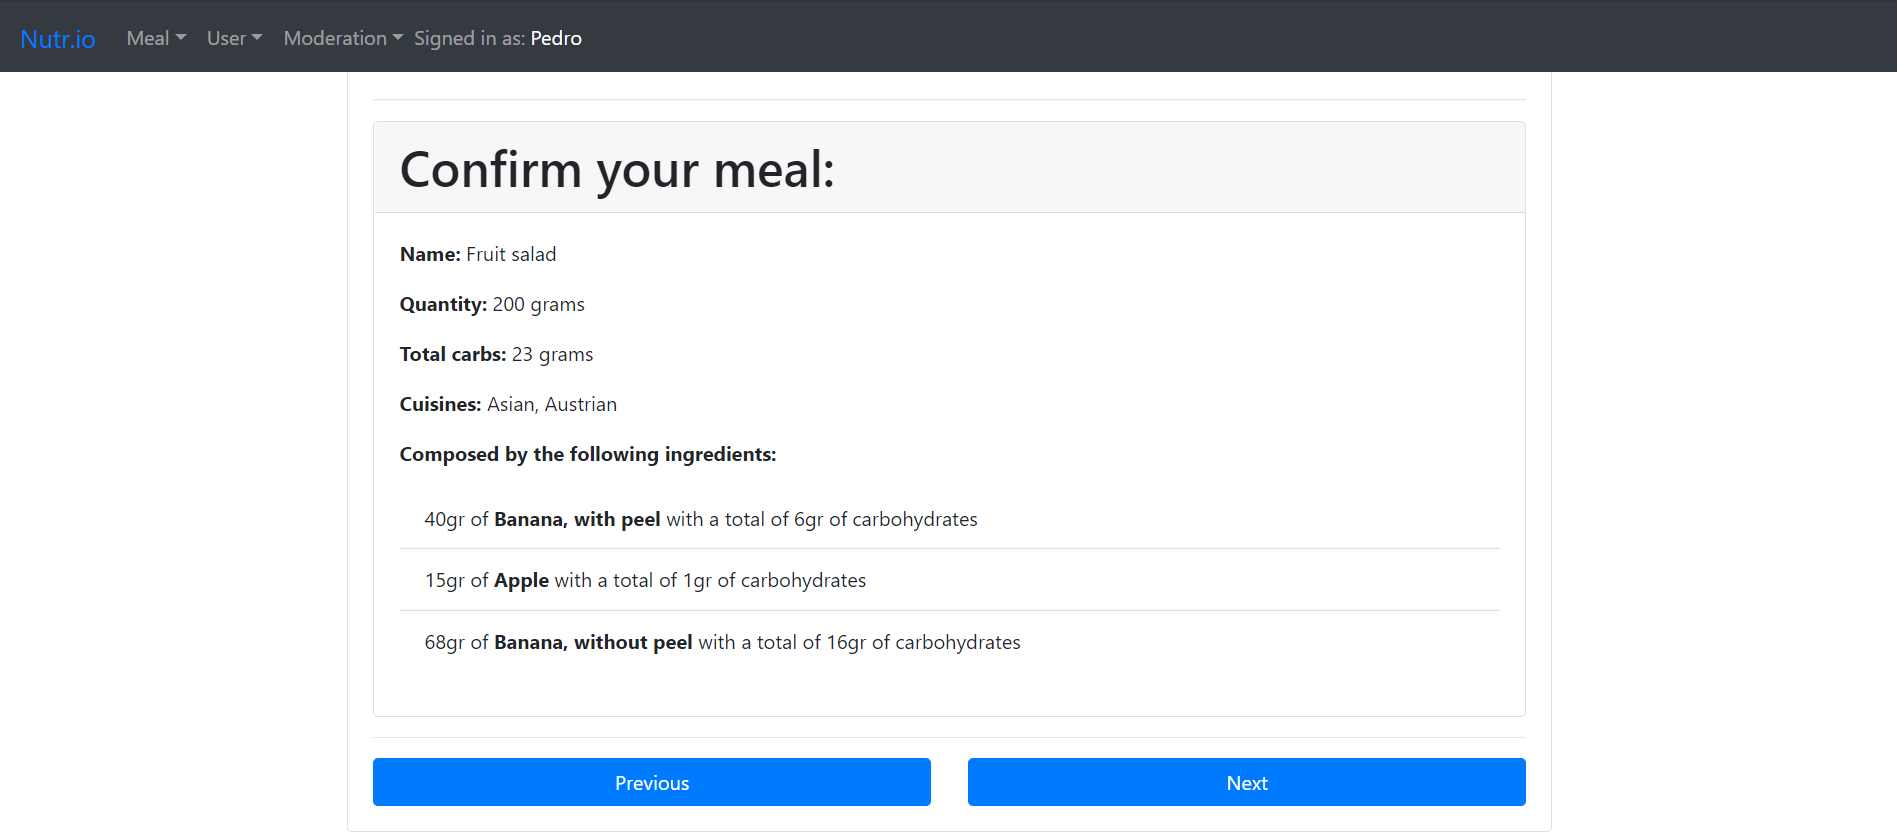
\includegraphics[scale=0.4]{_figures/custom-4.png}
        \caption{Input confirmation}
    \end{center}
\end{figure}

\begin{figure}[H]
    \begin{center}
        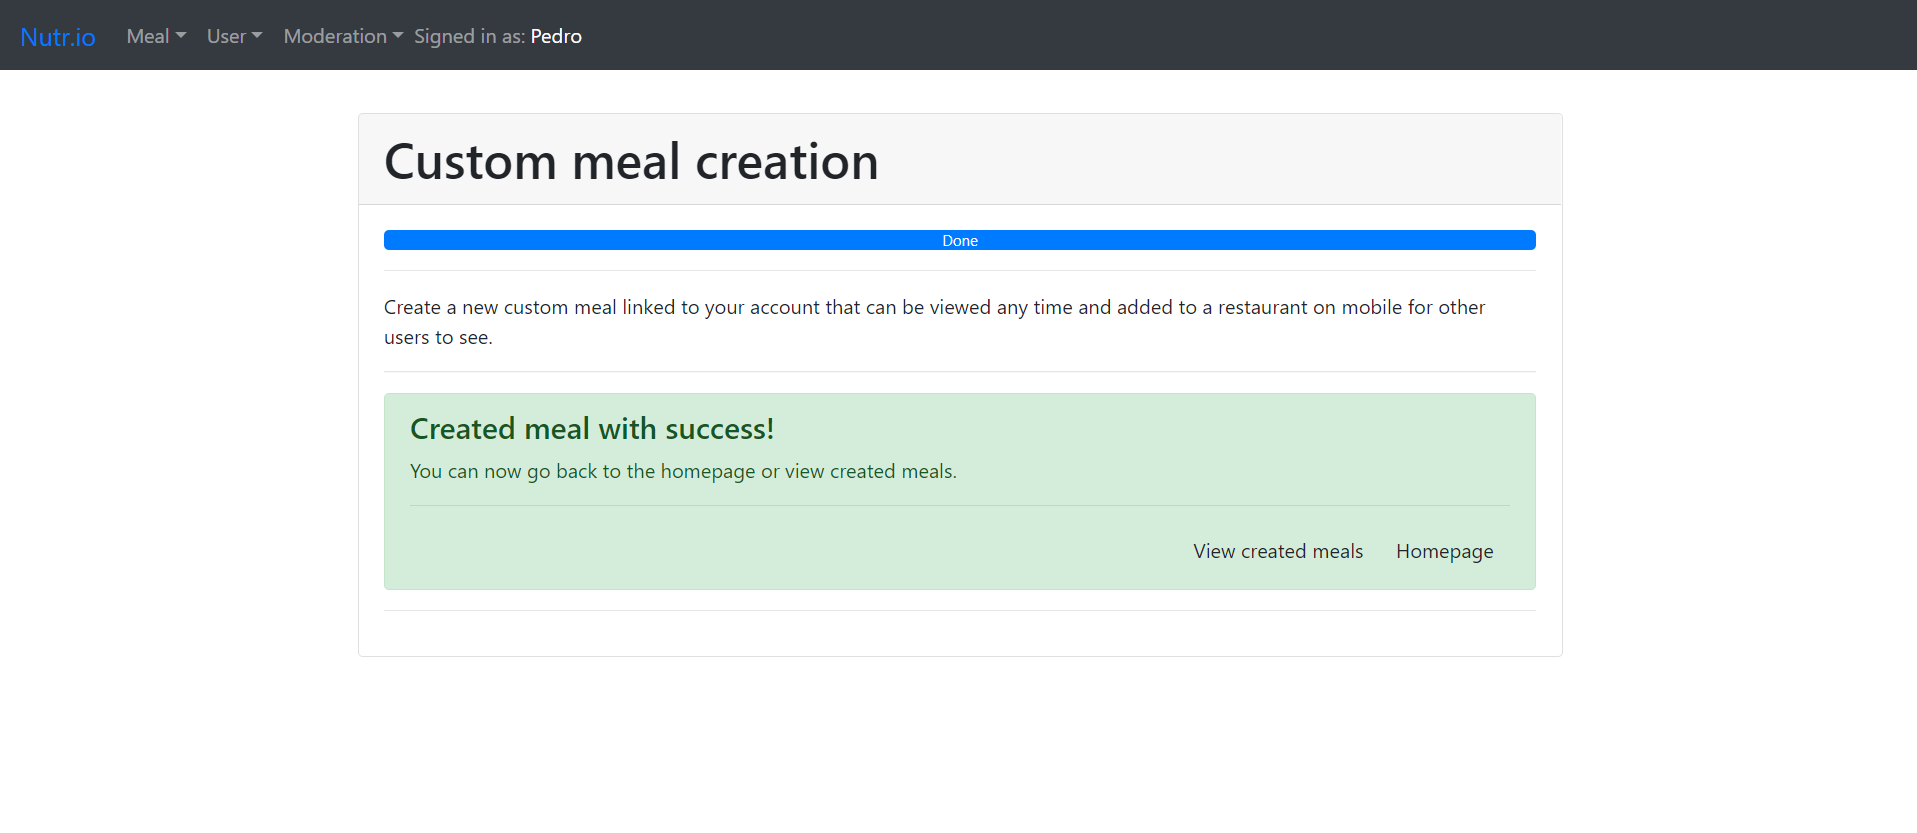
\includegraphics[scale=0.4]{_figures/custom-5.png}
        \caption{Send}
    \end{center}
\end{figure}

\subsubsection{User: Create an insulin profile}

Like in the mobile application, the user can also create insulin profiles by filling in this form 
and moving the slider to adjust their time periods.\\

If certain time periods are already taken by other created insulin profiles, these will appear with
gray tone inside the slider.\\

\begin{figure}[H]
    \begin{center}
        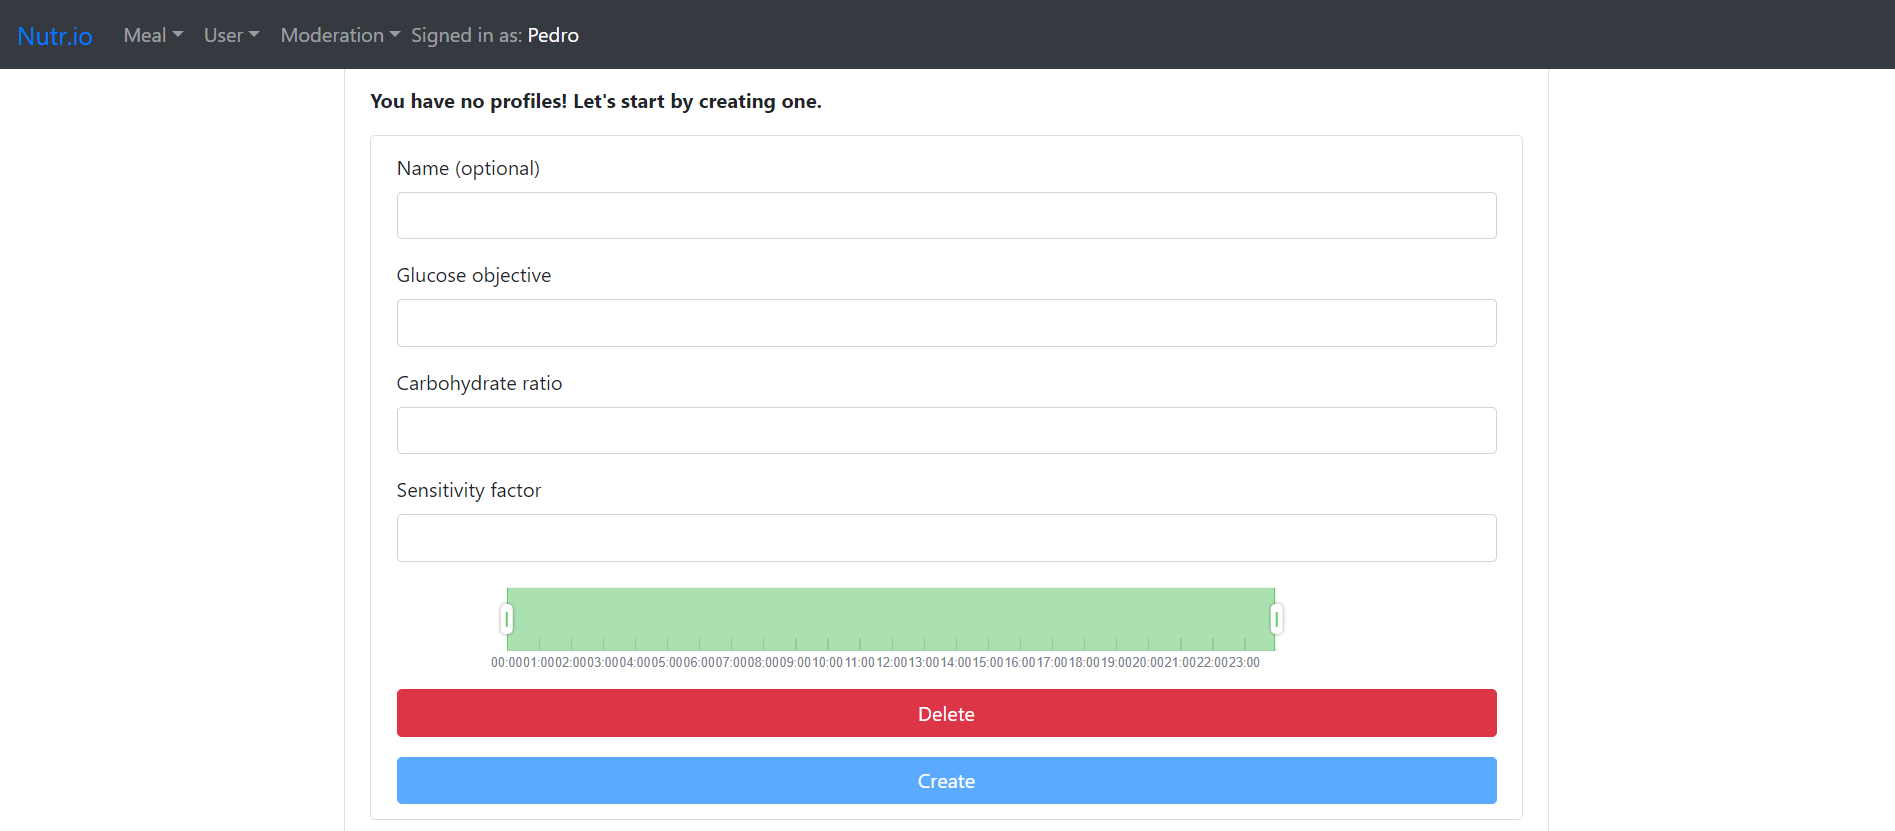
\includegraphics[scale=0.4]{_figures/web-insulin-profile-creation.png}
        \caption{Insulin profile creation}
    \end{center}
\end{figure}

\subsubsection{Moderator: Consult reports}

\begin{figure}[H]
    \begin{center}
        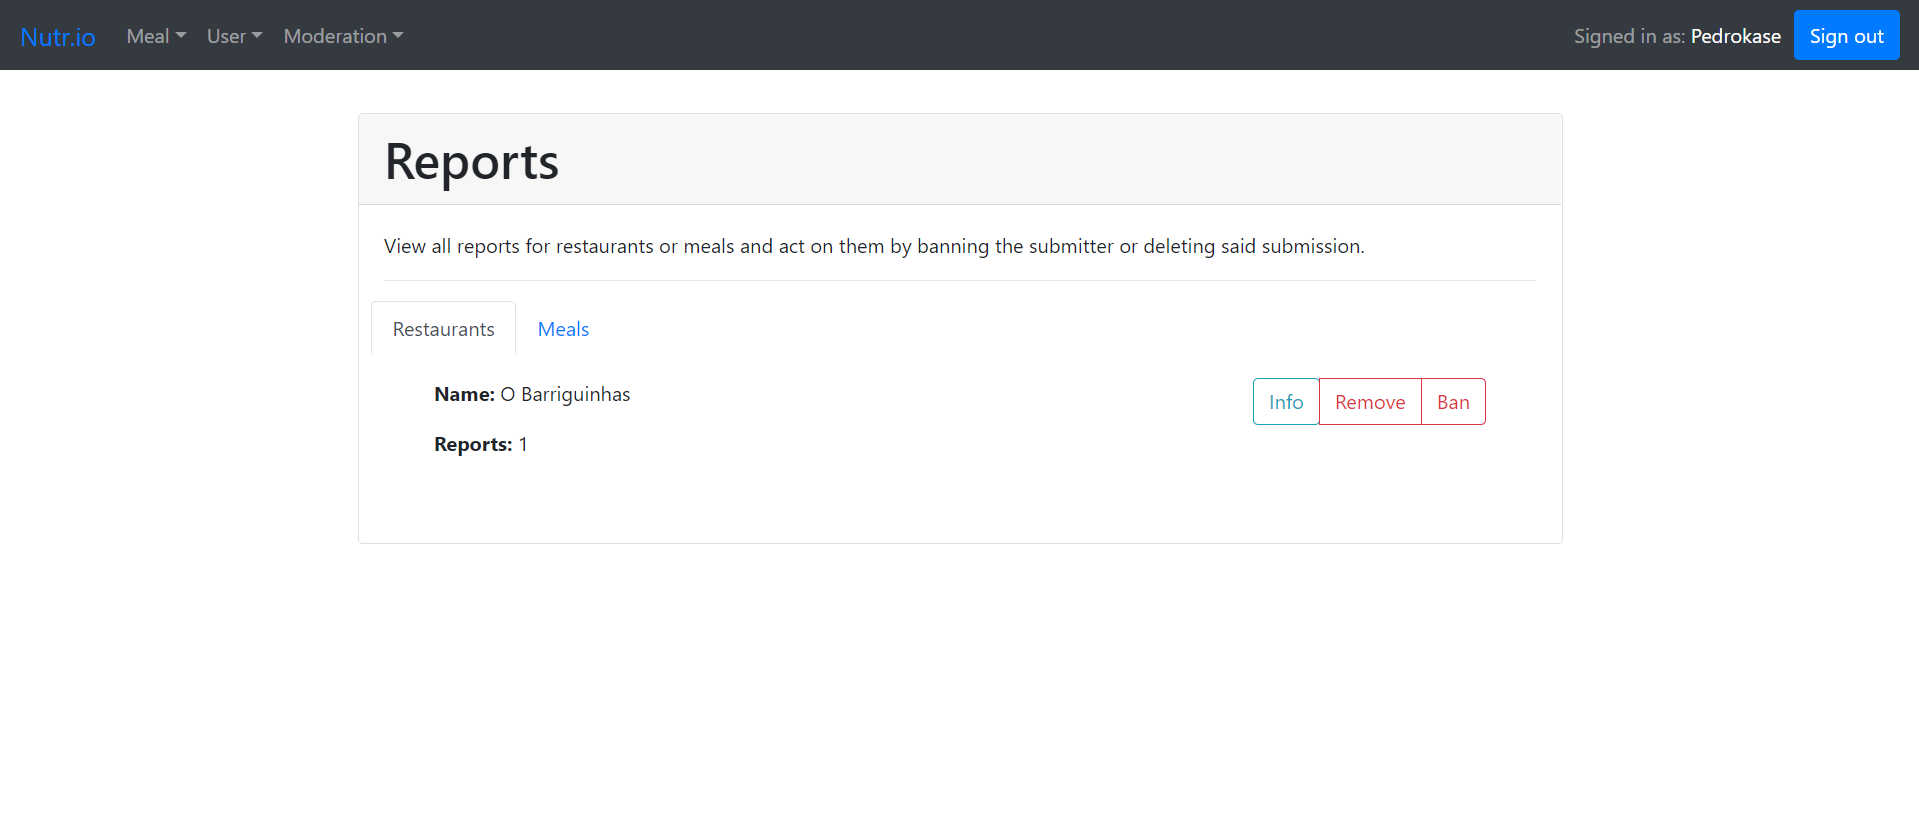
\includegraphics[scale=0.1, width=\textwidth]{_figures/reports.png}
        \caption{List of reports (restaurants and meals)} 
    \end{center}
\end{figure}

\begin{figure}[H]
    \begin{center}
        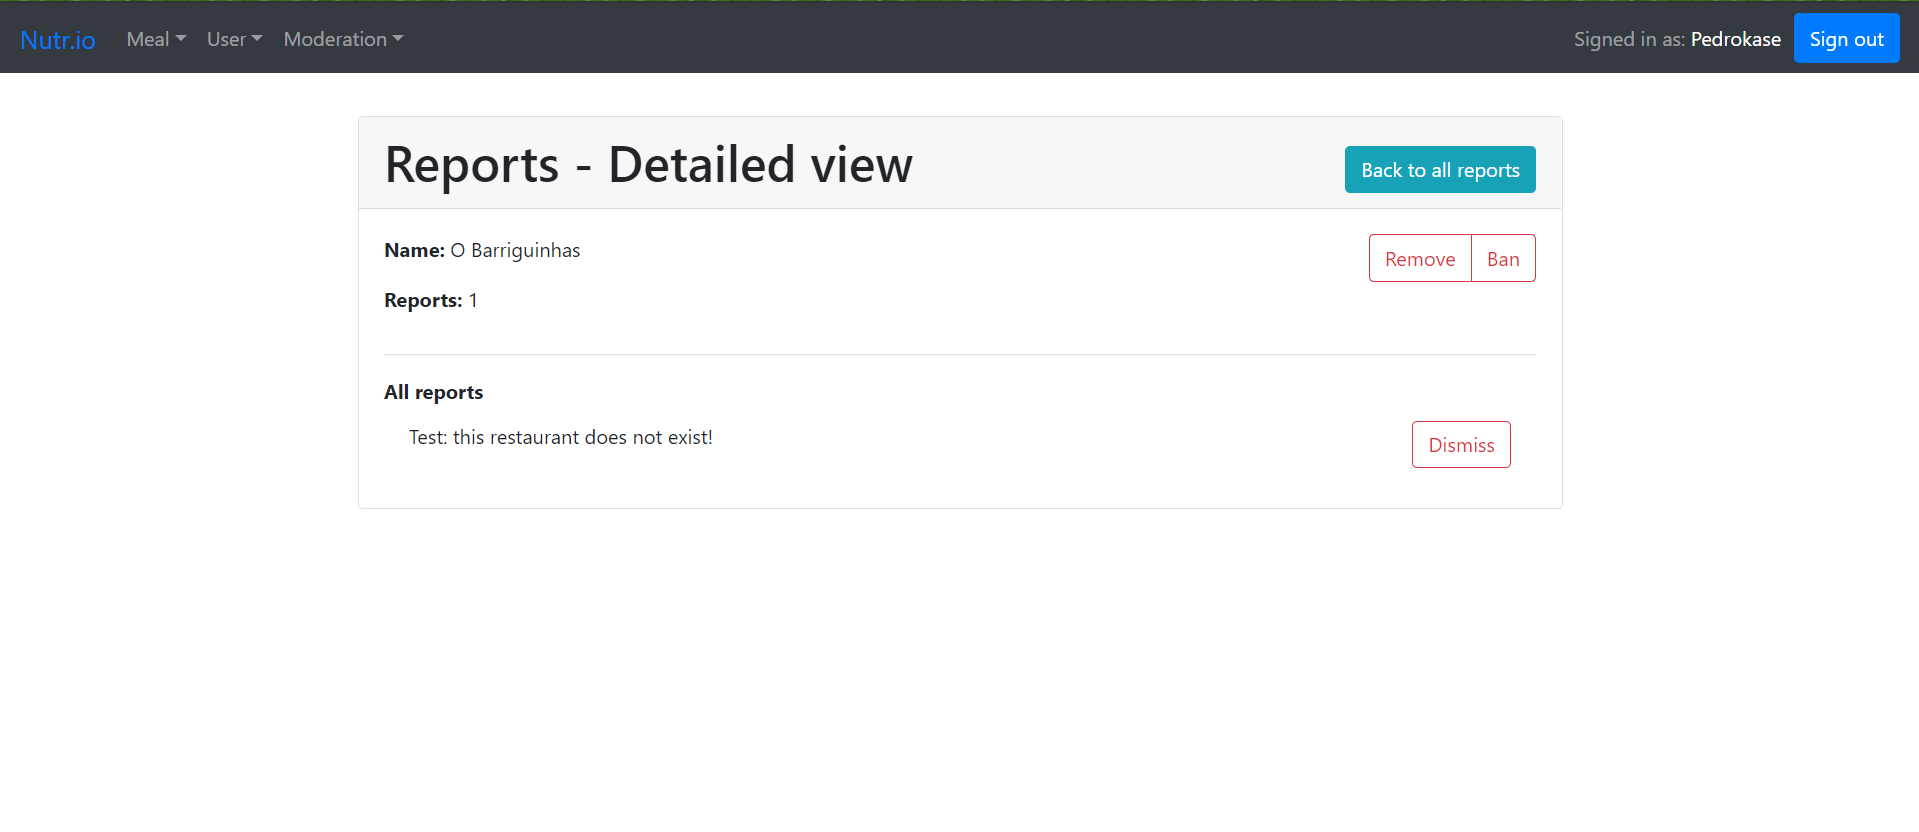
\includegraphics[scale=0.1, width=\textwidth]{_figures/detailed-report.png}
        \caption{A reports detail} 
    \end{center}
\end{figure}

Observing a report, a moderator has the options either to remove the faulty submission or ban
the user who submitted it.\\

\section{Deployment}

As planned, we decided to deploy the server to the Heroku\cite{heroku} cloud platform, to do this we had to follow a procedure and change some settings presented below.\\

After setting up the CLI tool and creating an app inside Heroku, we started to install the Heroku Postgres plugin which will provide our database to the
deployed server.

Configured the plugin, the next step was to create a file called \texttt{system.properties} inside
the server's root directory with the following setting: \texttt{java.runtime.version=11}. This setting forces Heroku to setup the
environment with Java JDK 11 when deploying the remote app.\\

The next step was to create the environment variables, which were being used during development inside the 
application settings.\\

As the Heroku application has now our database, the plugin automatically created a environment variable to link the server to the remote
tables and, as such, the \texttt{spring.datasource.url} value inside the \texttt{application.properties} needed to be changed to that 
variable name, as shown below.\\

\begin{figure}[H]
    \begin{center}
        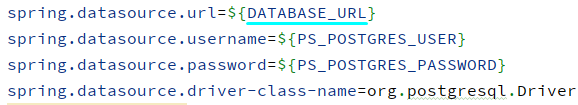
\includegraphics[scale=0.5]{_figures/heroku-env-db.png}
        \caption{Environment variable change inside application.properties} 
    \end{center}
\end{figure}

The last procedure to do before deployment is to run the command \texttt{npm run-script build}
inside the web client folder, which will execute a script that copies the web client's 
\texttt{index.html} and \texttt{main.js} to the HTTP server resources folder, in order to 
send HTML when an endpoint is being requested for the first time by a client. It is also important
to note that the web client is a single-page application, thus only the first request will send
HTML + JSON and the consequents only JSON, as the HTML will be cached inside the user's browser.\\

Concluded those steps, a successful deployment can now be achieved by following the commands inside
application's deploy tab.


